\documentclass[twoside,12pt,openany]{book}
\usepackage{fontspec} 
\usepackage[utf8]{inputenc} 
\newfontfamily{\arial}{Arial Unicode MS}
\newfontfamily\EmojiFont{Segoe UI Emoji}[Renderer=Harfbuzz]
\newcommand{\emoji}[1]{{\EmojiFont #1}}
% 默认字体保持LaTeX标准设置
% 中文支持设置
% 使用ctex包但不使用默认字体设置(fontset=none)
\usepackage[fontset=none]{ctex}
% 设置中文字体:宋体为主字体,黑体为粗体,楷体为斜体
\setCJKmainfont{SimSun}[
  BoldFont = SimHei,
  ItalicFont = KaiTi,
  BoldItalicFont = KaiTi
]


\renewcommand{\floatpagefraction}{.9}
\renewcommand{\topfraction}{.9}
\renewcommand{\bottomfraction}{.9}
\renewcommand{\textfraction}{.1}
\setcounter{totalnumber}{50}
\setcounter{topnumber}{50}
\setcounter{bottomnumber}{50}


% 加载常用包
\usepackage{tcolorbox}  % 彩色文本框支持
\usepackage{ulem}
\usepackage{silence}
\WarningFilter{latex}{Overfull \hbox}
\usepackage[absolute, overlay]{textpos}
\setlength{\TPHorizModule}{1mm}
\setlength{\TPVertModule}{1mm}
\tcbuselibrary{skins, breakable}  % 加载tcolorbox的皮肤和断页功能
\usepackage{tikz}  % 绘图支持
\usepackage{afterpage}
\usepackage{graphicx}  % 图片插入支持
\graphicspath{{figures/},{figures/部门1/},{figures/部门2/},{figures/看板/},{figures/头像/},{figures/部酱/},{figures/页眉页脚/},{figures/章节首页/},{figures/活动/}}  % 设置图片路径为figures目录
% 颜色和页面布局设置
\usepackage{xcolor}  % 颜色支持
\usepackage{wrapfig}  % 文字环绕图片支持
\usepackage{floatflt}
\usepackage{eso-pic}  % 页面背景支持
\usepackage{geometry}  % 页面布局设置
\usepackage{setspace}
\usepackage{textcomp}
%\usepackage{showframe}
\usepackage{pifont}
\usepackage{fancyhdr}
\usepackage{comment}
\usepackage{adjustbox}
\usepackage{eso-pic}
\usepackage{ragged2e}
\usepackage{tikz}
\usetikzlibrary{shapes.geometric}
\usepackage{multicol}
\usepackage{enumitem}
\newenvironment{categorysection}[1]{
  \subsection*{\textcolor{truepurple}{#1}}
  \begin{itemize}[leftmargin=*, 
                 nosep,               % 移除所有额外间距
                 itemsep=2pt,         % 条目间距=0
                 parsep=0pt,          % 段落间距=0
                 before=\setlength{\baselineskip}{23pt} % 设置行距
  ]
}{
  \end{itemize}
}
\usetikzlibrary{calc,positioning}
\usetikzlibrary{shapes, arrows}  

\geometry{a4paper, left=1.5cm, right=1.5cm, top=2cm, bottom=2.5cm}
% 设置无衬线中文字体为黑体
\setCJKsansfont{SimHei}

% 定义文档使用的颜色
\definecolor{truepurple}{RGB}{128, 0, 128}  % 主色调紫色
\definecolor{taopink}{HTML}{F17F98}  % 桃子名字
\definecolor{tao}{HTML}{FFF2F9}  % 桃子气泡
\definecolor{zi}{HTML}{F8F2F9}  % 紫荆气泡
\definecolor{qing}{HTML}{F2F9EA}  % 清芬气泡
\definecolor{default}{HTML}{F9F9F9}  %默认气泡灰
% 加载tikz的渐变效果库
\usetikzlibrary{fadings}

% 页面布局设置
\geometry{
  top=1.5cm,       % 从3cm减小到1.5cm
  headheight=20.57637pt, % 解决fancyhdr警告
  headsep=10pt,     % 增加页眉与正文间距
  footskip=30pt     % 增加页脚与正文间距
}

% 定义聊天气泡样式
% 使用说明:
% \chatbubble[位置]{头像路径}{昵称}{消息内容}{背景颜色}
% 可选参数:
% [left] - 左侧气泡(默认)
% [right] - 右侧气泡
% 示例:
% \chatbubble[left]{taozi.jpg}{桃子}{消息内容}{tao}
% \chatbubble[right]{zijing.jpg}{紫荆}{消息内容}{zi}
% \chatbubble[right]{qingfen.jpg}{清芬}{消息内容}{qing}
\newcounter{chatcounter}
\newcommand{\chind}{\hspace*{2em}}
\newcommand{\chatbubble}[5][left]{%
  \stepcounter{chatcounter}%
  \par\noindent%
  \ifstrequal{#1}{left}
    {% 左侧气泡
     \begin{minipage}[t]{1.2cm} % 头像宽度
        \begin{tikzpicture}[baseline=(current bounding box.center)]
          \node[circle, draw=gray!50, line width=0.5pt, minimum size=1.2cm, 
                path picture={\node at (path picture bounding box.center) 
                {\includegraphics[width=1.2cm]{#2}};}] {};
        \end{tikzpicture}
     \end{minipage}%
     \hspace{0.2cm}%
     \begin{minipage}[t]{0.7\textwidth} % 消息框宽度
        \vspace{-15pt} % 确保顶部对齐
        \noindent\textcolor{darkgray!80}{\sffamily #3} % 昵称
        \vspace{5pt}
        \begin{tcolorbox}[
          enhanced,
          breakable=false,
          colback={#5},
          colframe={#5},
          arc=8pt,
          boxrule=0.5pt,
          left=8pt,
          right=8pt,
          top=4pt,
          bottom=4pt,
          before skip=0pt,
          after skip=10pt,
          width=\linewidth,
          before upper={\setlength{\parindent}{0em} \setlength{\parskip}{0pt}},
        ]
          #4
        \end{tcolorbox}
     \end{minipage}
    }
    {% 右侧气泡
     \hfill%
     \begin{minipage}[t]{0.7\textwidth} % 消息框宽度
        \vspace{-15pt} % 确保顶部对齐
        \noindent\hfill\textcolor{darkgray!80}{\sffamily #3} % 右对齐昵称
        \vspace{5pt}
        \hfill%
        \begin{tcolorbox}[
          enhanced,
          breakable=false,
          colback={#5},
          colframe={#5},
          arc=8pt,
          boxrule=0.5pt,
          left=8pt,
          right=8pt,
          top=4pt,
          bottom=4pt,
          before skip=0pt,
          after skip=10pt,
          width=\linewidth,
          before upper={\setlength{\parindent}{0em} \setlength{\parskip}{0pt}},
        ]
          #4
        \end{tcolorbox}
     \end{minipage}%
     \hspace{0.2cm}%
     \begin{minipage}[t]{1.2cm} % 头像宽度
        \begin{tikzpicture}[baseline=(current bounding box.center)]
          \node[circle, draw=gray!50, line width=0.5pt, minimum size=1.2cm, 
                path picture={\node at (path picture bounding box.center) 
                {\includegraphics[width=1.2cm]{#2}};}] {};
        \end{tikzpicture}
     \end{minipage}
    }%
  \par\vspace{0.1cm}% 气泡间距
}
\newcommand{\picbox}[1]{%
\vspace{0.3em}

    \begin{tikzpicture}
        \node[
            trapezium, 
            draw=truepurple, 
            fill=truepurple!80!black, 
            text=white, 
            inner sep=3pt, 
            minimum width=0.8\linewidth, % 宽度为行宽的80%
            minimum height=0.3cm, 
            trapezium left angle=90, % 左边直角
            trapezium right angle=65, % 右边角度
            trapezium stretches=true, % 允许拉伸
            align=left % 文本居左
        ] 
        {#1};
    \end{tikzpicture}%
}
% 设置页眉页脚样式
\pagestyle{fancy}  % 使用fancy页眉页脚样式
\fancyhf{} % 清空所有页眉页脚默认设置

% 设置页眉
% LE: 偶数页左侧页眉
\fancyhead[LE]{\hspace*{-1.5cm}\includegraphics[width=\paperwidth]{head.pdf}} 
% RO: 奇数页右侧页眉
\fancyhead[RO]{\hspace*{-1.5cm}\includegraphics[width=\paperwidth]{headr.pdf}} 
\renewcommand{\headrulewidth}{0pt}  % 移除页眉分隔线
\setlength{\headsep}{5mm}  % 设置页眉与正文间距

% 设置页脚
% LE: 偶数页左侧页脚
\fancyfoot[LE]{\hspace{-0.3cm}\raisebox{-13pt}{\textcolor{white}{\textbf{\textsf{\thepage}}}}} 
% RO: 奇数页右侧页脚
\fancyfoot[RO]{\rlap{\hspace{-0.15cm}\raisebox{-13pt}{\textcolor{white}{\textbf{\textsf{\thepage}}}}}}
\renewcommand{\footrulewidth}{0pt}  % 移除页脚分隔线

% 添加页面背景图片
% 根据奇偶页显示不同的背景图片
\AddToShipoutPictureBG{%
  \ifodd\value{page}
    % 奇数页底部背景
    \AtPageLowerLeft{%
      \raisebox{15pt}[0pt][0pt]{\includegraphics[width=\paperwidth]{footr.pdf}}%
    }
  \else
    % 偶数页底部背景
    \AtPageLowerLeft{%
      \raisebox{15pt}[0pt][0pt]{\includegraphics[width=\paperwidth]{footl.pdf}}%
    }
  \fi
}
% 定义橙色
\definecolor{thuorange}{RGB}{247, 148, 29}

\begin{document}
% 目录页设置
\vspace*{0.7cm}  % 顶部间距
\begin{center}
    % 主标题
    \fontsize{30pt}{32pt}\selectfont
    \textbf{\textcolor{truepurple}{目录}}
    \\[0ex]  % 标题间距
    % 副标题
    \fontsize{18pt}{20pt}\selectfont
    \textcolor{thuorange}{Contents}
\end{center}
% 目录内容
\begin{Large}
\doublespacing  % 双倍行距
社团介绍\\ 
主要活动介绍\\
社团Q\&A\\
分部介绍
\begin{large}
\begin{itemize}
  \item 组织部门
  \item 创作类
  \item 歌舞艺术类
  \item 综合类
  \item 作品类
  \item 游戏类
  \item 娱乐影视类
  \item 科技生活类
\end{itemize}
\end{large}
\vspace*{0.3cm}  % 项目间距
社员寄语
\end{Large}
\newpage  % 新的一页

% 第一章:社团介绍
% {{{ 第一页
\vspace*{0.7cm}  % 顶部间距

% 社团标题和logo布局
\begin{flushleft}
    % 主标题:中文社团名称
    \fontsize{30pt}{32pt}\selectfont
    \textbf{\textcolor{truepurple}{清华大学学生次世代动漫社}}
    \\[0ex]  % 标题间距
    % 副标题:英文社团名称
    \fontsize{18pt}{20pt}\selectfont
    \textcolor{thuorange}{THU Student New Era ACG Club}
    % 右侧图片:社团logo
    \vspace{-1cm} % 标题与图片的间距调整
    \noindent\hspace*{\dimexpr\textwidth-5cm-1cm}% 计算右侧对齐位置
    
\includegraphics[width=6.5cm]{thujisedai.jpg}  % 社团logo图片
\end{flushleft}
% 内容部分:两栏布局
\begin{flushleft}
    \begin{minipage}[t]{0.45\textwidth}  % 左侧栏
        \section*{\normalsize\textbf{\textcolor{truepurple}{社团理念}}}
        \vspace{-1em}
        \subsection*{\normalsize\textbf{\textcolor{thuorange}{Core Concepts}}}
        \vspace{-0em}
        \small
        \begin{itemize}
            \item \textbf{服务同好人群} \textit{Serve like-minded people}
            \item \textbf{支持原创力量} \textit{Support creative power}
            \item \textbf{宣传动漫文化} \textit{Promote ACG culture}
        \end{itemize}
        \vspace{0.7em}

        \section*{\normalsize\textbf{\textcolor{truepurple}{成立时间}}}
        \vspace{-1em}
        \subsection*{\normalsize\textbf{\textcolor{thuorange}{Time of Establishment}}}
        \vspace{-0.5em}
        
        \textbf{1999年}


        
    \end{minipage}
    \hfill  % 填充两栏之间的空间
    \begin{minipage}[t]{0.5\textwidth}  % 右侧栏
        \section*{\normalsize\textbf{\textcolor{truepurple}{职能部门}}}
        \vspace{-1em}
        \subsection*{\normalsize\textbf{\textcolor{thuorange}{Functional Department}}}
        \vspace{-0em}
        \small
        \textbf{组织部} \textit{Department of organization}
        \vspace{0.4em}
        \section*{\normalsize\textbf{\textcolor{truepurple}{兴趣部门}}}
        \vspace{-1em}
        \subsection*{\normalsize\textbf{\textcolor{thuorange}{Interest Departments}}}
        \vspace{-0.5em}
        \small
        \textbf{两百余个},包括泛ACGN领域各类兴趣爱好\\也欢迎组建新的部门!\\ \textit{More than 200, covering various fields of ACGN themes}. \\(And you can establish new departments if you want!)
    \end{minipage}
\end{flushleft}

\vfill  % 填充垂直空间

\vspace{0.5cm}  % 间距调整
% 社团荣誉部分
\begin{center}
    \Large\textbf{\textcolor{truepurple}{社团荣誉}}  % 中文标题
    \\[0ex]  % 标题间距
    \large\textbf{\textit{\textcolor{thuorange}{Club Honors}}}  % 英文标题
\end{center}

\vspace{0.5cm}  % 间距调整
\begin{flushleft}
    \begin{itemize}  % 荣誉列表
        \item[] \normalsize\textbf{2017-2018学年} \qquad 清华大学\textbf{十佳学生社团}
        \item[] \normalsize\textbf{2018-2019学年} \qquad 清华大学\textbf{十佳学生社团}
        \item[] \normalsize\textbf{2019-2020学年} \qquad 清华大学\textbf{十佳学生社团} “ 星空杯 ”
        \item[] \normalsize\textbf{2020-2021学年} \qquad 清华大学学生社团\textbf{优秀风采奖}
        \item[] \normalsize\textbf{2021-2022学年} \qquad 清华大学学生社团\textbf{优秀风采奖}
        \item[] \normalsize\textbf{2022-2023学年} \qquad 清华大学\textbf{最佳兴趣类学生社团}
        \item[] \normalsize\textbf{2023-2024学年} \qquad 清华大学\textbf{最佳兴趣类学生社团}
        \item[] \normalsize\textbf{2024-2025学年} \qquad 清华大学\textbf{最佳兴趣类学生社团}
    \end{itemize}
\end{flushleft}

\vfill
% 部门列表部分
\newpage  % 新的一页
\normalsize
    \thispagestyle{empty} % 移除本页的页眉和页脚[8,9](@ref)
    \newgeometry{margin=0pt} % 临时将本页的页边距全部设置为0[1](@ref)
    \noindent % 防止缩进
    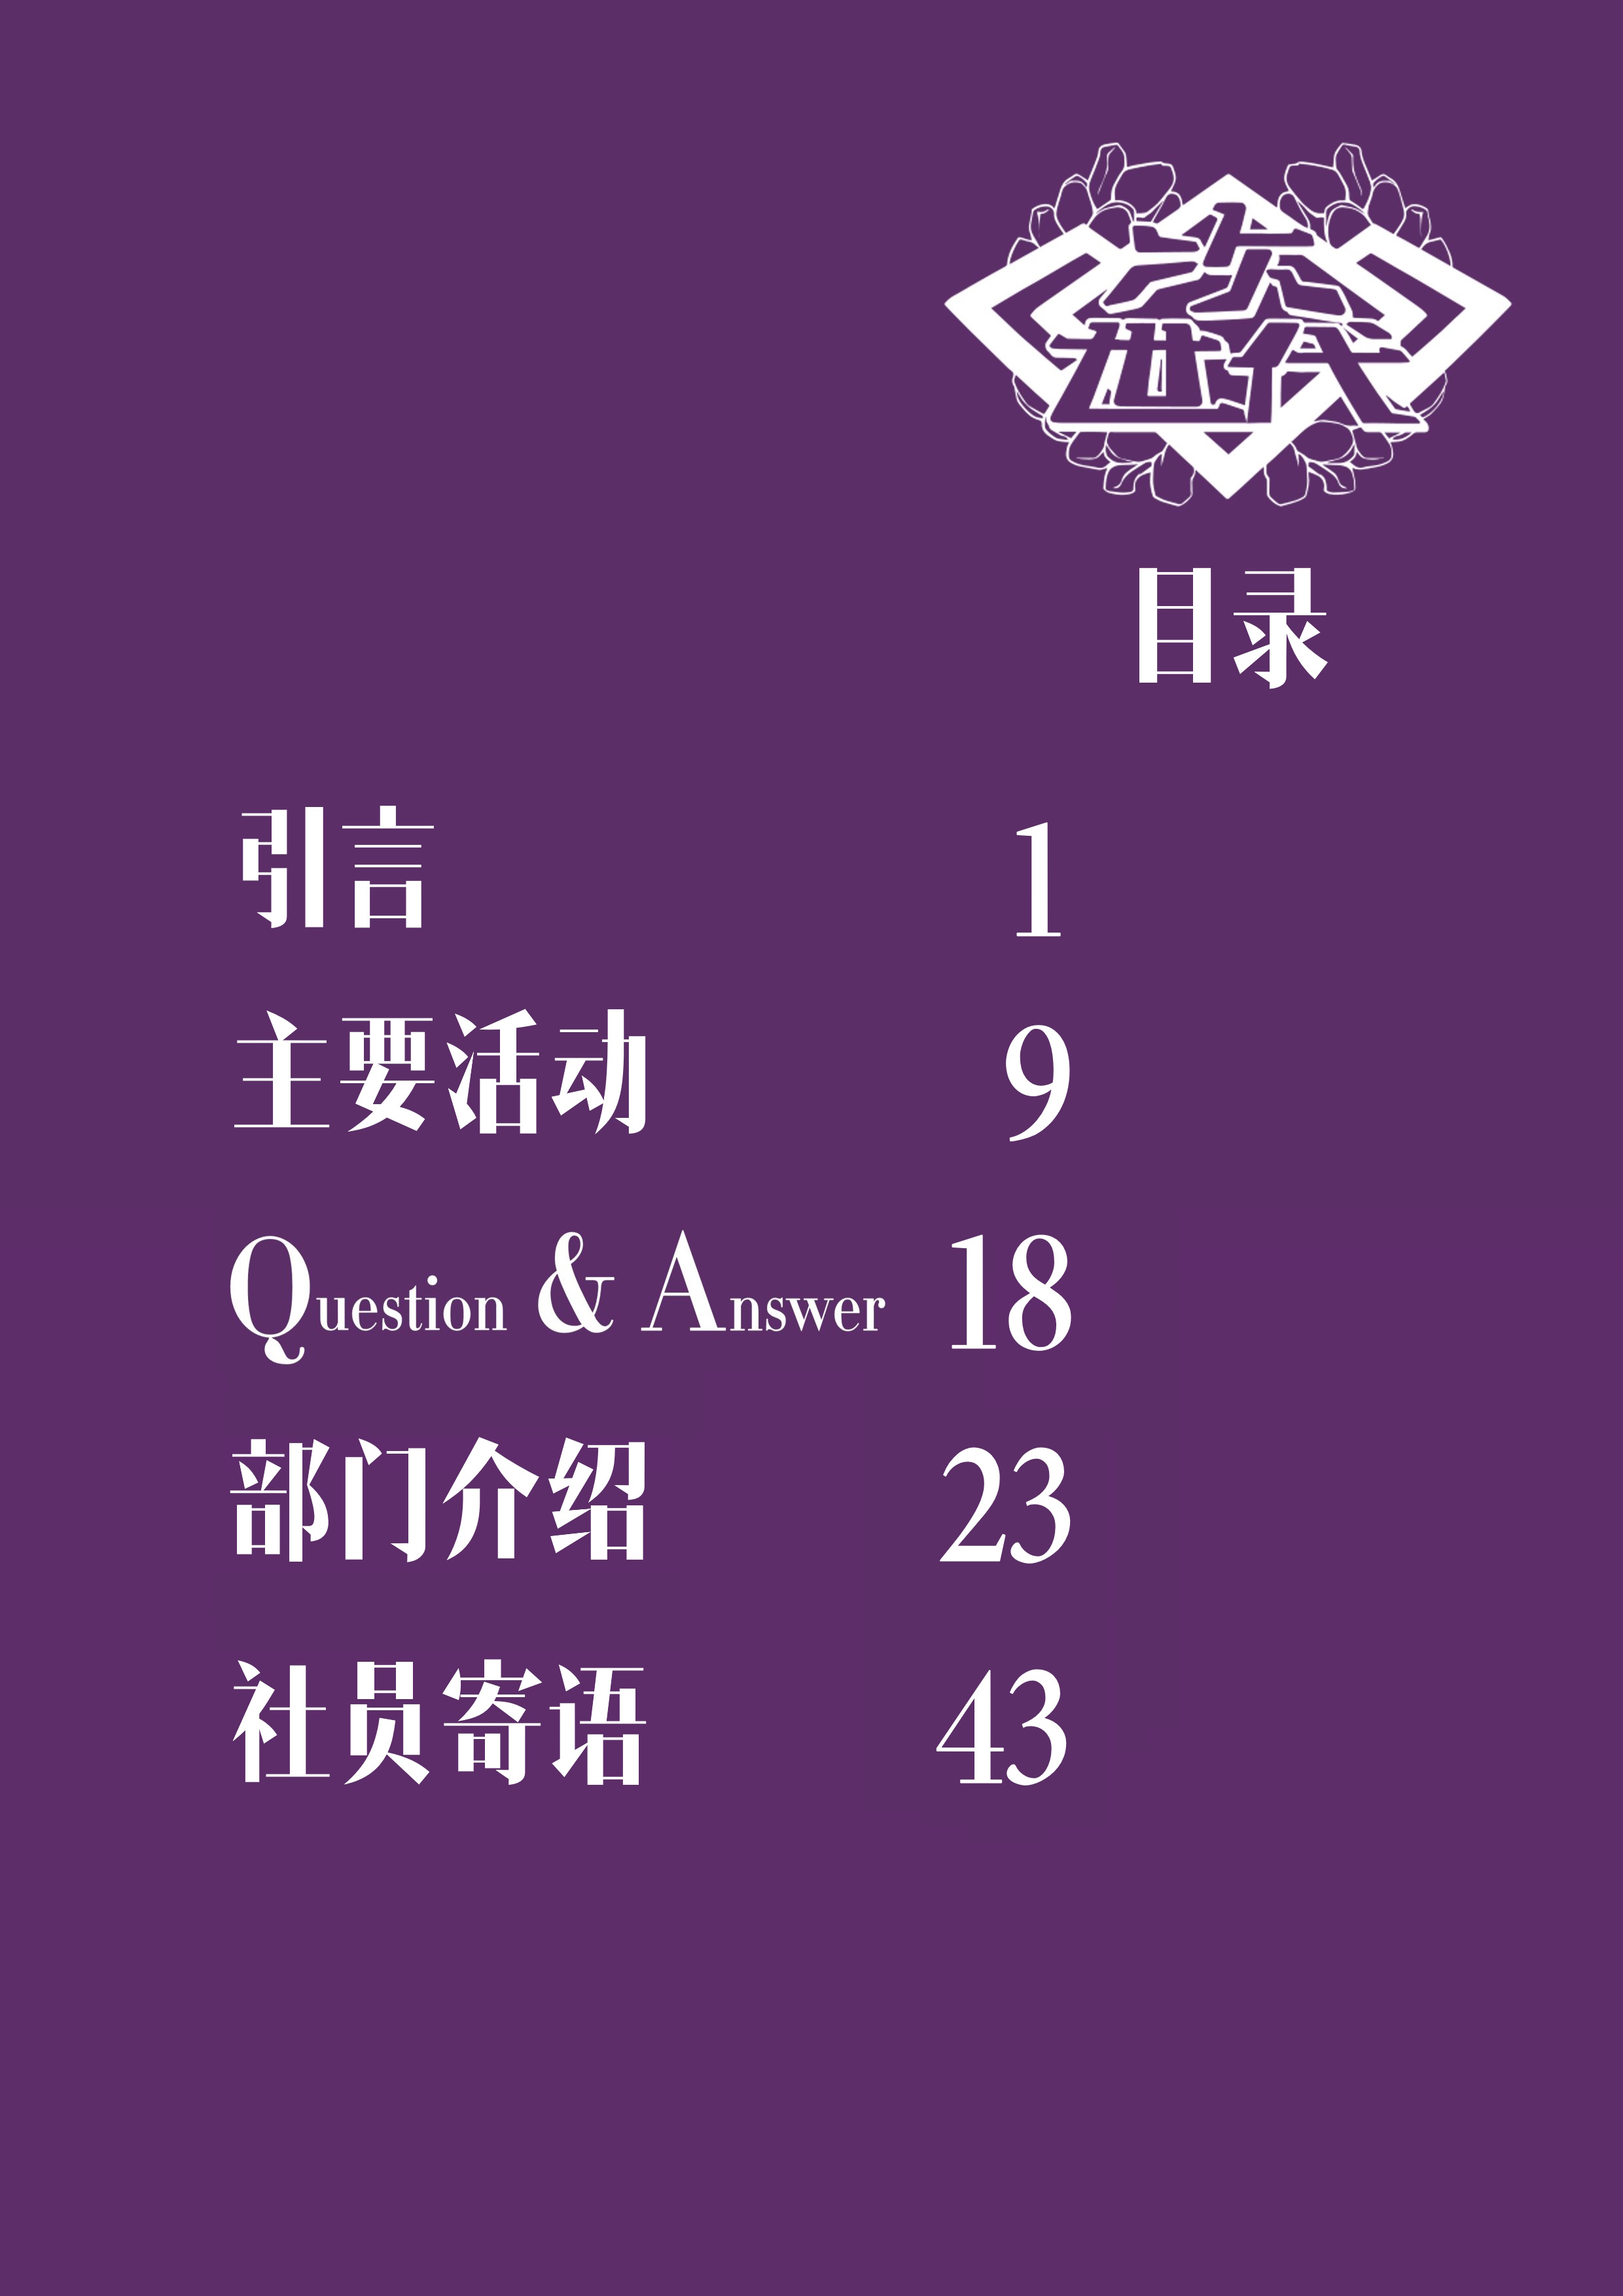
\includegraphics[width=0.9999\paperwidth, height=0.9999\paperheight]{ch1.jpg} % 插入图片,使其尺寸与纸张大小一致并保持宽高比[1](@ref)
    \restoregeometry % 恢复原来的页边距设置
\newpage
\begin{center}
    \fontsize{30pt}{32pt}\selectfont
    \textbf{\textcolor{truepurple}{部门全表}}  % 中文标题
    \\[0ex]  % 标题间距
    \fontsize{18pt}{20pt}\selectfont
    \textcolor{thuorange}{Department List}  % 英文标题
\end{center}
\flushleft  % 左对齐
\begin{multicols}{3}  % 三栏布局
    
    % 使用categorysection环境组织部门分类
    % 每个分类使用一个categorysection环境
    \begin{categorysection}{组织部门}  % 分类标题
        \item 次世代2024-2026组织部
    \end{categorysection}
    
    \begin{categorysection}{创作类}
        \item 次世代绘画部
        \item 次世代Cosplay\&舞台剧部
        \item 次世代音声部
        \item 次世代MAD部
        \item 次世代视觉系
    \end{categorysection}
    
    \begin{categorysection}{歌舞艺术类}
        \item 次世代宅舞部
        \item 次世代乐队部
        \item 次世代水木wota艺\\(光棒艺)部
        \item 次世代lolita部
        \item 次世代vocaloid部
        \item 次世代配音部
        \item 次世代舞台创造科
        \item 次世代草根妖怪乐团\\(乐器部)
        \item 次世代曲艺部
        \item 次世代华语金曲部
        \item 次世代J-pop音乐交流部
        \item 次世代伪音学习部
        \item 次世代声乐学习部\\(学唱歌部)
        \item 次世代电子音乐部
        
    \end{categorysection}
    
    \begin{categorysection}{综合类}
        \item 次世代Galgame部
        \item 次世代轻小说部
        \item 次世代漫研部
        \item 次世代动画研究会
        \item 次世代百合部
        \item 次世代BL部
        \item 次世代绘画部
        \item 次世代国产动画部
        \item 次世代文艺部
        \item 次世代网文部
        \item 次世代恋爱喜剧部
        \item 次世代游戏制作交流部
        \item 次世代放映部
        \item 次世代同人文部
        \item 次世代读书交流部
        \item 次世代furry部
        \item 次世代心憩部
        \item 次世代奇幻+异世界部
        \item 次世代美图部
    \end{categorysection}

    \begin{categorysection}{作品类}
        \item 次世代东方project部\\(2019年新群)
        \item 次世代LoveLive!部
        \item 次世代白色相簿2部
        \item 次世代命运石之门部
        \item 次世代魔法少女小圆部
        \item 次世代芳文社部
        \item 次世代jojo部
        \item 次世代BanG Dream!部
        \item 次世代偶像部\\(偶像大师、偶像声优)
        \item 次世代少女歌剧部
        \item 次世代龙族部
        \item 次世代鬼灭之刃部
        \item 次世代进击的巨人部
        \item 次世代叛逆的鲁鲁修部
        \item 次世代赤坂作品研究部\\(辉夜大小姐\&我推的孩子)
        \item 次世代路学研究基地\\(路人女主)
        \item 次世代IDOLiSH7部
        \item 次世代兽耳放送部
        \item 次世代某部\\(魔禁超炮科方AB)
        \item 次世代西尾维新同好会
        \item 次世代凉宫春日部
        \item 次世代银河英雄传说部
        \item 次世代Re0部
        \item 次世代间谍过家家部
        \item 次世代小绿和小蓝部
        \item 次世代孤独摇滚部
        \item 次世代猫猫虫部
        \item 次世代京阿尼部
        \item 次世代SCP部
        \item 次世代aph部
        \item 次世代柯南部
        \item 次世代拜年祭\&2233部
        \item 次世代Macross部
    \end{categorysection}

    \begin{categorysection}{游戏类}
        \item 次世代STEAM部
        \item 次世代dota2部
        \item 次世代FGO部
        \item 次世代舰C部
        \item 次世代日麻部
        \item 次世代TRPG跑团部
        \item 次世代音游部
        \item 次世代游戏王部
        \item 次世代游戏王决斗链接部
        \item 次世代主机游戏部
        \item 次世代明日方舟部
        \item 次世代华大联盟工坊\\(我的世界部)
        \item 次世代FF14部
        \item 次世代怪物猎人部
        \item 次世代碧蓝航线部
        \item 次世代崩崩崩部
        \item 次世代阴阳师部
        \item 次世代英雄联盟部
        \item 次世代shadowverse部
        \item 次世代shadowverse evolve
        \item 次世代桌游部
        \item 次世代舰R部
        \item 次世代星际部
        \item 次世代DNF部
        \item 次世代暖暖部
        \item 次世代手游MOBA部
        \item 次世代彩虹六号围攻部
        \item 次世代CSGO部
        \item 次世代EnsembleStars部
        \item 次世代万智牌部
        \item 次世代文明部
        \item 次世代梦100部
        \item 次世代轨迹部
        \item 次世代国产rpg部
        \item 次世代冒险岛部
        \item 次世代火纹部
        \item 次世代碧蓝幻想部
        \item 次世代公主链接部
        \item 次世代FTG部
        \item 次世代英雄无敌部
        \item 次世代Ingress XM研究所
        \item 次世代魔法记录部
        \item 次世代原神部
        \item 次世代战双帕弥什
        \item 次世代永远的7日之都
        \item 次世代元气骑士部
        \item 次世代动物森友会
        \item 次世代宝可梦部
        \item 次世代persona部
        \item 次世代小众手游部
        \item 次世代Wixoss部
        \item 次世代黑白双翼Wei$\beta$~Schwarz部
        \item 次世代少女前线部
        \item 次世代少女前线2追放部
        \item 次世代APEX部
        \item 次世代プロセカ部
        \item 次世代云图计划部
        \item 次世代RPG MAKER\\游戏部
        \item 次世代魂血狼环部
        \item 次世代赛马娘部
        \item 次世代无期迷途部
        \item 次世代深空之眼部
        \item 次世代星穹铁道部
        \item 次世代炼金工房部
        \item 次世代蔚蓝档案部
        \item 次世代红警交流群
        \item 次世代重返未来1999部
        \item 次世代月亮计划游戏部
        \item 次世代PTCG部
        \item 次世代逆水寒手游部
        \item 次世代斯普拉遁部
        \item 次世代坦克世界部
        \item 次世代卡拉比丘部
        \item 次世代heaven burns red部
        \item 次世代rougelike部
        \item 次世代植物大战僵尸部
        \item 次世代物华弥新部
        \item 次世代duckgame部
        \item 次世代泰拉瑞亚部
        \item 次世代鸣潮
        \item 次世代绝区零
        \item 次世代p社游戏
        \item 次世代尘白禁区
        \item 次世代forza horizon
        \item 次世代VRChat部
        \item 次世代逆转裁判部
        \item 次世代EVE Online部
        \item 次世代第五人格部
        \item 次世代rimworld/环世界部
        \item 次世代新月同行部
        \item 次世代戴森球计划部
        \item 次世代绝地潜兵部
        \item 次世代火影忍者手游部
        \item 次世代JRPG部
        \item 次世代csgo菜鸟部
        \item 次世代战锤部
        \item 次世代剑三部
        \item 次世代三角洲行动部
        \item 次世代银与绯
        \item 次世代夜幕魅影
        \item 次世代星露谷物语部
        \item 次世代都市天际线部
        \item 次世代米游杂食铺
    \end{categorysection}

    \begin{categorysection}{娱乐影视类}
        \item 次世代Vtuber单推部
        \item 次世代男声优部
        \item 次世代女声优部
        \item 次世代三次元偶像部
        \item 次世代地下偶像部
        \item 次世代电影电视剧部
        \item 次世代特摄部
        \item 次世代大友部
        \item 次世代asmr部
        \item 次世代动画歌牌部
        \item 次世代华清魔法部
        \item 次世代神椿深脊少革部
    \end{categorysection}

    \begin{categorysection}{科技生活类}
        \item 次世代打工部
        \item 次世代外卖部
        \item 次世代硬件部
        \item 次世代电子系部\\(电子系互助部)
        \item 次世代数学部
        \item 次世代学习部
        \item 次世代日本分部
        \item 次世代运动部
        \item 次世代足球部
        \item 次世代手办种草部
        \item 次世代火锅部
        \item 次世代养生部
        \item 次世代3D建渲部
        \item 次世代双清部(双清公寓)
        \item 次世代AI绘画部
        \item 次世代机器学习部
        \item 次世代跑路军团(旅行部)
        \item 次世代对抗脱发部
        \item 次世代猫猫部
        \item 次世代社畜群
        \item 次世代篮球部
        \item 次世代f1部
        \item 次世代色觉异常部
        \item 次世代机航动抱团互助部
        \item 次世代Kigurumi部
        \item 次世代软件开发部
        \item 次世代日语学习部
        \item 次世代中古部
        \item 次世代语言学部
        \item 次世代多邻国部
        \item 次世代摄影部
        \item 次世代小厨娘部\\(烹饪/晒饭部)
        \item 次世代道具制造部
        \item 次世代周边交易部(谷子部)
    \end{categorysection}

\end{multicols}
\newpage
% }}}
\begin{flushleft}
  \adjustbox{valign=t}{
    \begin{minipage}[t]{0.35\textwidth}
      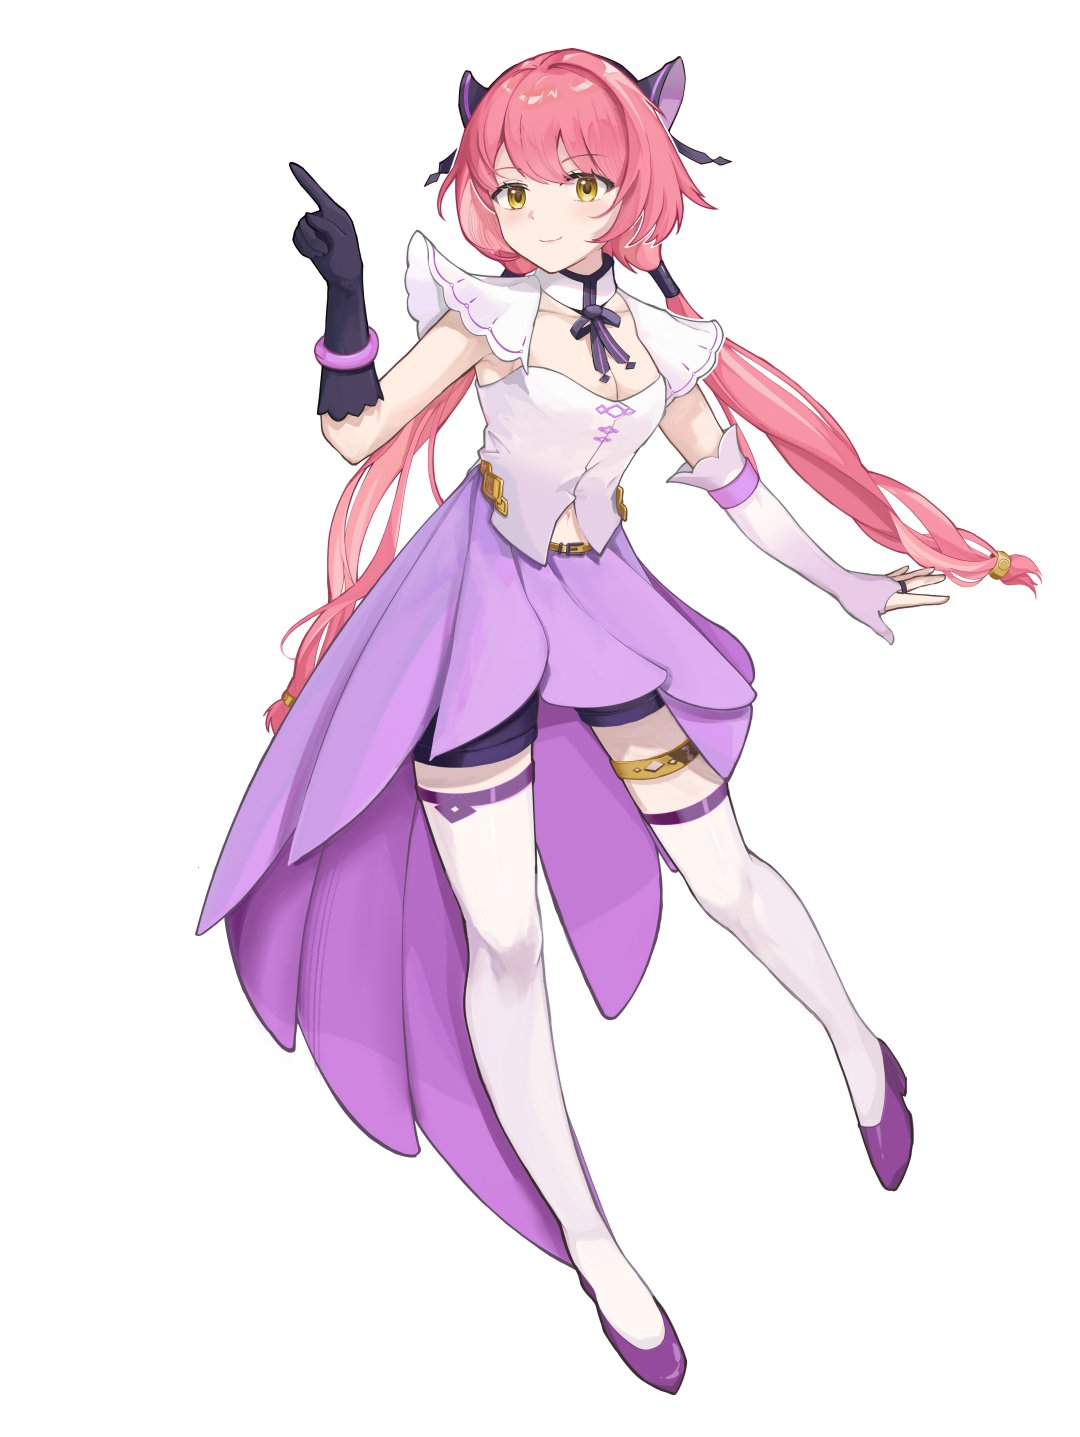
\includegraphics[width=\linewidth]{taozifull.jpg}
    \end{minipage}%
    }
    \hfill
    \adjustbox{valign=t}{
    \begin{minipage}[t]{0.55\textwidth}
        \vspace{10pt}
        \section*{\Large\textbf{\textcolor{taopink}{桃子}}}
        \vspace{-1em}
        \subsection*{\normalsize\textbf{\textcolor{thuorange}{Meet Taozi}}}
        \vspace{-0em}
        \small
        \chind 作为大家公认的金牌吃货,最喜欢和大家一起分享校内外好吃的东西,
        最近最喜欢的食物是清芬亲手做的点心;同时也作为大家公认的电脑白痴,
        几乎每周都要上演《我什么都没做电脑就坏了》的经典桥段……\\
        \chind 最喜欢紫哥和清芬,
        并且毫不掩饰自己的感情,有时候也会配合清芬一起捉弄紫哥;同时也最喜欢次世代的大家,
        目前正在和清芬一起努力,希望成为次世代大家心目中最可爱的偶像!
        \vspace{0.4em}
    \end{minipage}
    }
\end{flushleft}
\begin{flushleft}

    \adjustbox{valign=t}{
    \begin{minipage}[t]{0.55\textwidth}
        
        \section*{\Large\textbf{\textcolor{truepurple}{紫荆}}}
        \vspace{-1em}
        \subsection*{\normalsize\textbf{\textcolor{thuorange}{Meet Zijing}}}
        \vspace{-0em}
        \small
        \chind 作为次世代大家心照不宣的无口系+暖男系+亚撒西帅哥,
        被大家亲切地称为“紫哥”,家务做饭、电器维修、电子游戏全能的紫哥
        也成为了桃子最为依赖的存在;但是紫荆在运动方面却惊人地残念,
        明明拥有那么好的身材……都系得(\\
        \chind 作为大家最喜欢的长辈(?),
        虽然常常被清芬和桃子捉弄,但是却从未生过气;很擅长保护桃子和清芬,
        同时也视她们为生命中最需要守护的存在,而这一理念带来的结果就是紫荆
        常常会无意识地对桃子和清芬进行说教,
        结果往往引来她俩新一轮的捉弄,真是无奈啊……
        \vspace{0.4em}
        \vspace{\baselineskip}
    \end{minipage}
    }
    \hfill
  \adjustbox{valign=t}{
    \begin{minipage}[t]{0.35\textwidth}
      \vspace{-4em}
      \raisebox{-\height}[0pt][0pt]{
      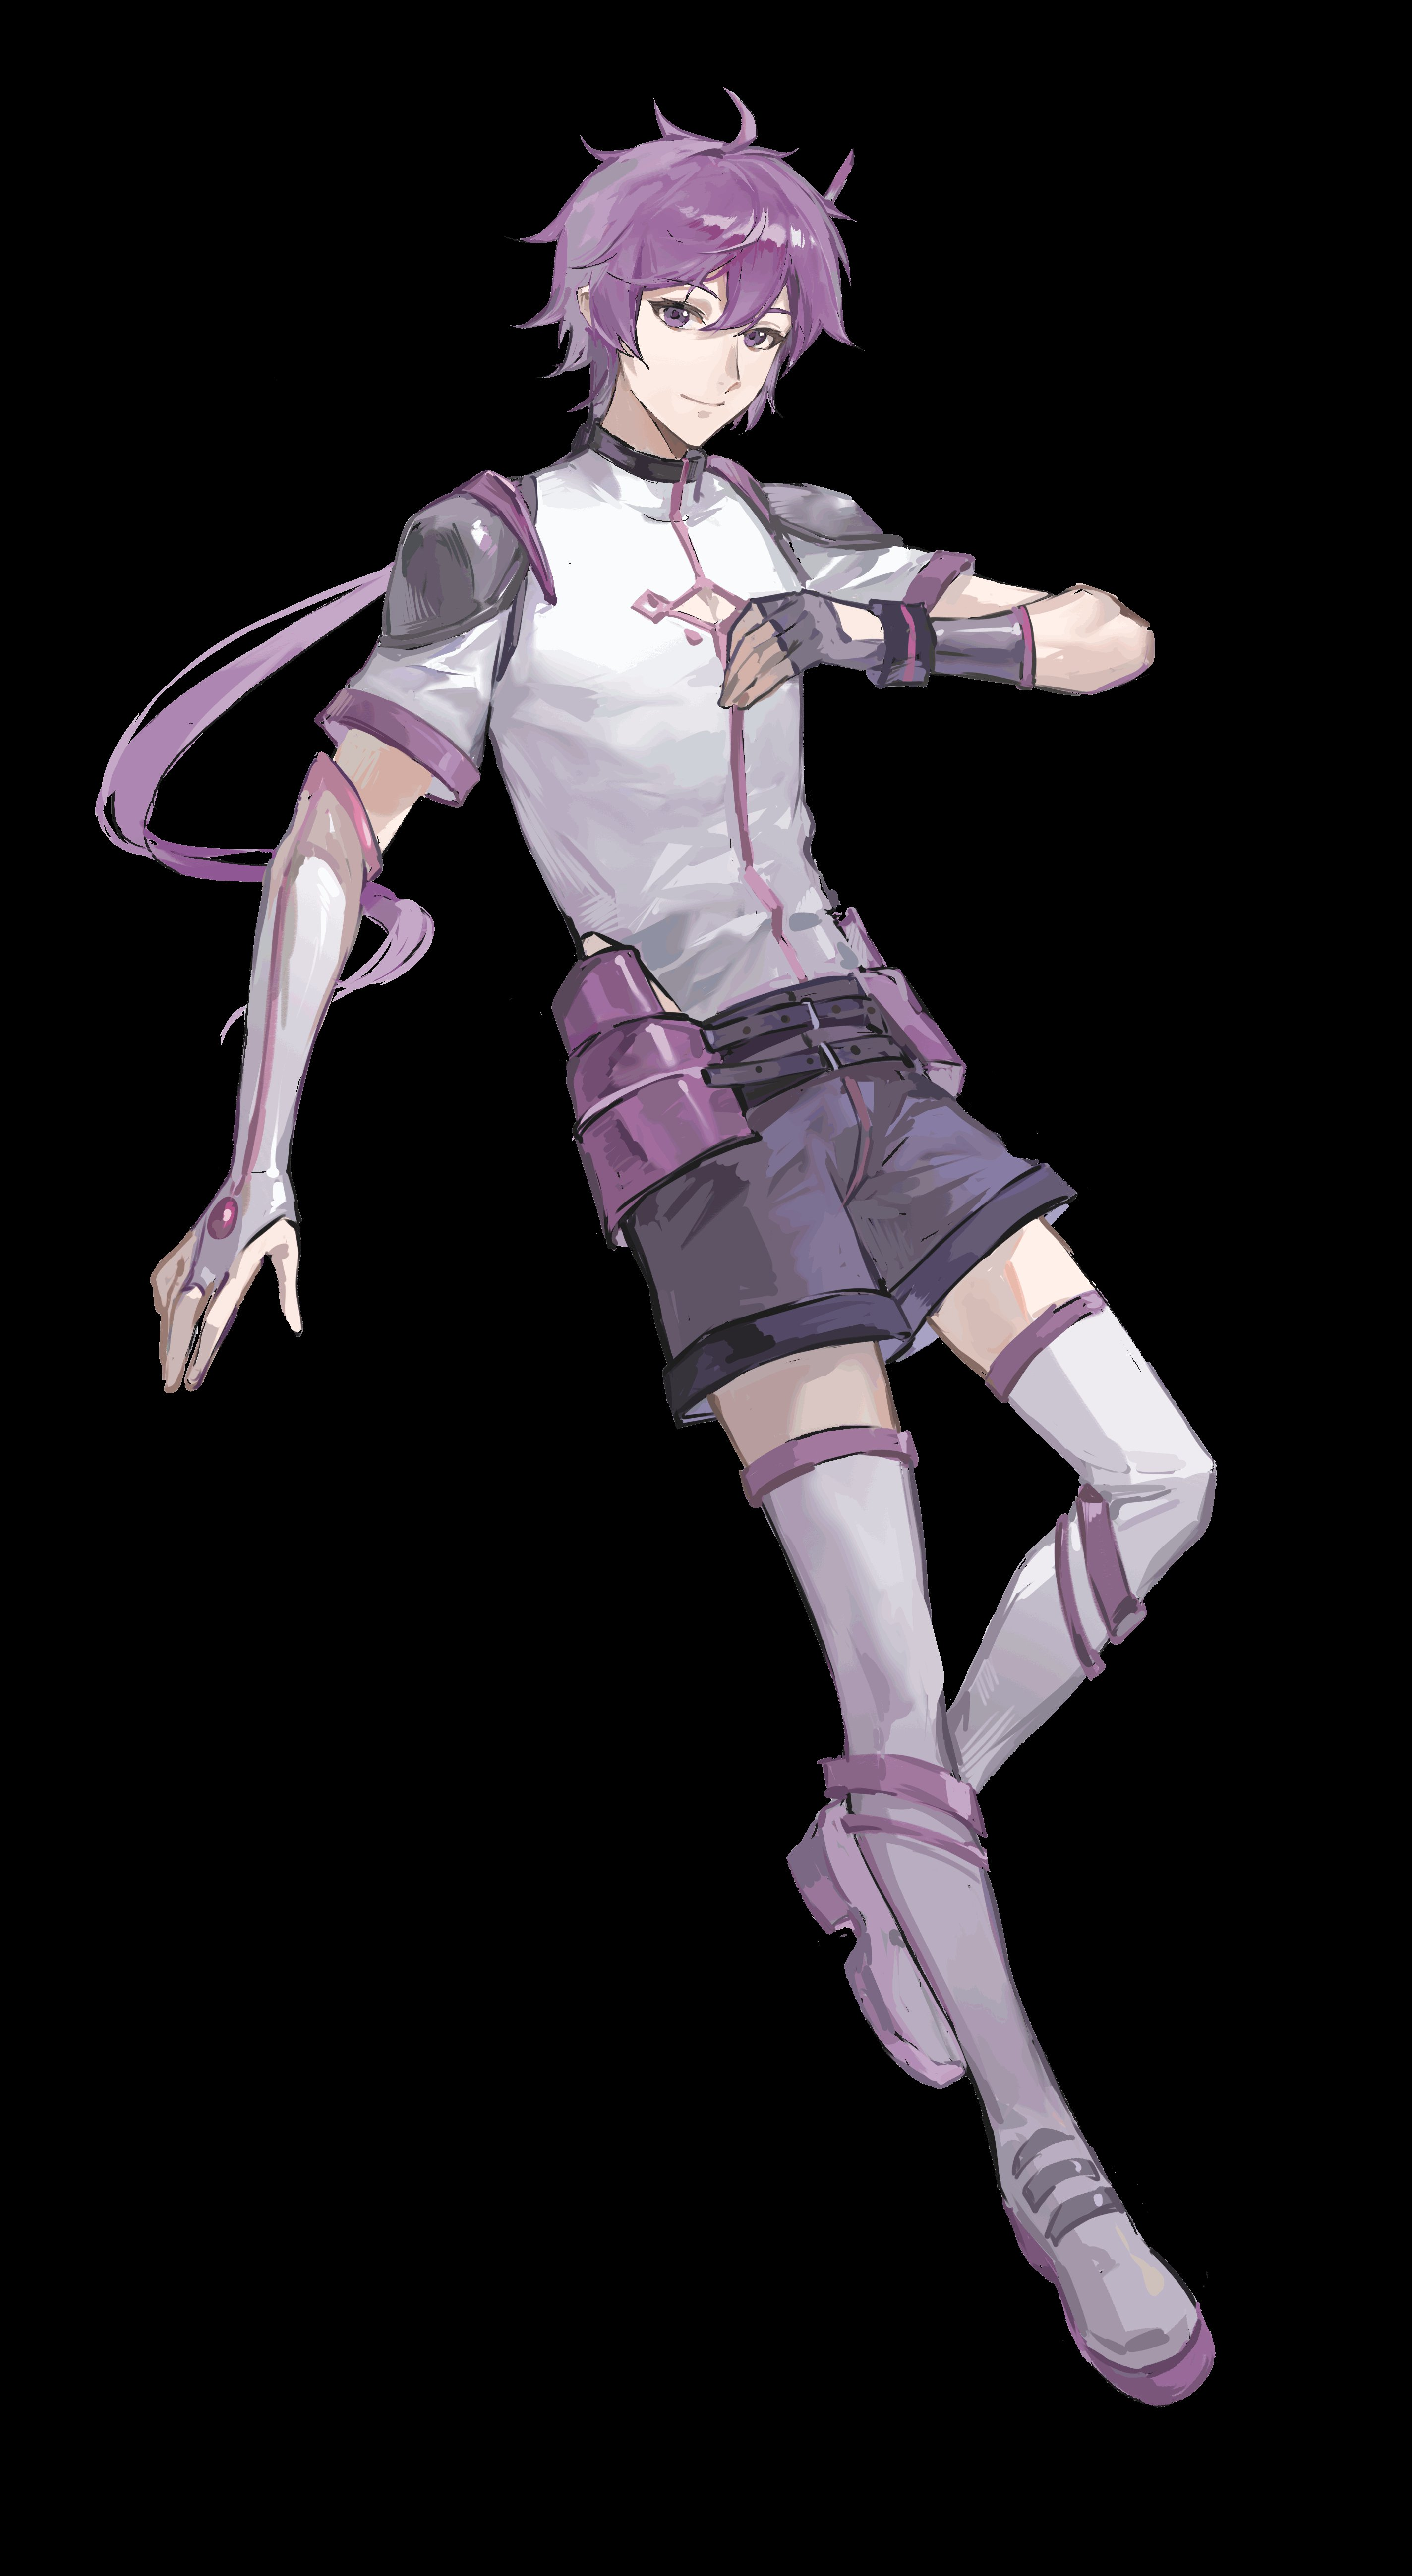
\includegraphics[height=1.82\linewidth,width=\linewidth]{zijingfull.jpg}}
    \end{minipage}%
    }
    
  
\end{flushleft}

  \adjustbox{valign=t}{
    \begin{minipage}[t]{0.35\textwidth}
      \vspace{-2em}
      \raisebox{-\height}[0pt][0pt]{
      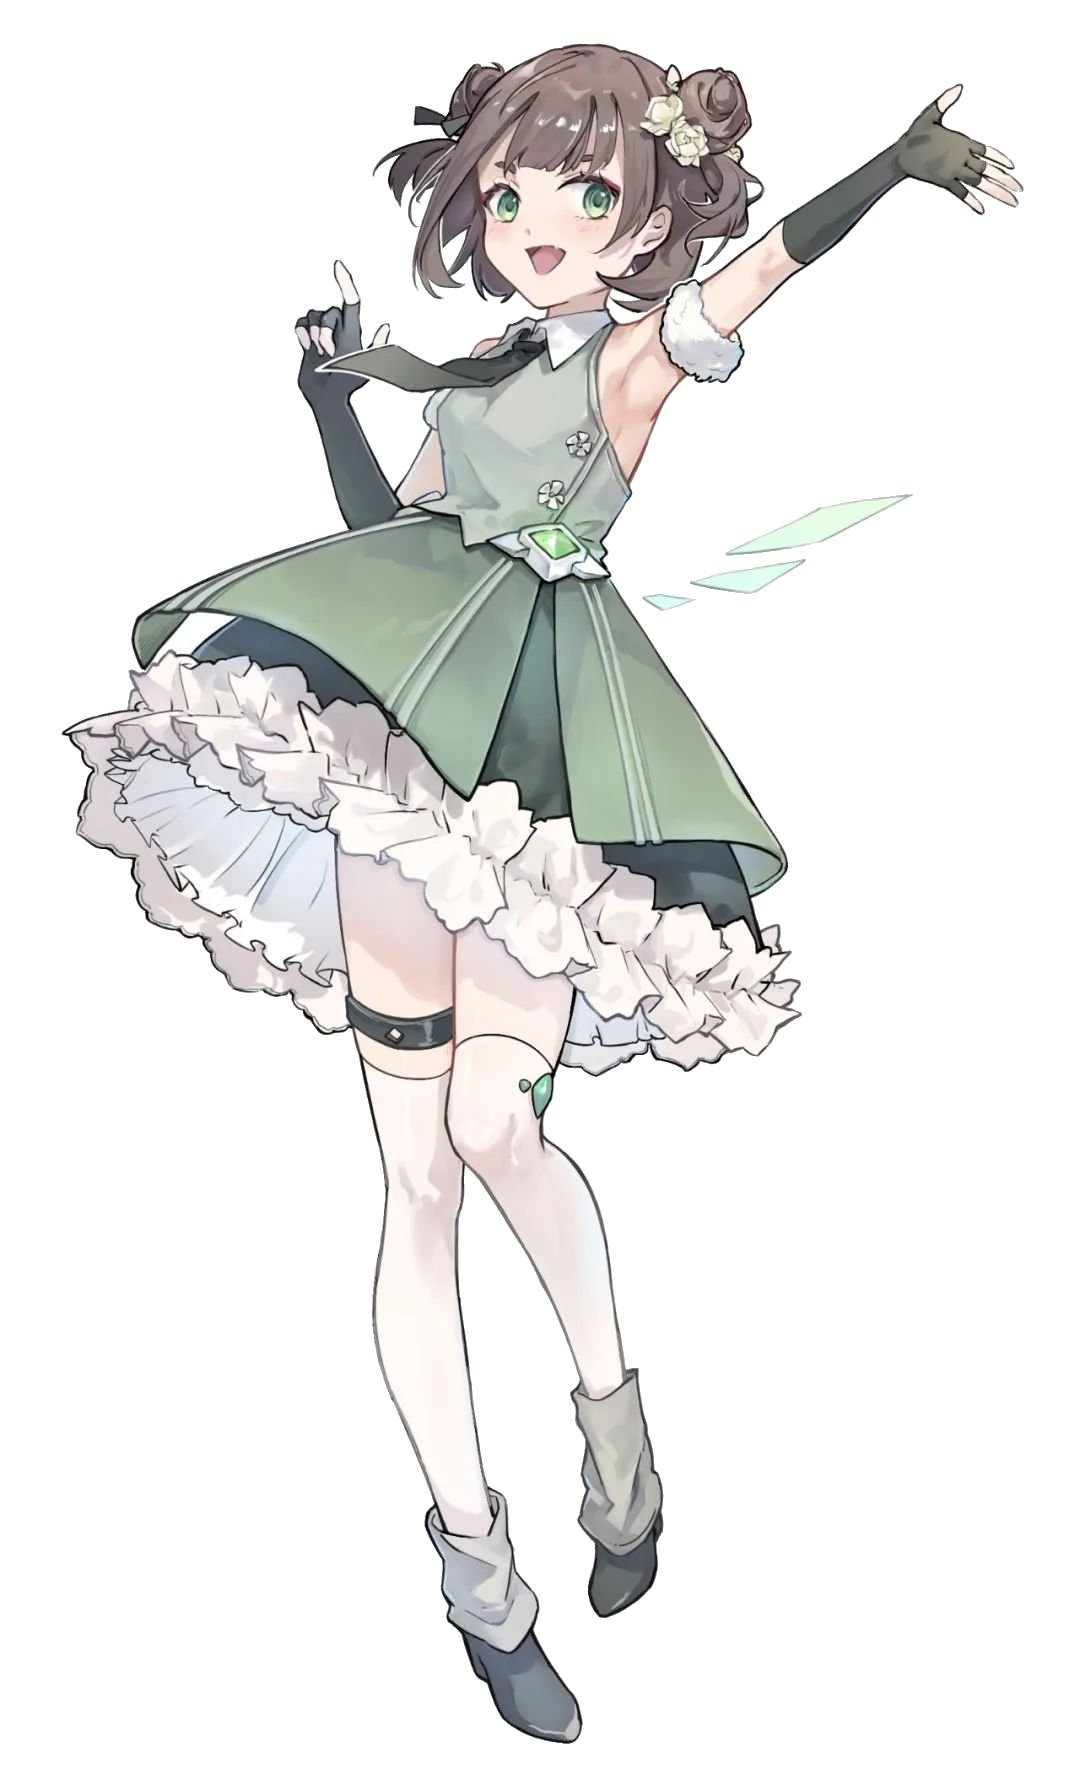
\includegraphics[width=0.85\linewidth]{qingfenfull.jpg}}
    \end{minipage}%
    }
    \hfill
    \adjustbox{valign=t}{
    \begin{minipage}[t]{0.55\textwidth}
        \section*{\Large\textbf{\textcolor{green!50!black}{清芬}}}
        \vspace{-1em}
        \subsection*{\normalsize\textbf{\textcolor{thuorange}{Meet Qingfen}}}
        \vspace{-0em}
        \small
      \chind 自幼便能歌善舞、希望带给大家开心和笑容的清芬加入次世代大家庭后,
      马上成为了社友们眼中最闪耀的偶像!\\ 
      \chind 作为次世代最小的看板娘,
      非常喜欢桃子和紫哥(虽然常常以玩笑掩饰自己的这份喜欢)。平时尤以捉弄桃子为乐,但是又会做非常多超好吃的甜点带给桃子,
      引得桃子对清芬死心塌地(?);\\ 
      \chind 日常中欢快跳脱的性格
      和舞台上闪闪发光的演出引得众人喜爱,
      但是也常常做出种种脱线的行为,让紫哥头疼不已……    
        \vspace{0.4em}
    \end{minipage}
    }
% 聊天对话部分
% 使用chatbubble命令创建对话气泡
% 语法:\chatbubble[位置]{头像}{昵称}{内容}{背景色}
\newpage 
\chatbubble[left]{taozi.jpg}{桃子没有在摸鱼}{%
大家好,这里是次世代的初代看板娘桃子\~{}
}{tao}
\chatbubble[left]{qingfen.jpg}{清芬哒哟}{%
大家好!我是次世代的看板娘清芬!
}{qing}
\chatbubble[right]{zijing.jpg}{紫荆}{
  我是紫荆。
}{zi}
\chatbubble[left]{taozi.jpg}{桃子没有在摸鱼}{%
那么什么是次世代呢?
}{tao}
\chatbubble[right]{zijing.jpg}{紫荆}{
那么什么是次世代呢?
}{zi}
\chatbubble[left]{qingfen.jpg}{清芬哒哟}{%
客服工号1911桃子为您解答:
}{qing}
\chatbubble[left]{taozi.jpg}{桃子没有在摸鱼}{%
?!
}{tao}
\chatbubble[left]{taozi.jpg}{桃子没有在摸鱼}{%
欸多\~{}咳嗯!次世代全称清华大学学生次世代动漫社,是,是……由两百多个兴趣部门组成的……
}{tao}
\chatbubble[left]{qingfen.jpg}{清芬哒哟}{%
……泛ACGN类兴趣社团(看稿子)
}{qing}
\chatbubble[right]{zijing.jpg}{紫荆}{
你俩……
}{zi}
\chatbubble[left]{taozi.jpg}{桃子没有在摸鱼}{%
咳嗯!次世代的一大特色就是丰富多彩的兴趣部门。从ACGN到运动养生,无论你对什么感兴趣,都可以在分部里找到你的同好!
}{tao}
\chatbubble[left]{qingfen.jpg}{清芬哒哟}{%
是的!即使没有找到组织,也可以秉着“三人成部”的原则,寻找同好,建立自己的兴趣部门!目前已经注册在案的有两百多个部门了\~{}
}{qing}
\chatbubble[right]{zijing.jpg}{紫荆}{
言归正传。接下来,让我们看一些社团资料,更加深入地了解次世代。
}{zi}
\newpage  % 第一章:社团介绍
\clearpage
\newpage % 开始新的一页
     % 移除本页的页眉和页脚[8,9](@ref)
    \newgeometry{margin=0pt} % 临时将本页的页边距全部设置为0[1](@ref)
    \noindent % 防止缩进
    
\includegraphics[width=0.9999\paperwidth, height=0.9999\paperheight]{ch2.jpg} % 插入图片,使其尺寸与纸张大小一致并保持宽高比[1](@ref)
    \restoregeometry % 恢复原来的页边距设置

\newpage
\newpage
\fontsize{23pt}{24pt}\selectfont
\begin{center}
    \textbf{\textcolor{truepurple}{百团大战\&迎新晚会}}\\
\end{center}
\vspace{0.7em}
\adjustbox{valign=t}{
	\begin{minipage}[t]{0.45\textwidth}
		\normalsize
		\chind 一年两度,次世代的大家拿出自己最大的热情欢迎新朋友!\\
    \chind 我们一直是百团最热闹的摊位之一。有各位同学自发贡献展示的手办、周边、图书展出;来自绘画部画师们的现场签绘、互绘;乐队部带来的现场演奏;cosplay舞台剧部的coser聚会、宅舞部献上的随舞表演;以及随后的wota艺节目……是招新,也是借机团建!\\
    \chind 在百团之后,我们会举办迎新晚会,进行各个分部的介绍展示与好玩的一站到底环节。\\
  		\par
		\vspace{-1em}
		\raisebox{-\height}{
			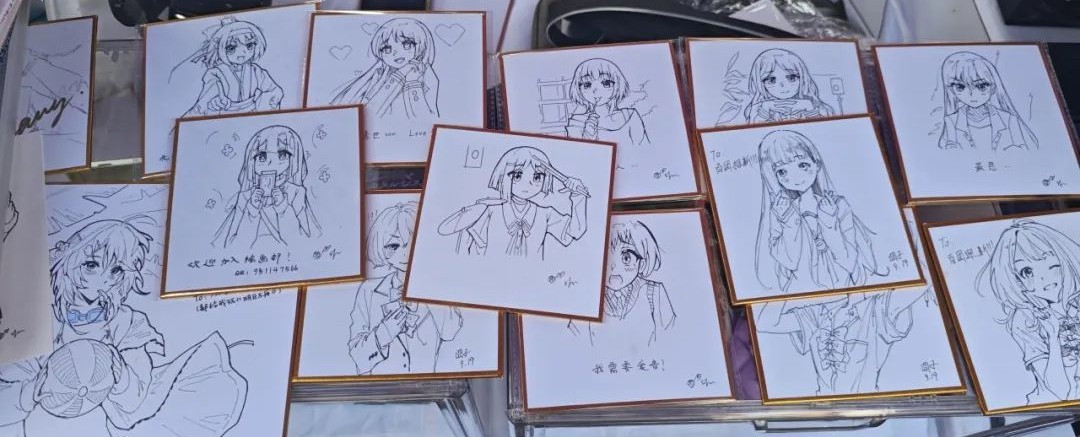
\includegraphics[width=\linewidth]{百团4.jpg}}
		\vspace{-0.5em}
		\picbox{\small ~\ding{115} ~ 绘画部现场签绘~}
		\par
		\vspace{-1em}
		\raisebox{-\height}{
			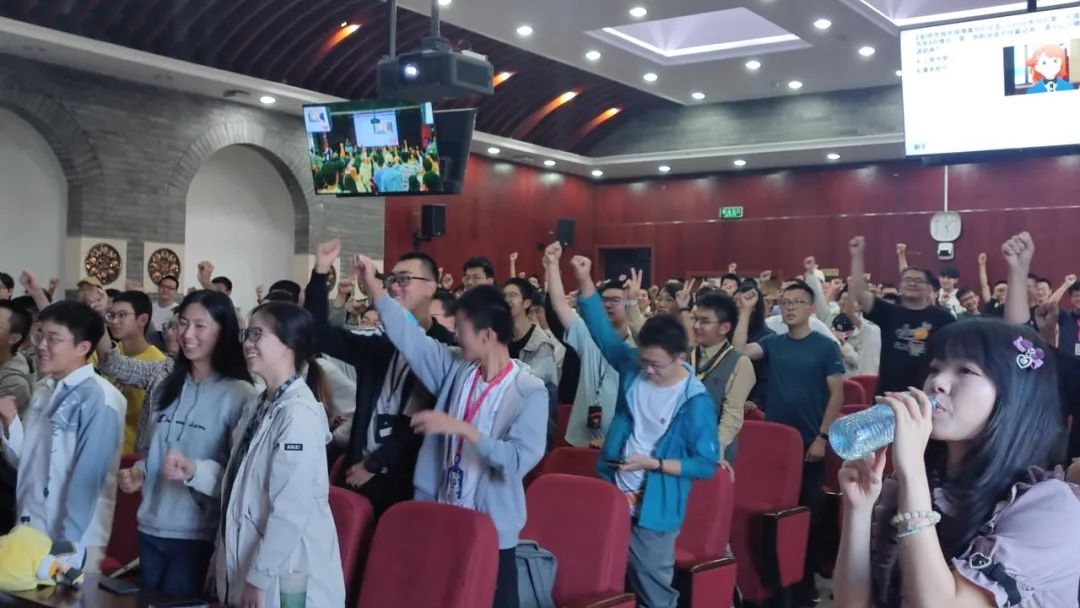
\includegraphics[width=\linewidth]{百团3.jpg}}
		\vspace{-0.5em}
		\picbox{\small ~\ding{115} ~ 一站到底~}
	\end{minipage}}
\hfill
\vspace{1em}
\adjustbox{valign=t}{
	\begin{minipage}[t]{0.45\textwidth}
		\vspace{-0.5em}
		\raisebox{-\height}{
			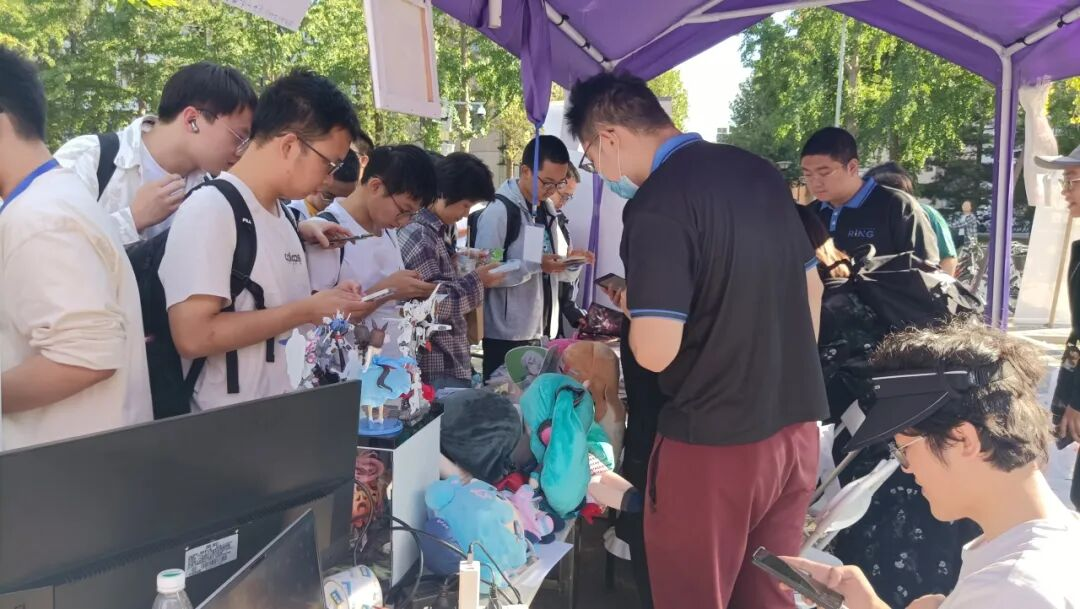
\includegraphics[width=\linewidth]{百团1.jpg}}
		\vspace{-0.5em}
		\picbox{\small ~\ding{115} ~ 走\scriptsize\sout{错}\normalsize\textbf{对}大学第一步~}
		\par
		\vspace{-1em}
		\raisebox{-\height}{
			
\includegraphics[width=\linewidth]{百团2.jpg}}
		\vspace{-0.5em}
		\picbox{\small ~\ding{115} ~ 随机宅舞~}
		\par
		\vspace{-1em}
		\raisebox{-\height}{
			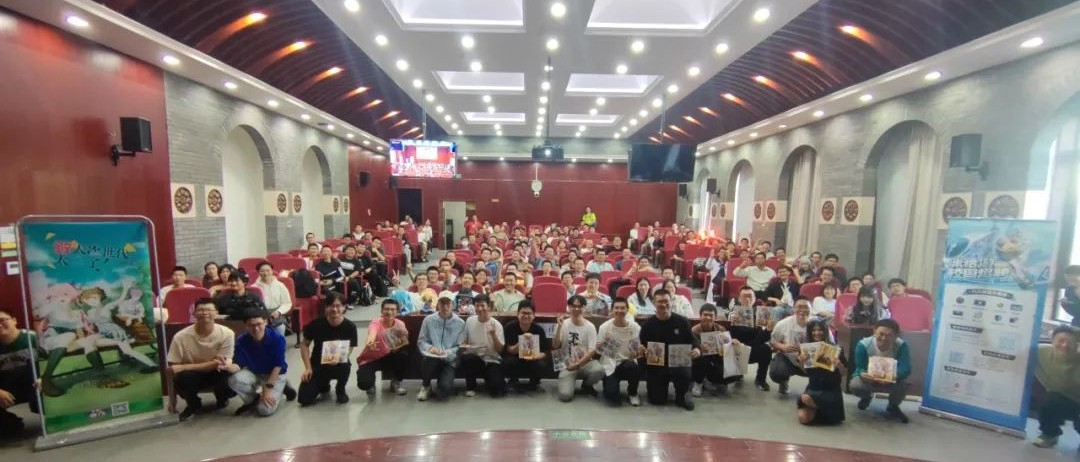
\includegraphics[width=\linewidth]{百团5.jpg}}
		\vspace{-0.5em}
		\picbox{\small ~\ding{115} ~ 迎新晚会合影~}
	\end{minipage}%
}
\begin{textblock*}{\paperwidth}(0mm, \dimexpr\paperheight-78.5mm\relax) % 距顶部 = 纸高 - 30mm
  \noindent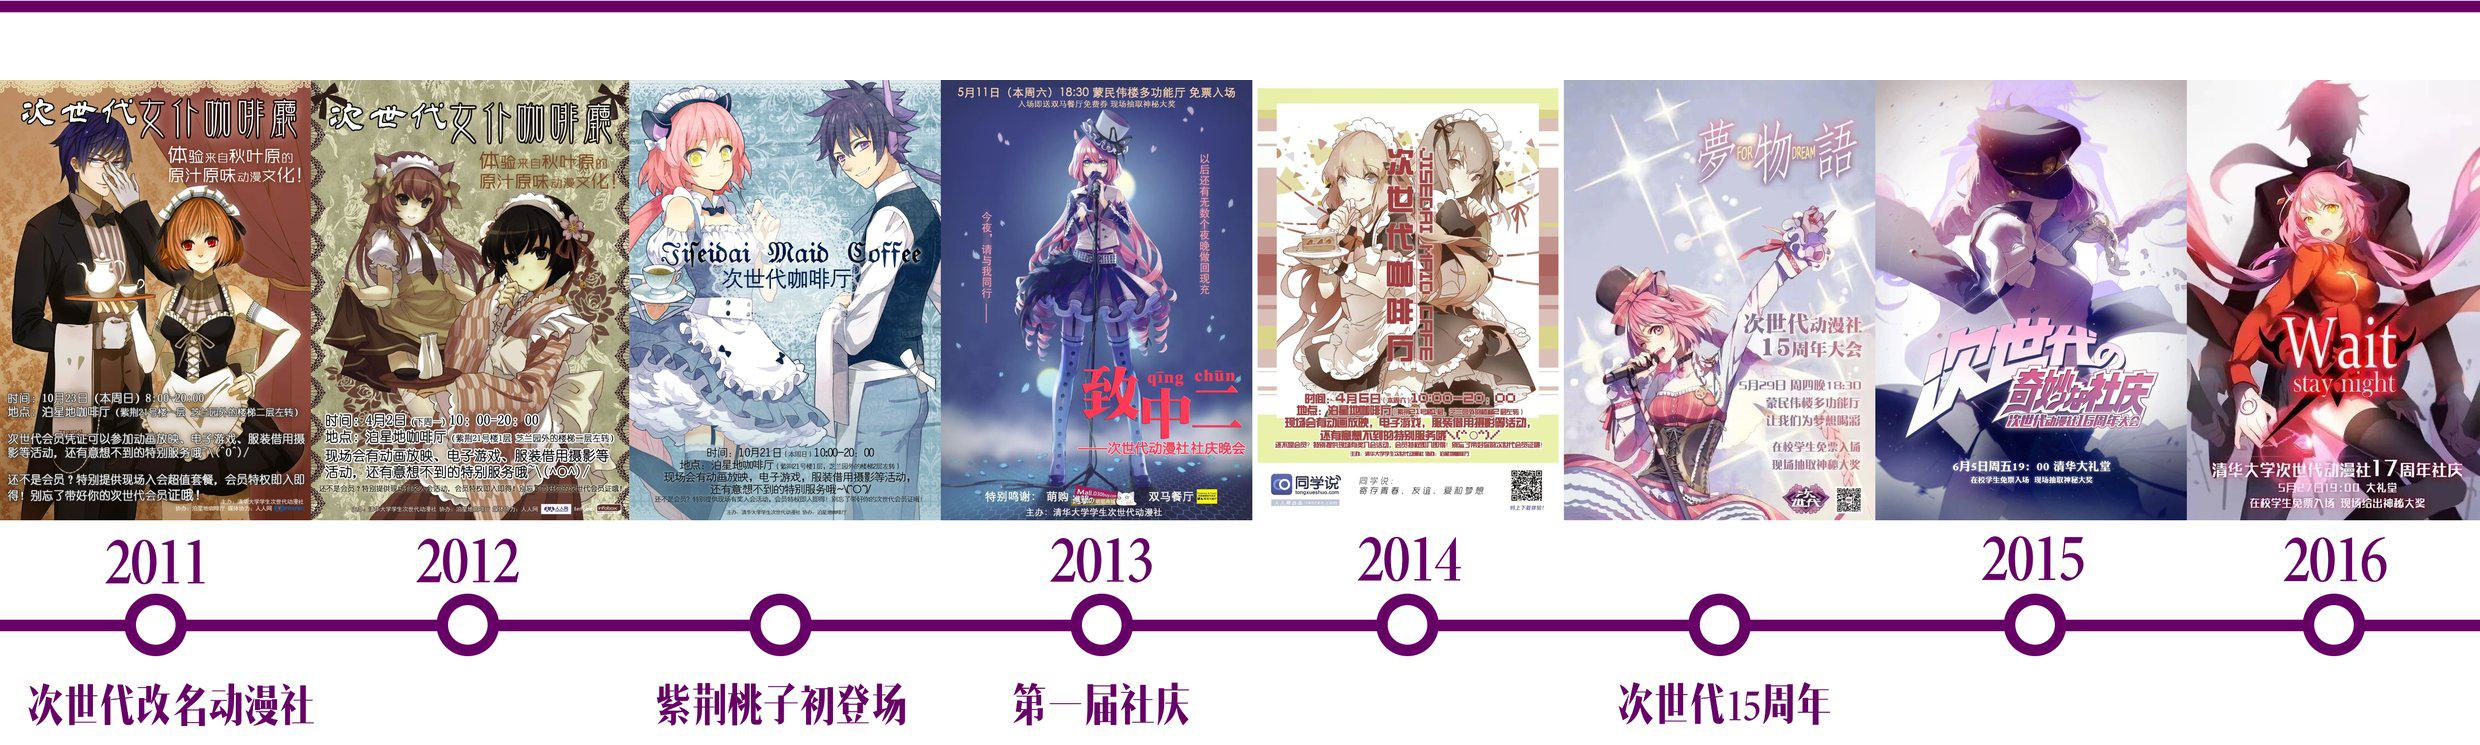
\includegraphics[width=\paperwidth]{tl1.jpg}
\end{textblock*}



\newpage
\fontsize{23pt}{24pt}\selectfont
\begin{center}
    \textbf{\textcolor{truepurple}{动漫主题咖啡厅}}\\
\end{center}
\vspace{0.7em}
\adjustbox{valign=t}{
	\begin{minipage}[t]{0.45\textwidth}
		\vspace{-0.5em}
		\raisebox{-\height}{
			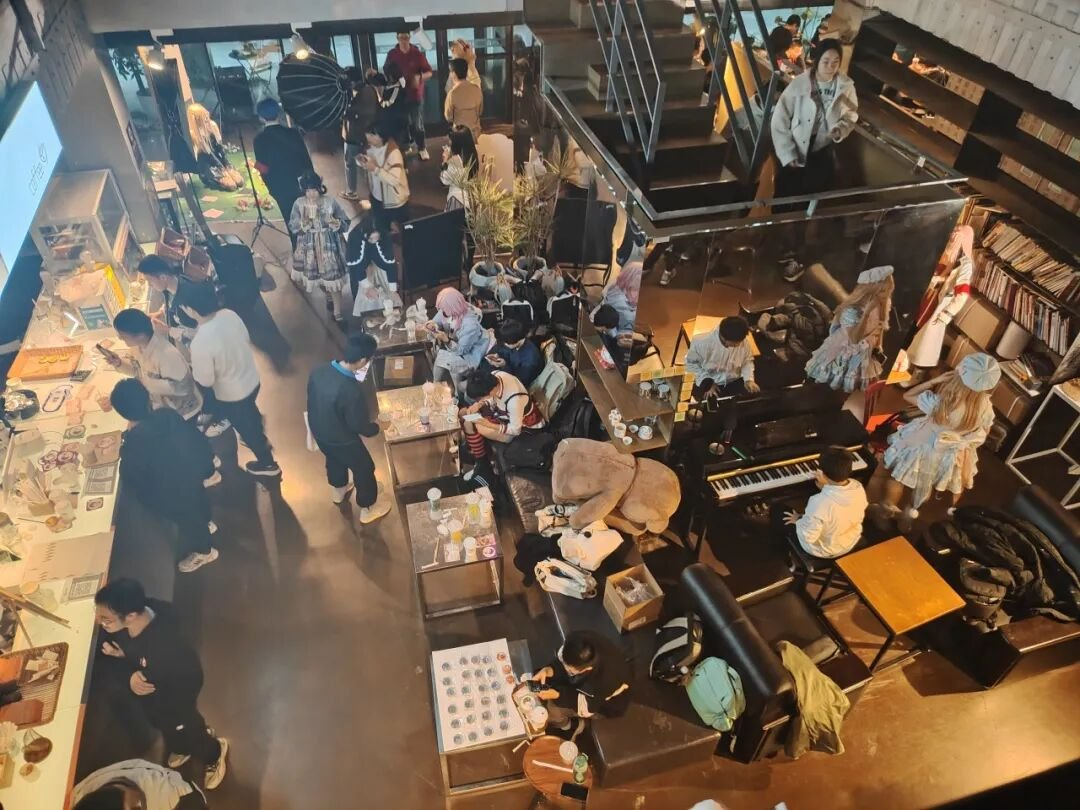
\includegraphics[width=0.9\linewidth]{咖啡厅3.jpg}}
		\vspace{-0.5em}
		\picbox{\small ~\ding{115} ~ 咖啡厅全景~}
  		\par
		\vspace{-1em}
		\raisebox{-\height}{
			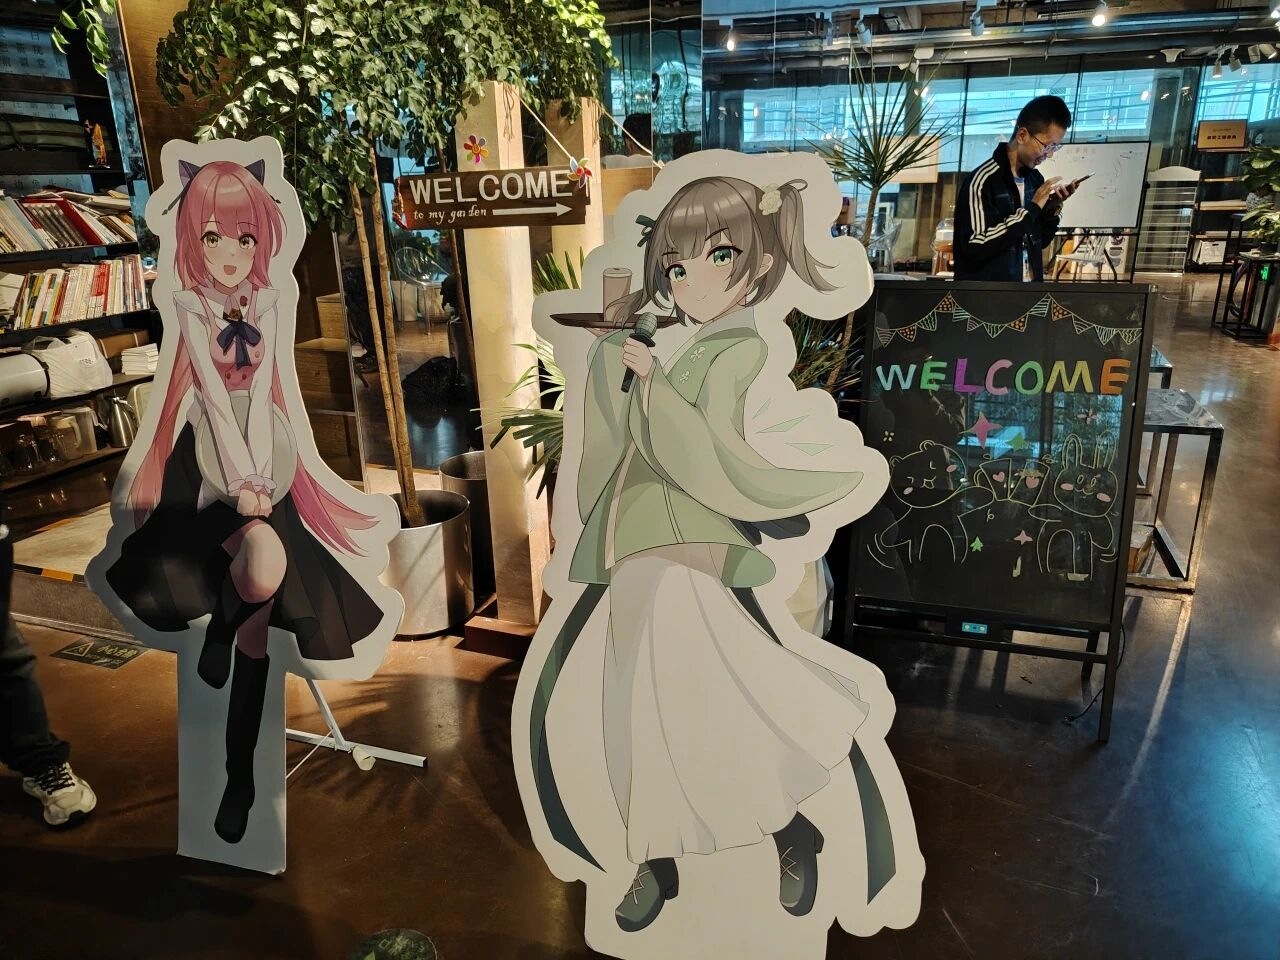
\includegraphics[width=0.9\linewidth]{咖啡厅2.jpg}}
		\vspace{-0.5em}
		\picbox{\small ~\ding{115} ~ 看板营业中~}
		\par
		\vspace{-1em}
		\raisebox{-\height}{
			\includegraphics[width=0.9\linewidth]{咖啡厅1.jpg}}
		\vspace{-0.5em}
		\picbox{\small ~\ding{115} ~ coser合影~}
	\end{minipage}}
\hfill
\vspace{1em}
\adjustbox{valign=t}{
	\begin{minipage}[t]{0.45\textwidth}

		\par
    \vspace{-0.5em}
		\raisebox{-\height}{
			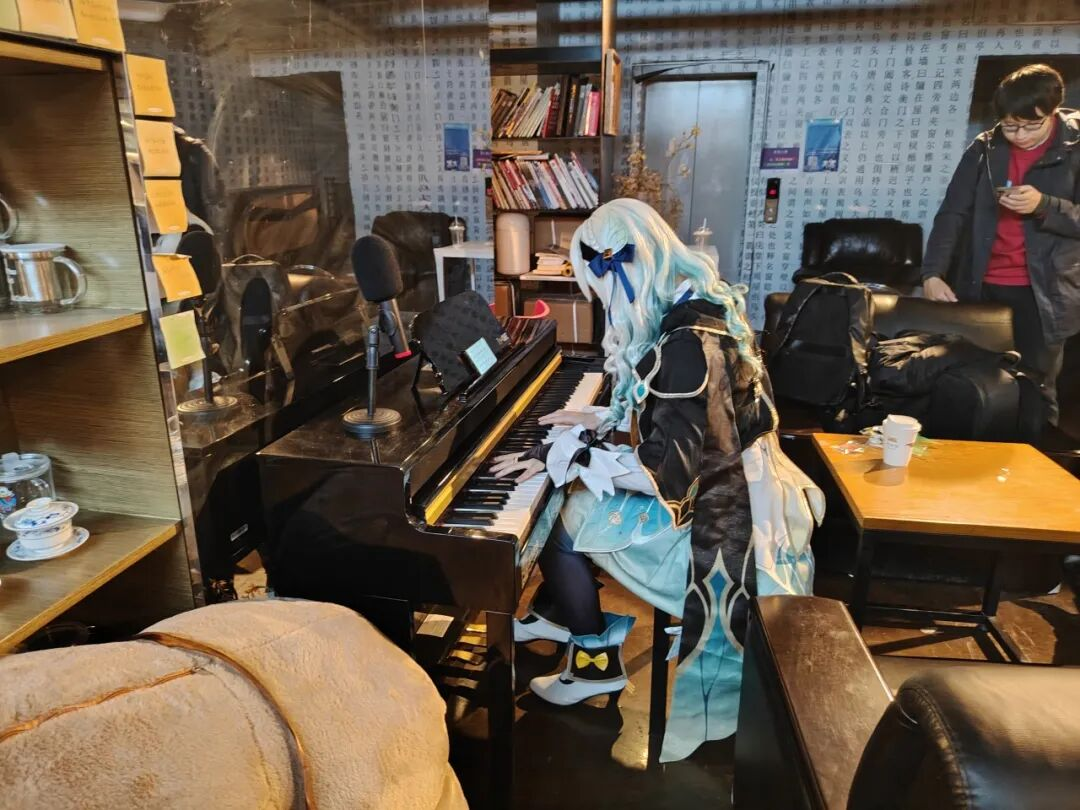
\includegraphics[width=0.9\linewidth]{咖啡厅4.jpg}}
		\vspace{-0.5em}
		\picbox{\small ~\ding{115} ~ 高雅的演奏家~}
		\normalsize
    \par
		\chind 动漫咖啡厅是每学期一度的,历史最悠久的次世代特色活动。\\
\chind 咖啡厅的咖啡师和服务生均由社员担任,不仅会提供各式点心和饮品特调,而且有紧张刺激的新番毒奶大会、剧场版动画连续放送,以及桌游、动画歌牌等游戏互动,还会不定期有茶绘现场看哦。当然还有必不可少的抽奖环节.jpg\\
\chind 这里同时也是cosplay的绝妙场所、外社联动的常见平台。\\
		\par
		\vspace{-2em}
		\raisebox{-\height}{
			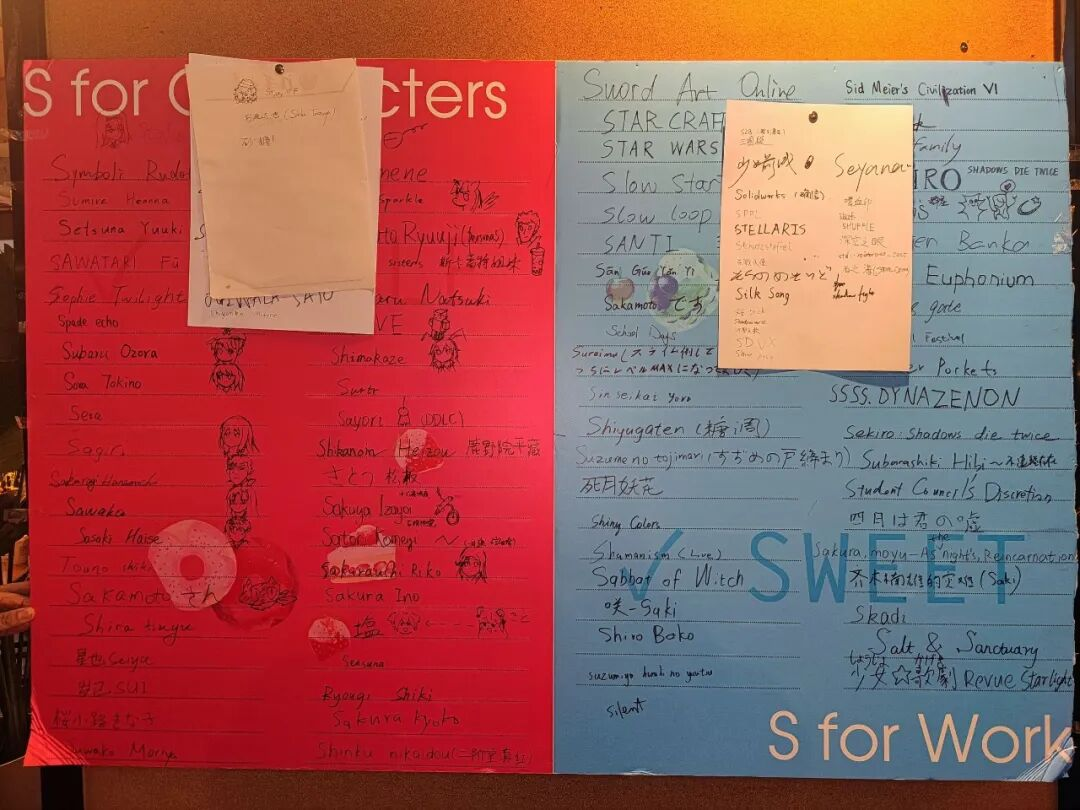
\includegraphics[width=0.8\linewidth]{咖啡厅5.jpg}}
		\vspace{-0.5em}
		\picbox{\small ~\ding{115} ~ S for what?~}

	\end{minipage}%
}
\begin{textblock*}{\paperwidth}(0mm, \dimexpr\paperheight-78.5mm\relax) % 距顶部 = 纸高 - 30mm
  \noindent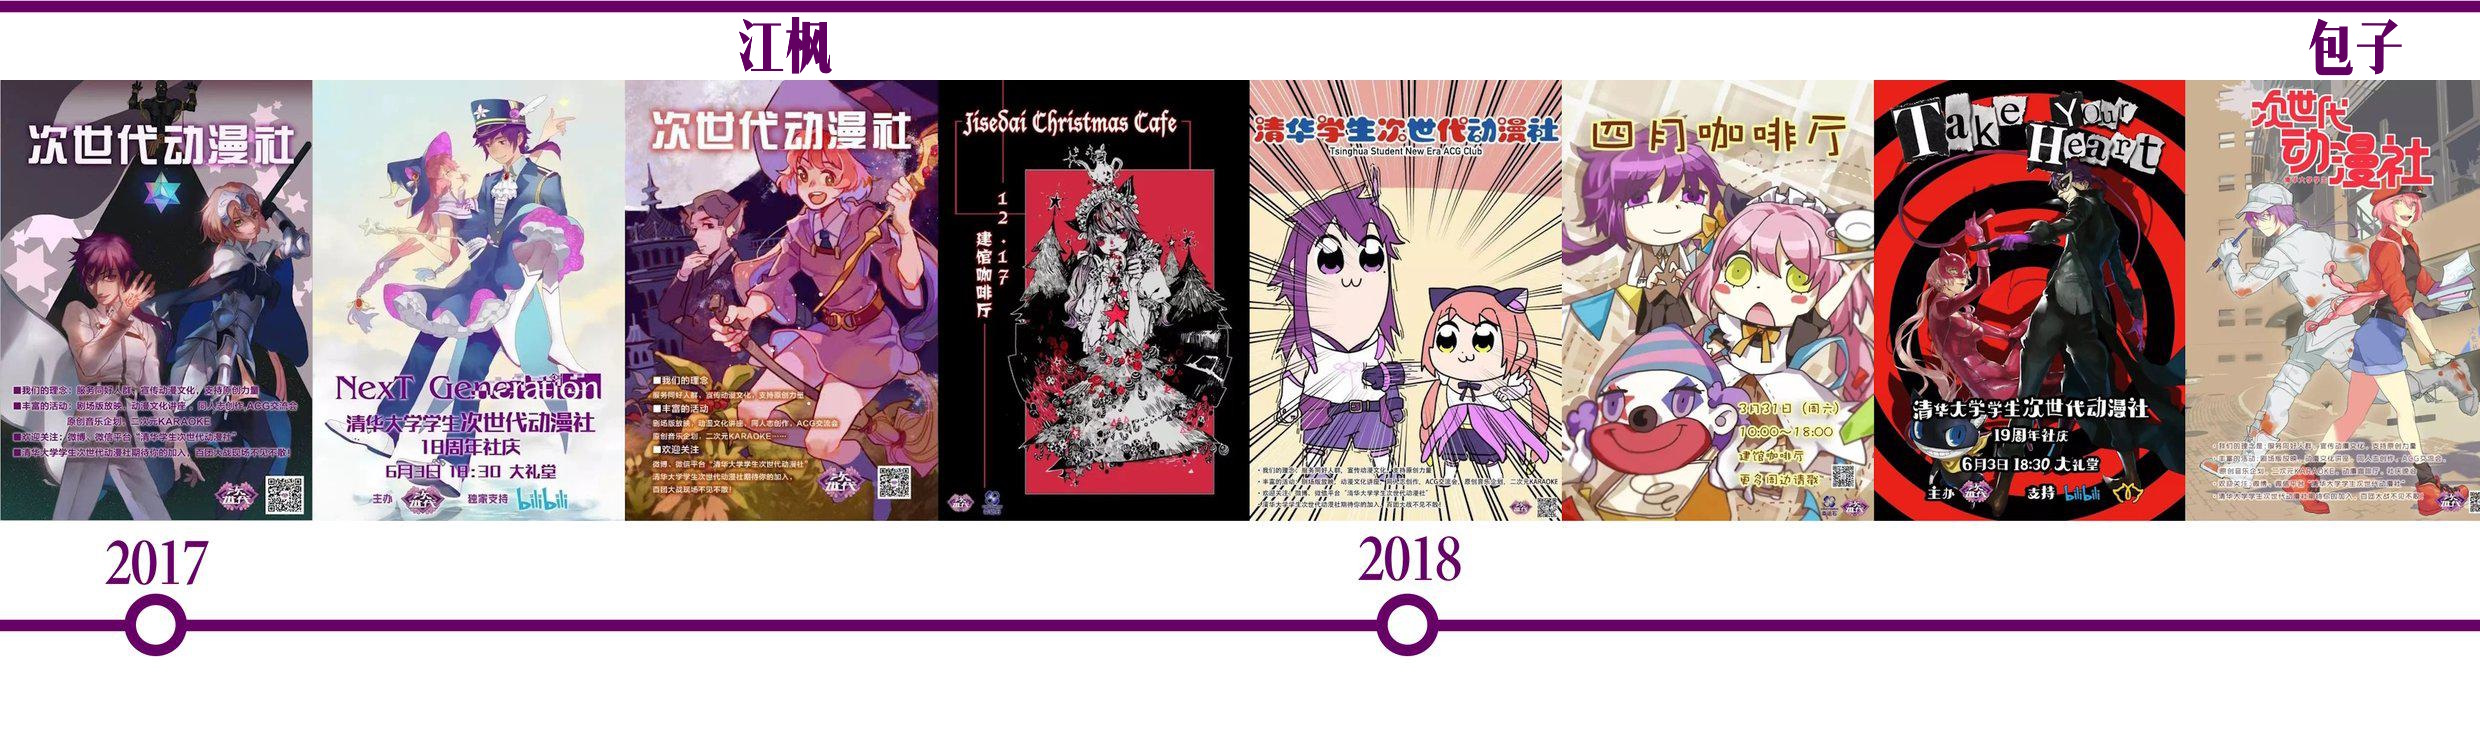
\includegraphics[width=\paperwidth]{tl2.jpg}
\end{textblock*}
\newpage
\fontsize{26pt}{28pt}\selectfont
\begin{center}
    \textbf{\textcolor{truepurple}{次世代社庆}}\\
\end{center}
\normalsize
\chind 一年一度,由各兴趣部门共同精心打造,\textbf{与学生节同等规格的大型ACGN主题晚会}。目前已经举办了13届!\sout{(大型网友面基现场)}\\
\chind 如果你对一份属于自己的二次元舞台有梦想,无论梦中的你是翩翩起舞的舞者还是激昂澎湃的乐手,是倾情演绎的演员还是引亢高歌的最强音,是聚光灯下的主持人还是幕后奉献的staff,所有的岗席与角色正虚位以待;\\
\chind 如果你只想坐在观众席欣赏表演,那么除了欣赏节目之外,也可以参与宅力大比拼的一站到底,抑或等待欧皇附体成为抽奖的幸运儿,当然无论如何都有三位看板的免费周边放送!\\
\chind 作为次世代最为盛大的年度活动,社庆为每一位心怀梦想的社友提供了施展才华的舞台。身为次世代社员的你怎能错过!\\
\vspace{1em}
\par
\adjustbox{valign=t}{
	\begin{minipage}[t]{0.45\textwidth}
		
		\raisebox{-\height}{
			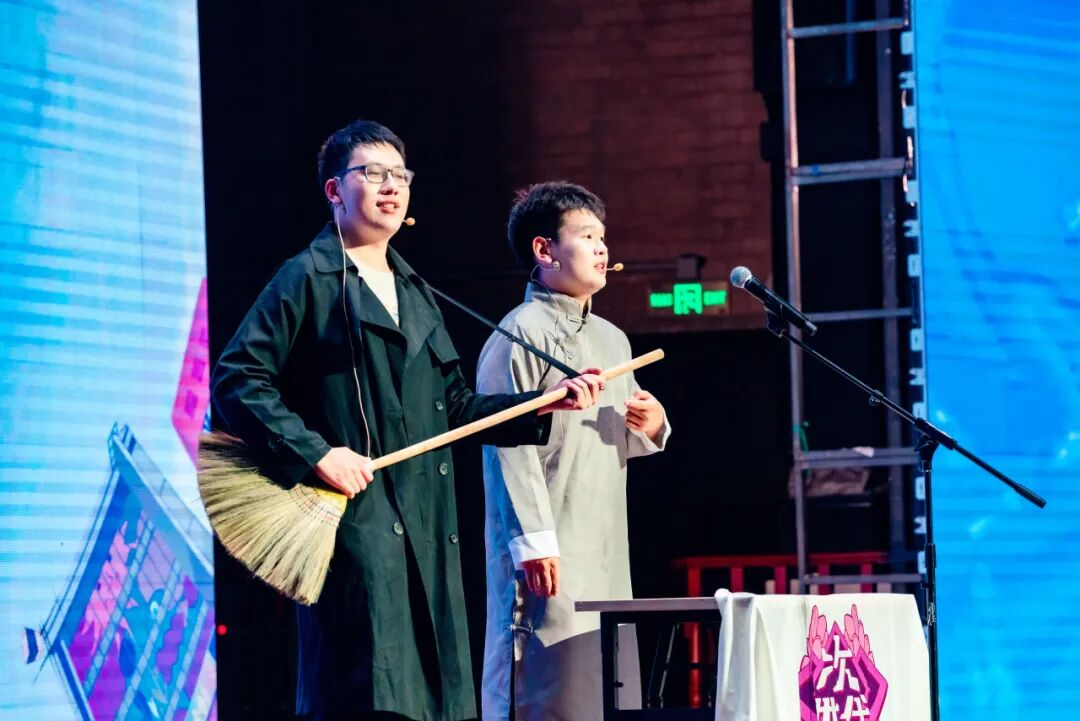
\includegraphics[width=0.9\linewidth]{社庆3.jpg}}
		\vspace{-0.5em}
		\picbox{\small \ding{115} 传世经典相声《我要玩乐队》}
  		\par
		\vspace{-0.5em}
		\raisebox{-\height}{
			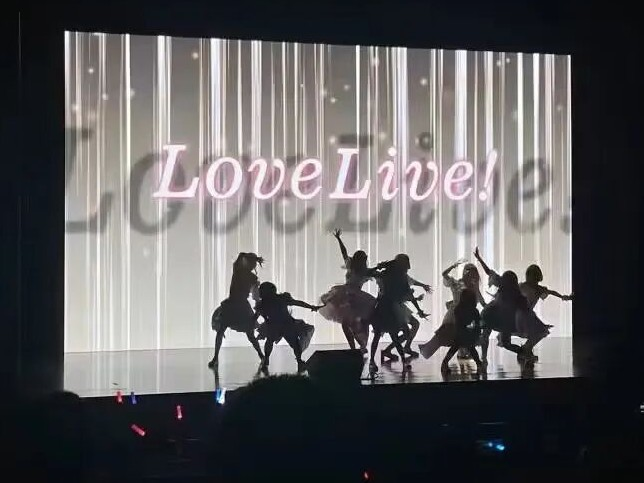
\includegraphics[width=0.9\linewidth]{社庆1.jpg}}
		\vspace{-0.5em}
		\picbox{\small ~\ding{115} ~ Lovelive!特别节目~}
	\end{minipage}}
\hfill
\vspace{1em}
\adjustbox{valign=t}{
	\begin{minipage}[t]{0.45\textwidth}
		\par
    
		\raisebox{-\height}{
			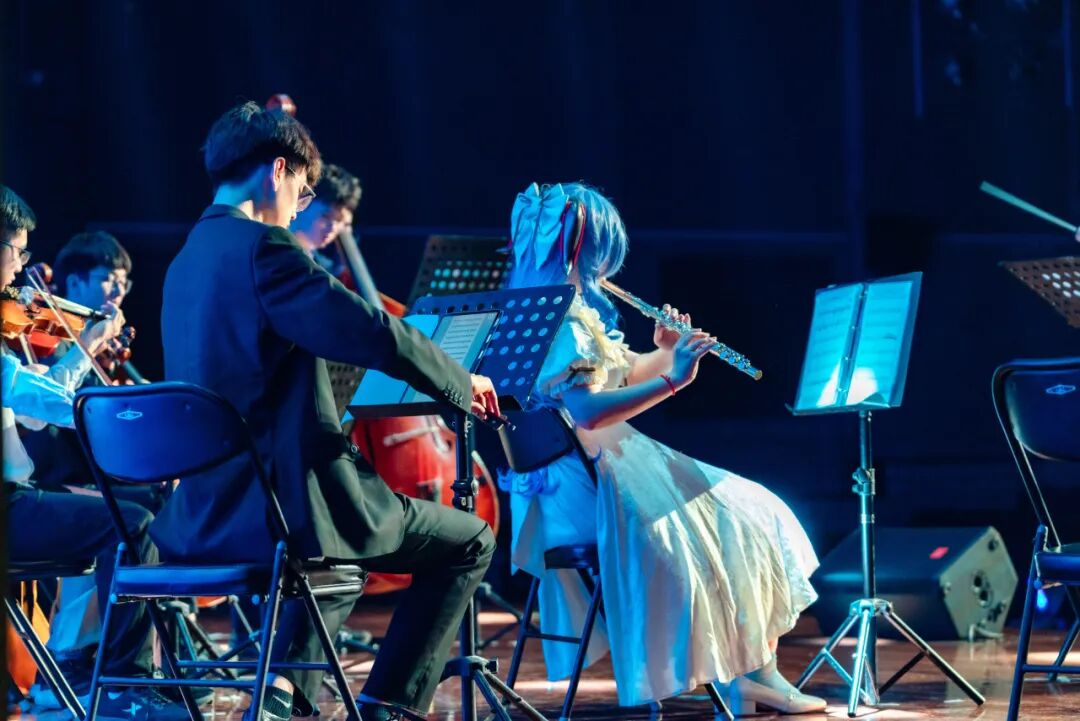
\includegraphics[width=0.9\linewidth]{社庆4.jpg}}
		\vspace{-0.5em}
		\picbox{\small ~\ding{115} ~ 室内乐节目~}
		\normalsize
    \par
		\vspace{0.5em}
		\raisebox{-\height}{
			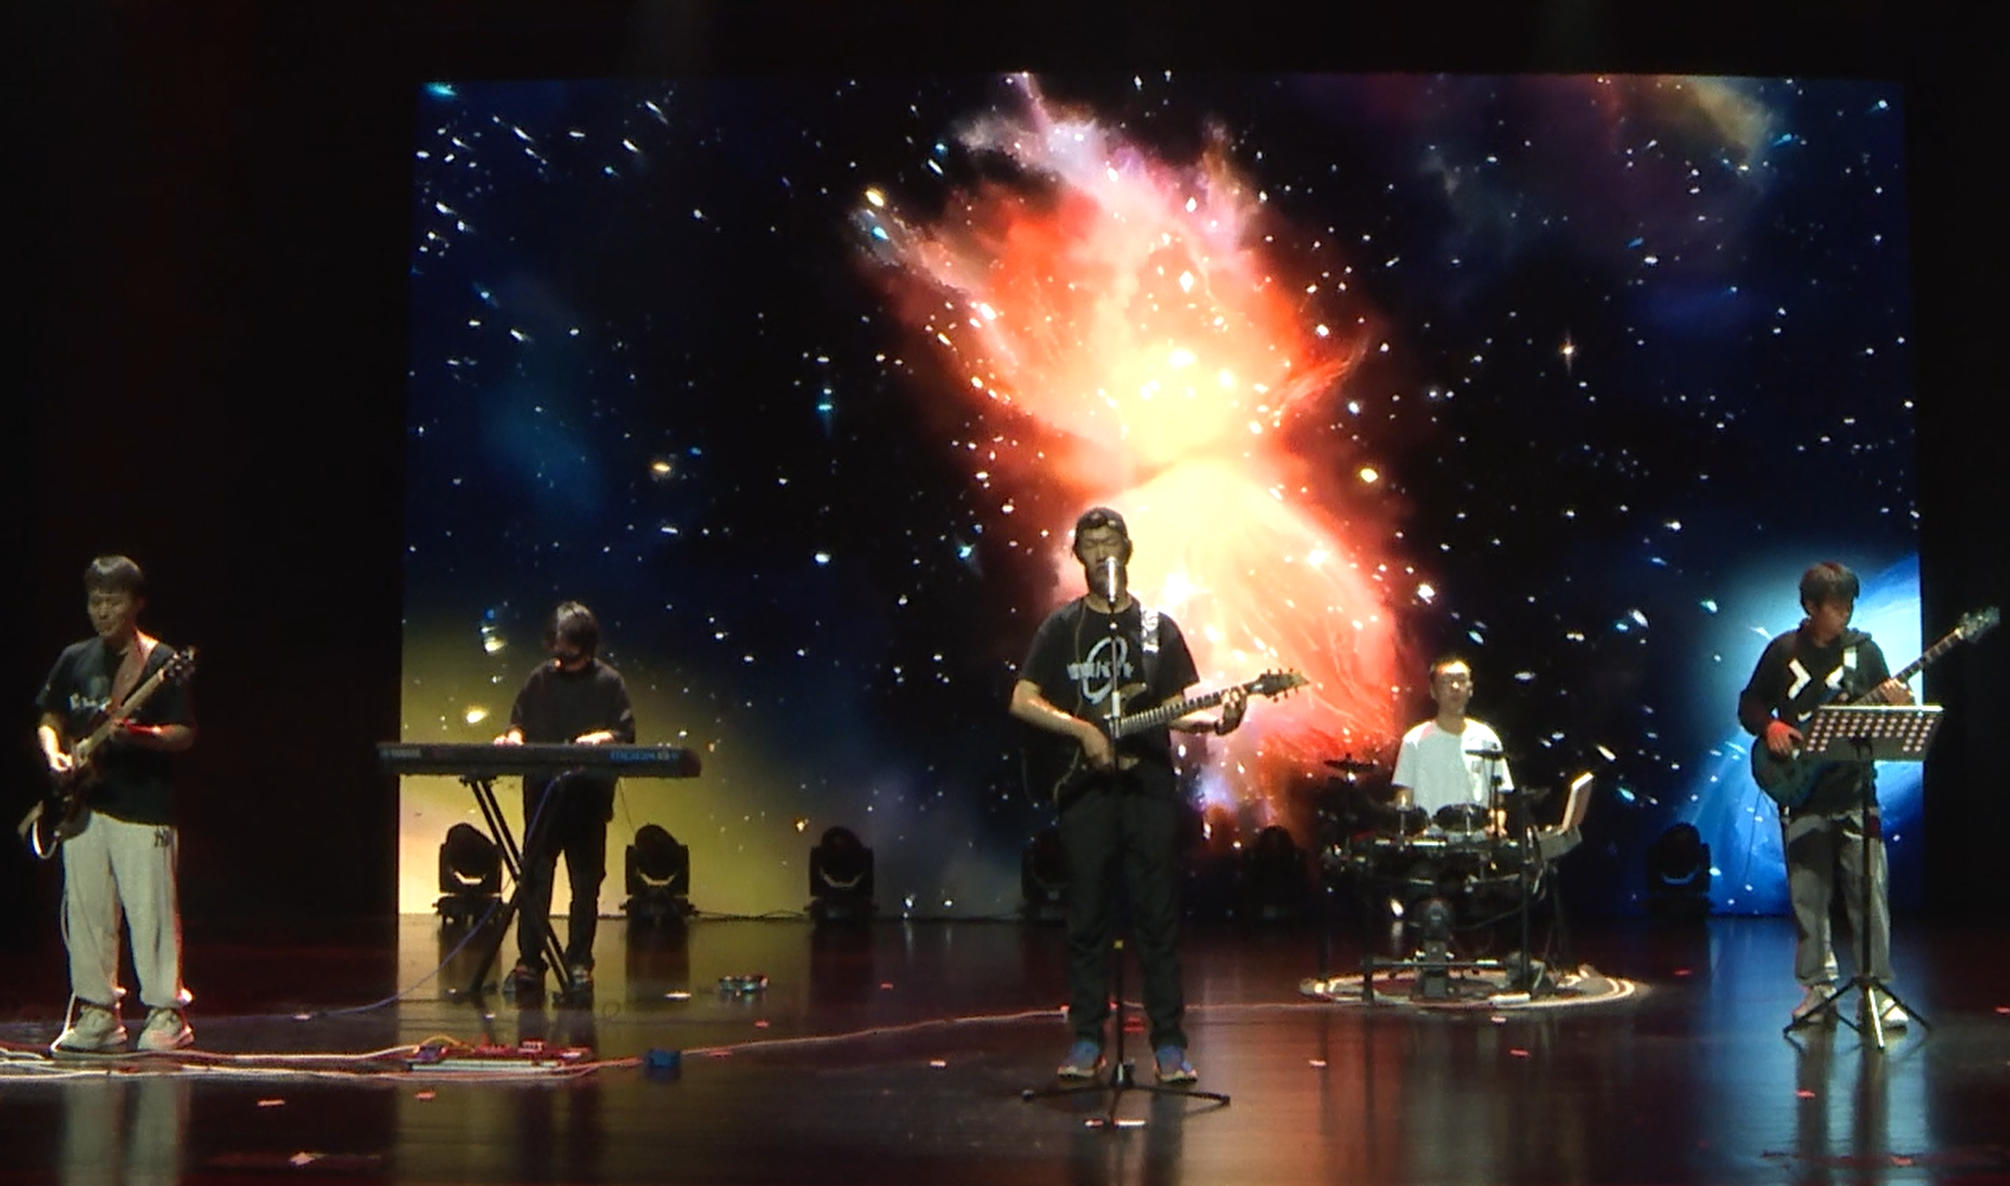
\includegraphics[width=0.9\linewidth]{社庆10.jpg}}
		\vspace{-0.5em}
		\picbox{\small ~\ding{115} ~ 乐队开场《再飞行》~}

	\end{minipage}%
}
\begin{textblock*}{\paperwidth}(0mm, \dimexpr\paperheight-78.5mm\relax) % 距顶部 = 纸高 - 30mm
  \noindent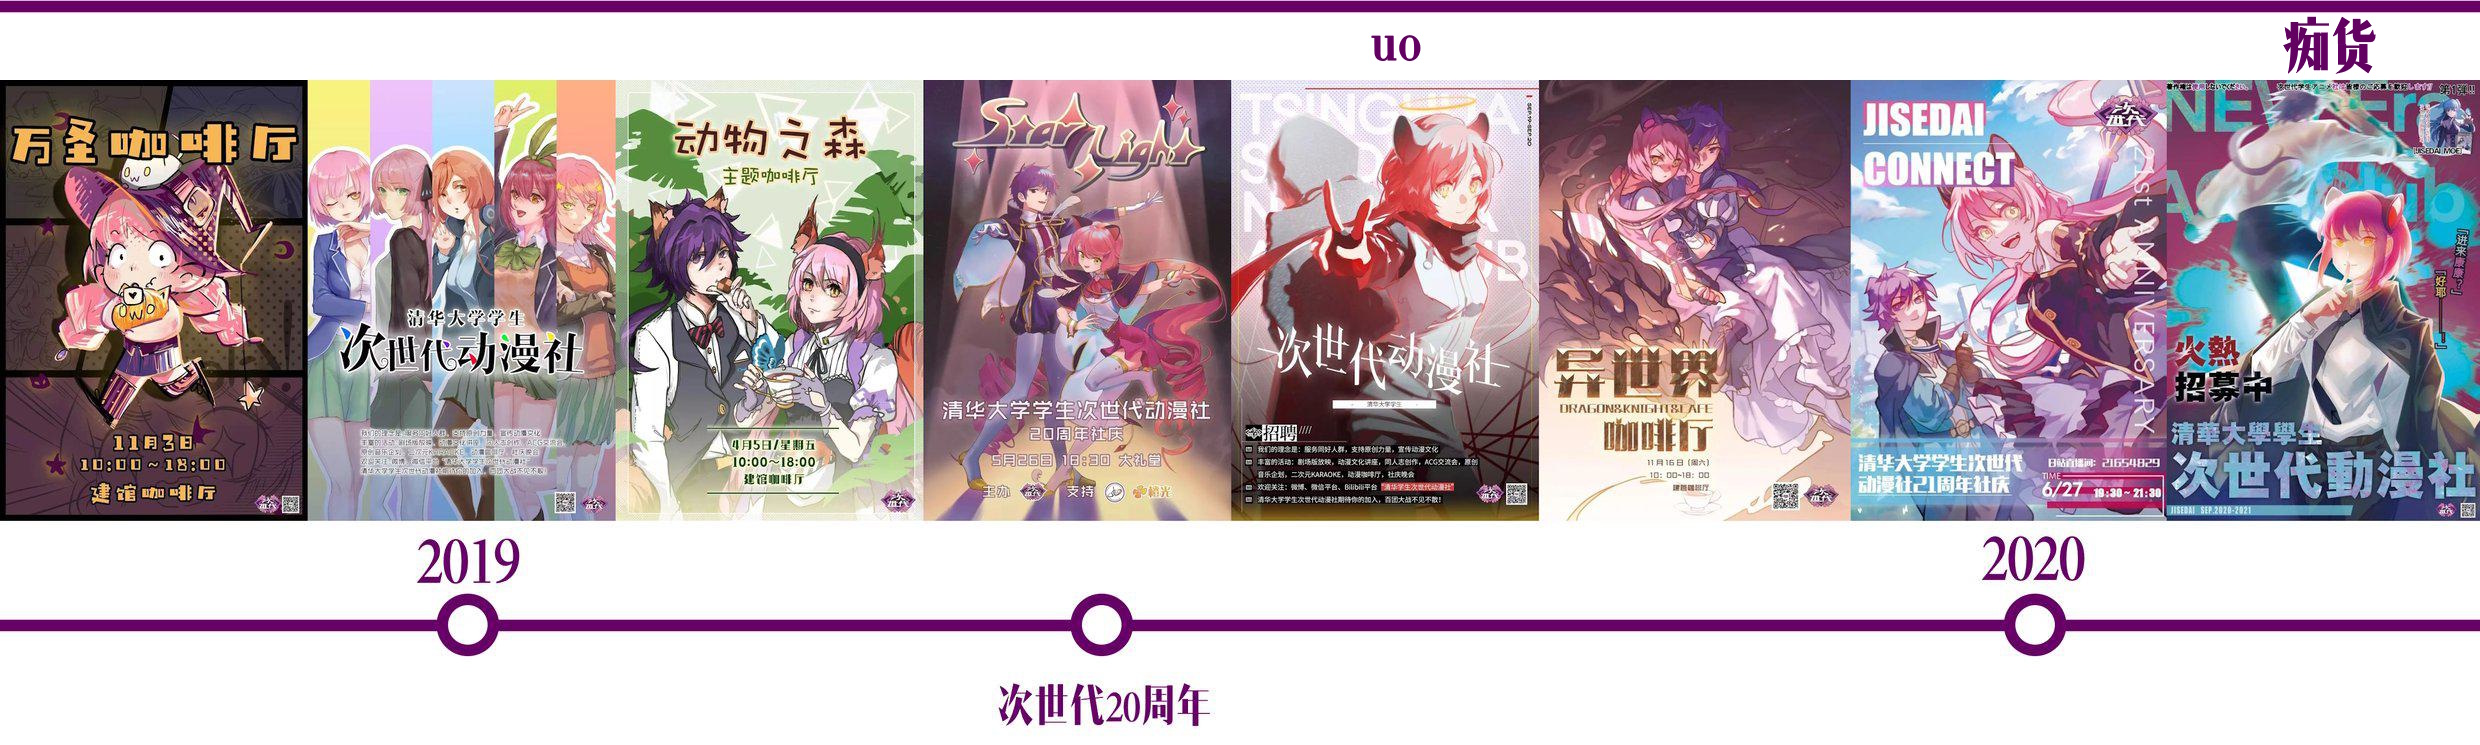
\includegraphics[width=\paperwidth]{tl3.jpg}
\end{textblock*}



\newpage
\par
\adjustbox{valign=t}{
	\begin{minipage}[t]{0.45\textwidth}
		
		\raisebox{-\height}{
			\includegraphics[width=0.9\linewidth]{社庆5.jpg}}
		\vspace{-0.5em}
		\picbox{\small \ding{115} 舞台剧《苹果默示录》}
  		\par
		\vspace{-0.5em}
		\raisebox{-\height}{
			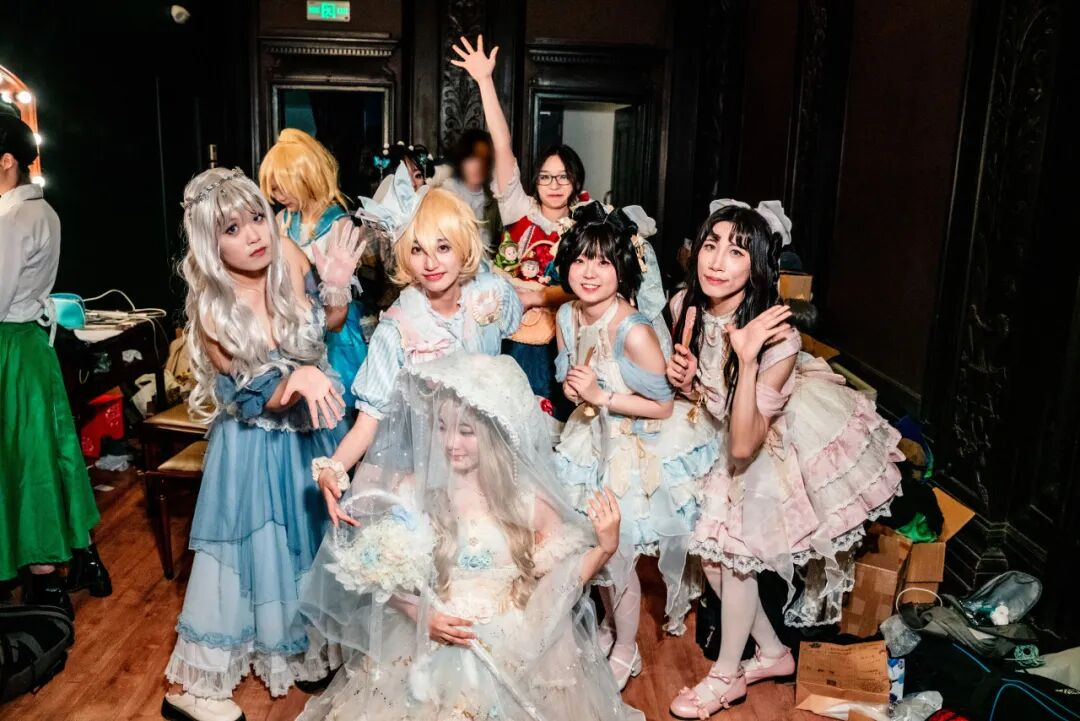
\includegraphics[width=0.9\linewidth]{社庆8.jpg}}
		\vspace{-0.5em}
		\picbox{\small ~\ding{115} ~ 在化妆间~}
	\end{minipage}}
\hfill
\vspace{1em}
\adjustbox{valign=t}{
	\begin{minipage}[t]{0.45\textwidth}
		\par
    
		\raisebox{-\height}{
			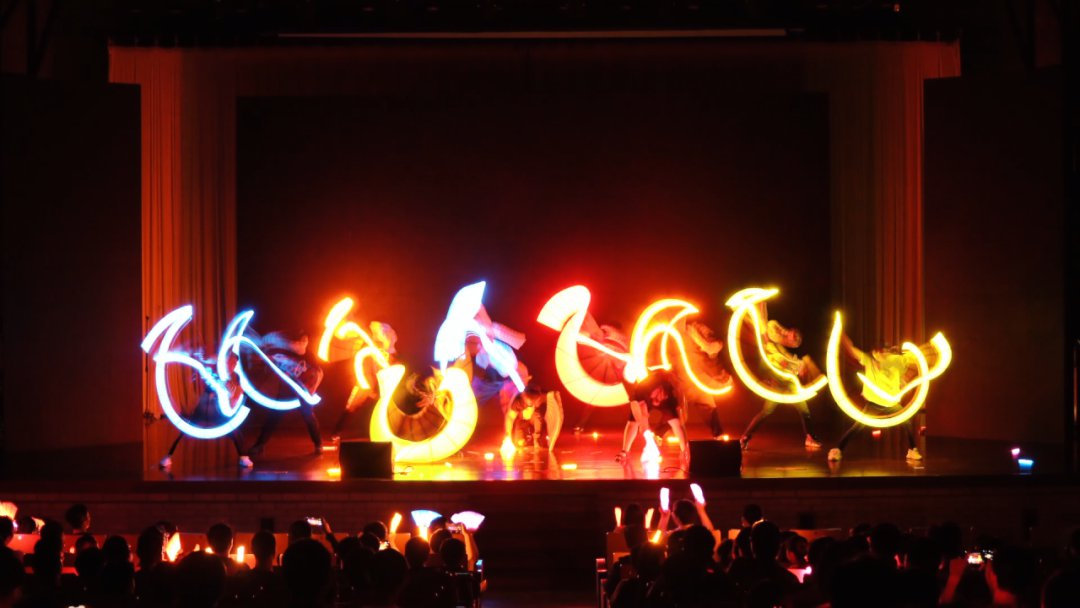
\includegraphics[width=0.9\linewidth]{社庆6.jpg}}
		\vspace{-0.5em}
		\picbox{\small ~\ding{115} ~ WOTA艺节目~}
		\normalsize
    \par
		\vspace{1.5em}
		\raisebox{-\height}{
			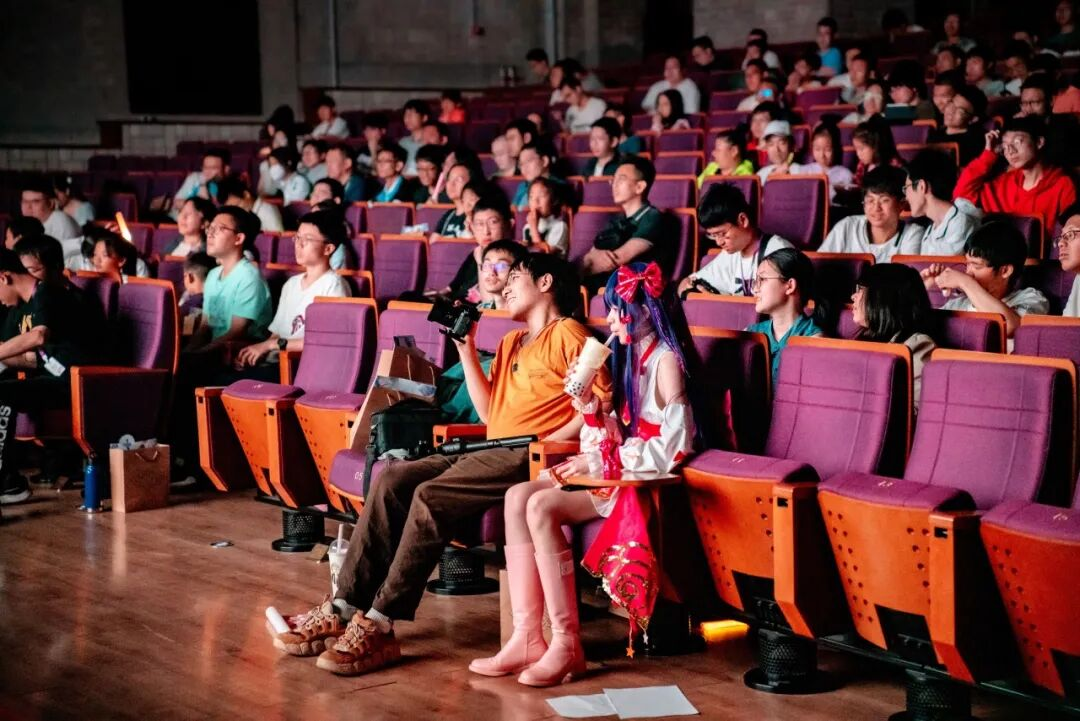
\includegraphics[width=0.9\linewidth]{社庆9.jpg}}
		\vspace{-0.5em}
		\picbox{\small ~\ding{115} ~ 溢出舞台的喜悦~}

	\end{minipage}%
}
\begin{center}
		\raisebox{-\height}{
			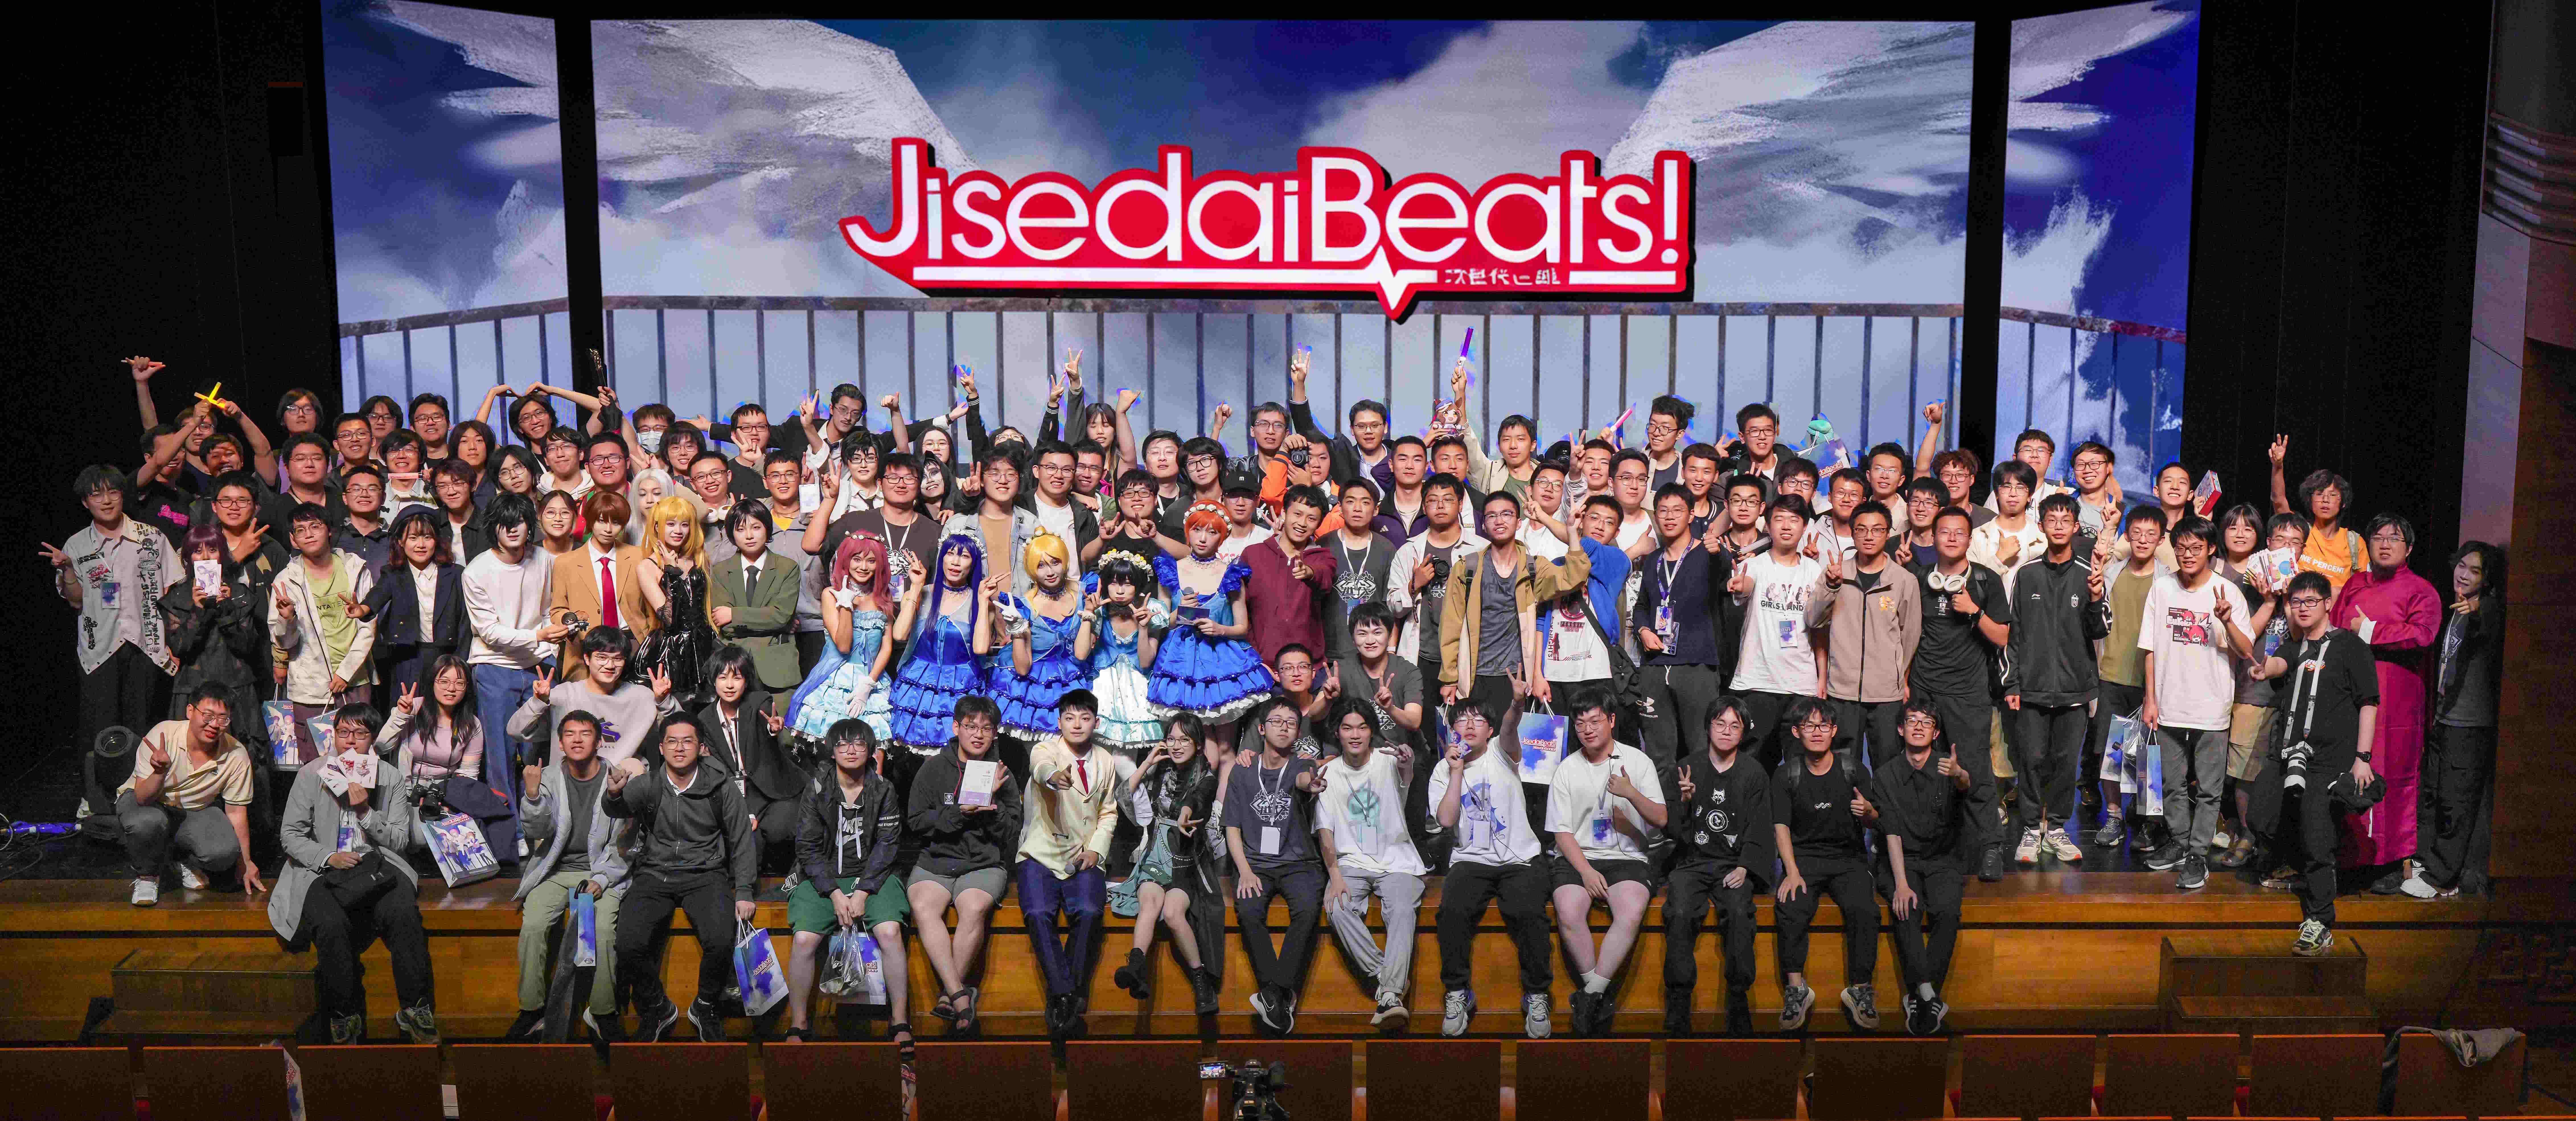
\includegraphics[width=0.9\linewidth]{社庆7.jpeg}}
		\vspace{-0.5em}
		\picbox{\small ~\ding{115} ~ 2025社庆~JisedaiBeats~大合照~}
\end{center}
\begin{textblock*}{\paperwidth}(0mm, \dimexpr\paperheight-78.5mm\relax) % 距顶部 = 纸高 - 30mm
  \noindent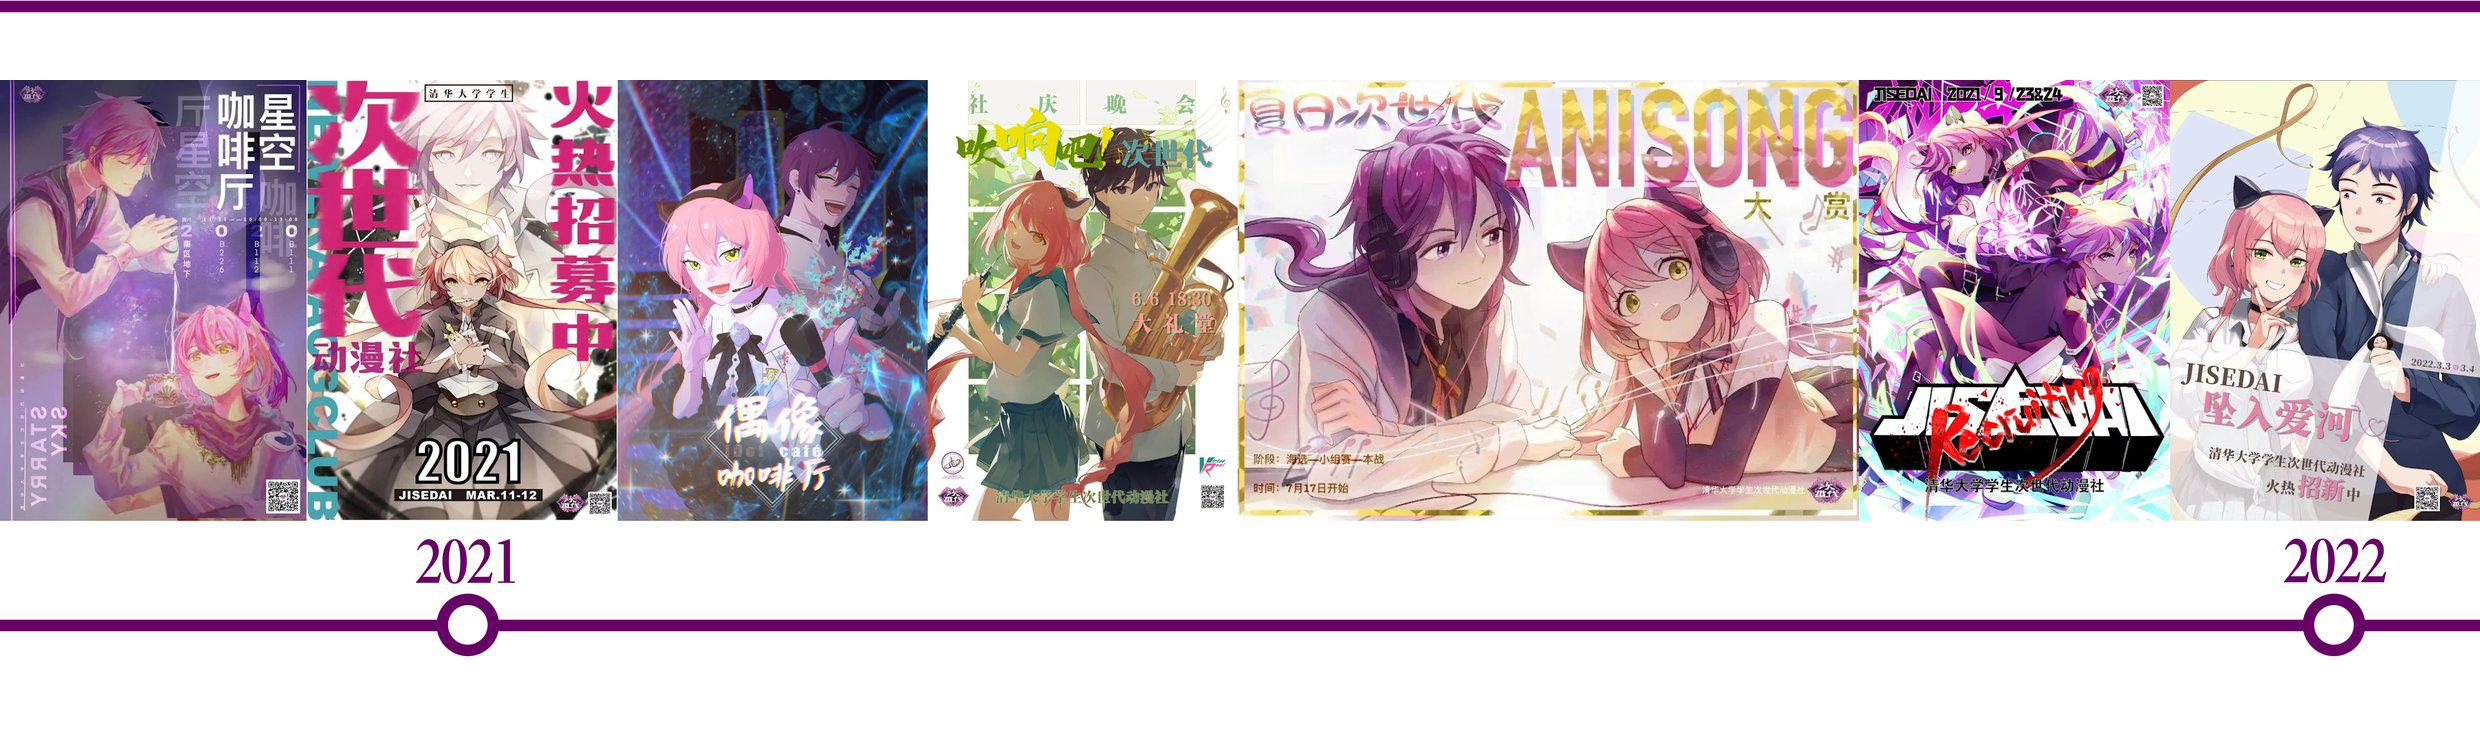
\includegraphics[width=\paperwidth]{tl4.jpg}
\end{textblock*}



\newpage
\fontsize{23pt}{24pt}\selectfont
\begin{center}
    \textbf{\textcolor{truepurple}{实验剧场乐队live}}\\
\end{center}
\vspace{-1em}
\adjustbox{valign=t}{
	\begin{minipage}[t]{0.45\textwidth}
		\vspace{0.5em}
		\raisebox{-\height}{
			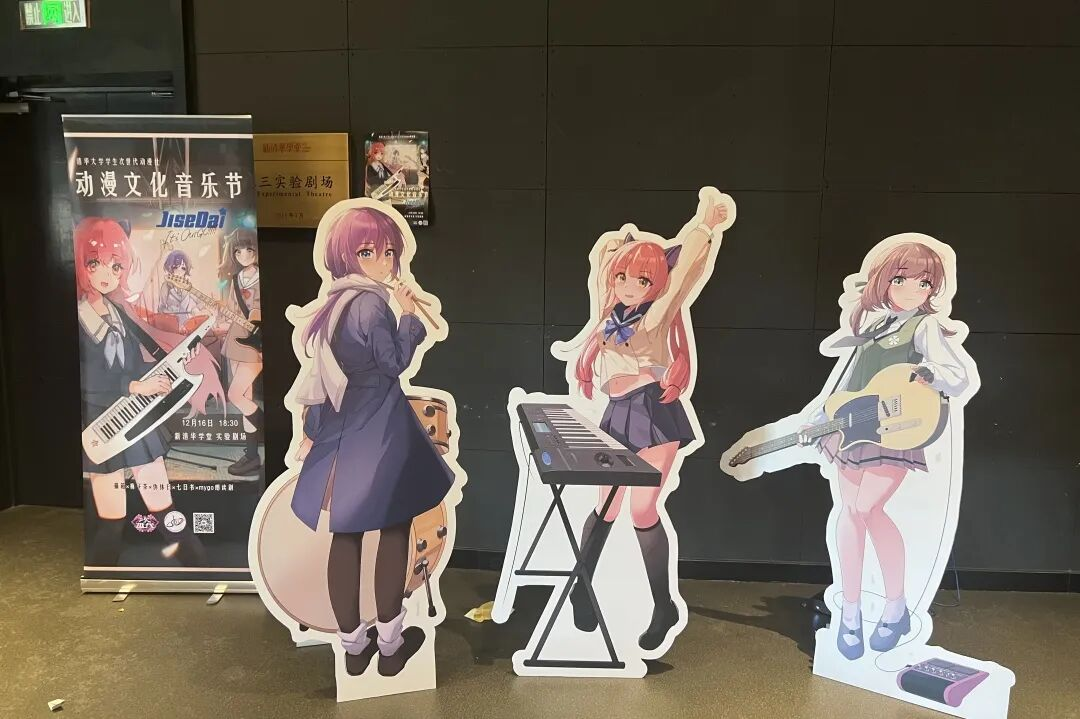
\includegraphics[width=\linewidth]{乐队4.jpg}}
    \par
		\vspace{0.5em}
		\raisebox{-\height}{
			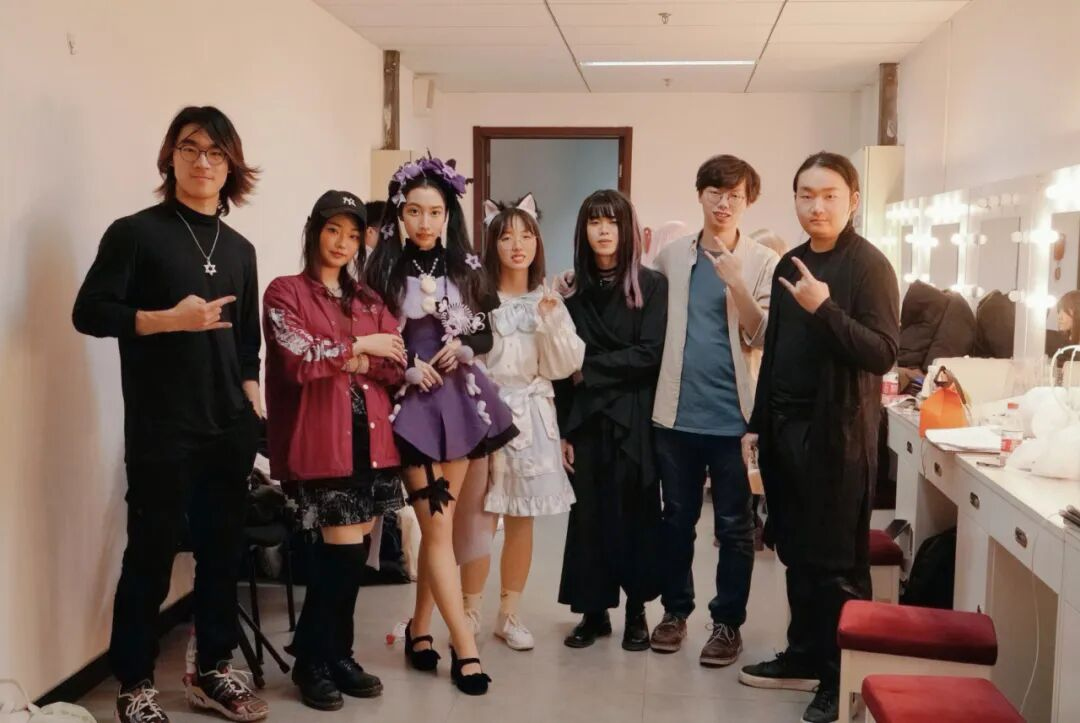
\includegraphics[width=\linewidth]{乐队5.jpg}}

		\normalsize
    \par
    \vspace{0.2em}
		\chind 作为乐队部的招牌项目,每学期一度、于新清华学堂实验剧场举行的乐队live都是一场乐队演出的狂欢。在这里,请你见证量大管饱的乐队表演:人声与演奏,拍动与旋律,演绎与原创……从ACGN到独立摇滚,从jpop到国漫经典,我们的歌单也构成着自我表达的电波。\\
    \chind 一首首曲子的呈现是各队队员一次次练习的结晶。希望我们的努力,足以回应大家为我们付出的每一张门票、每一秒时光、每一声应援。如果愿意的话,我们也欢迎台下的每一个你成为站到台上的一员。\\

	\end{minipage}}
\hfill
\adjustbox{valign=t}{
	\begin{minipage}[t]{0.45\textwidth}
    \vspace{0.4em}
		\raisebox{-\height}{
			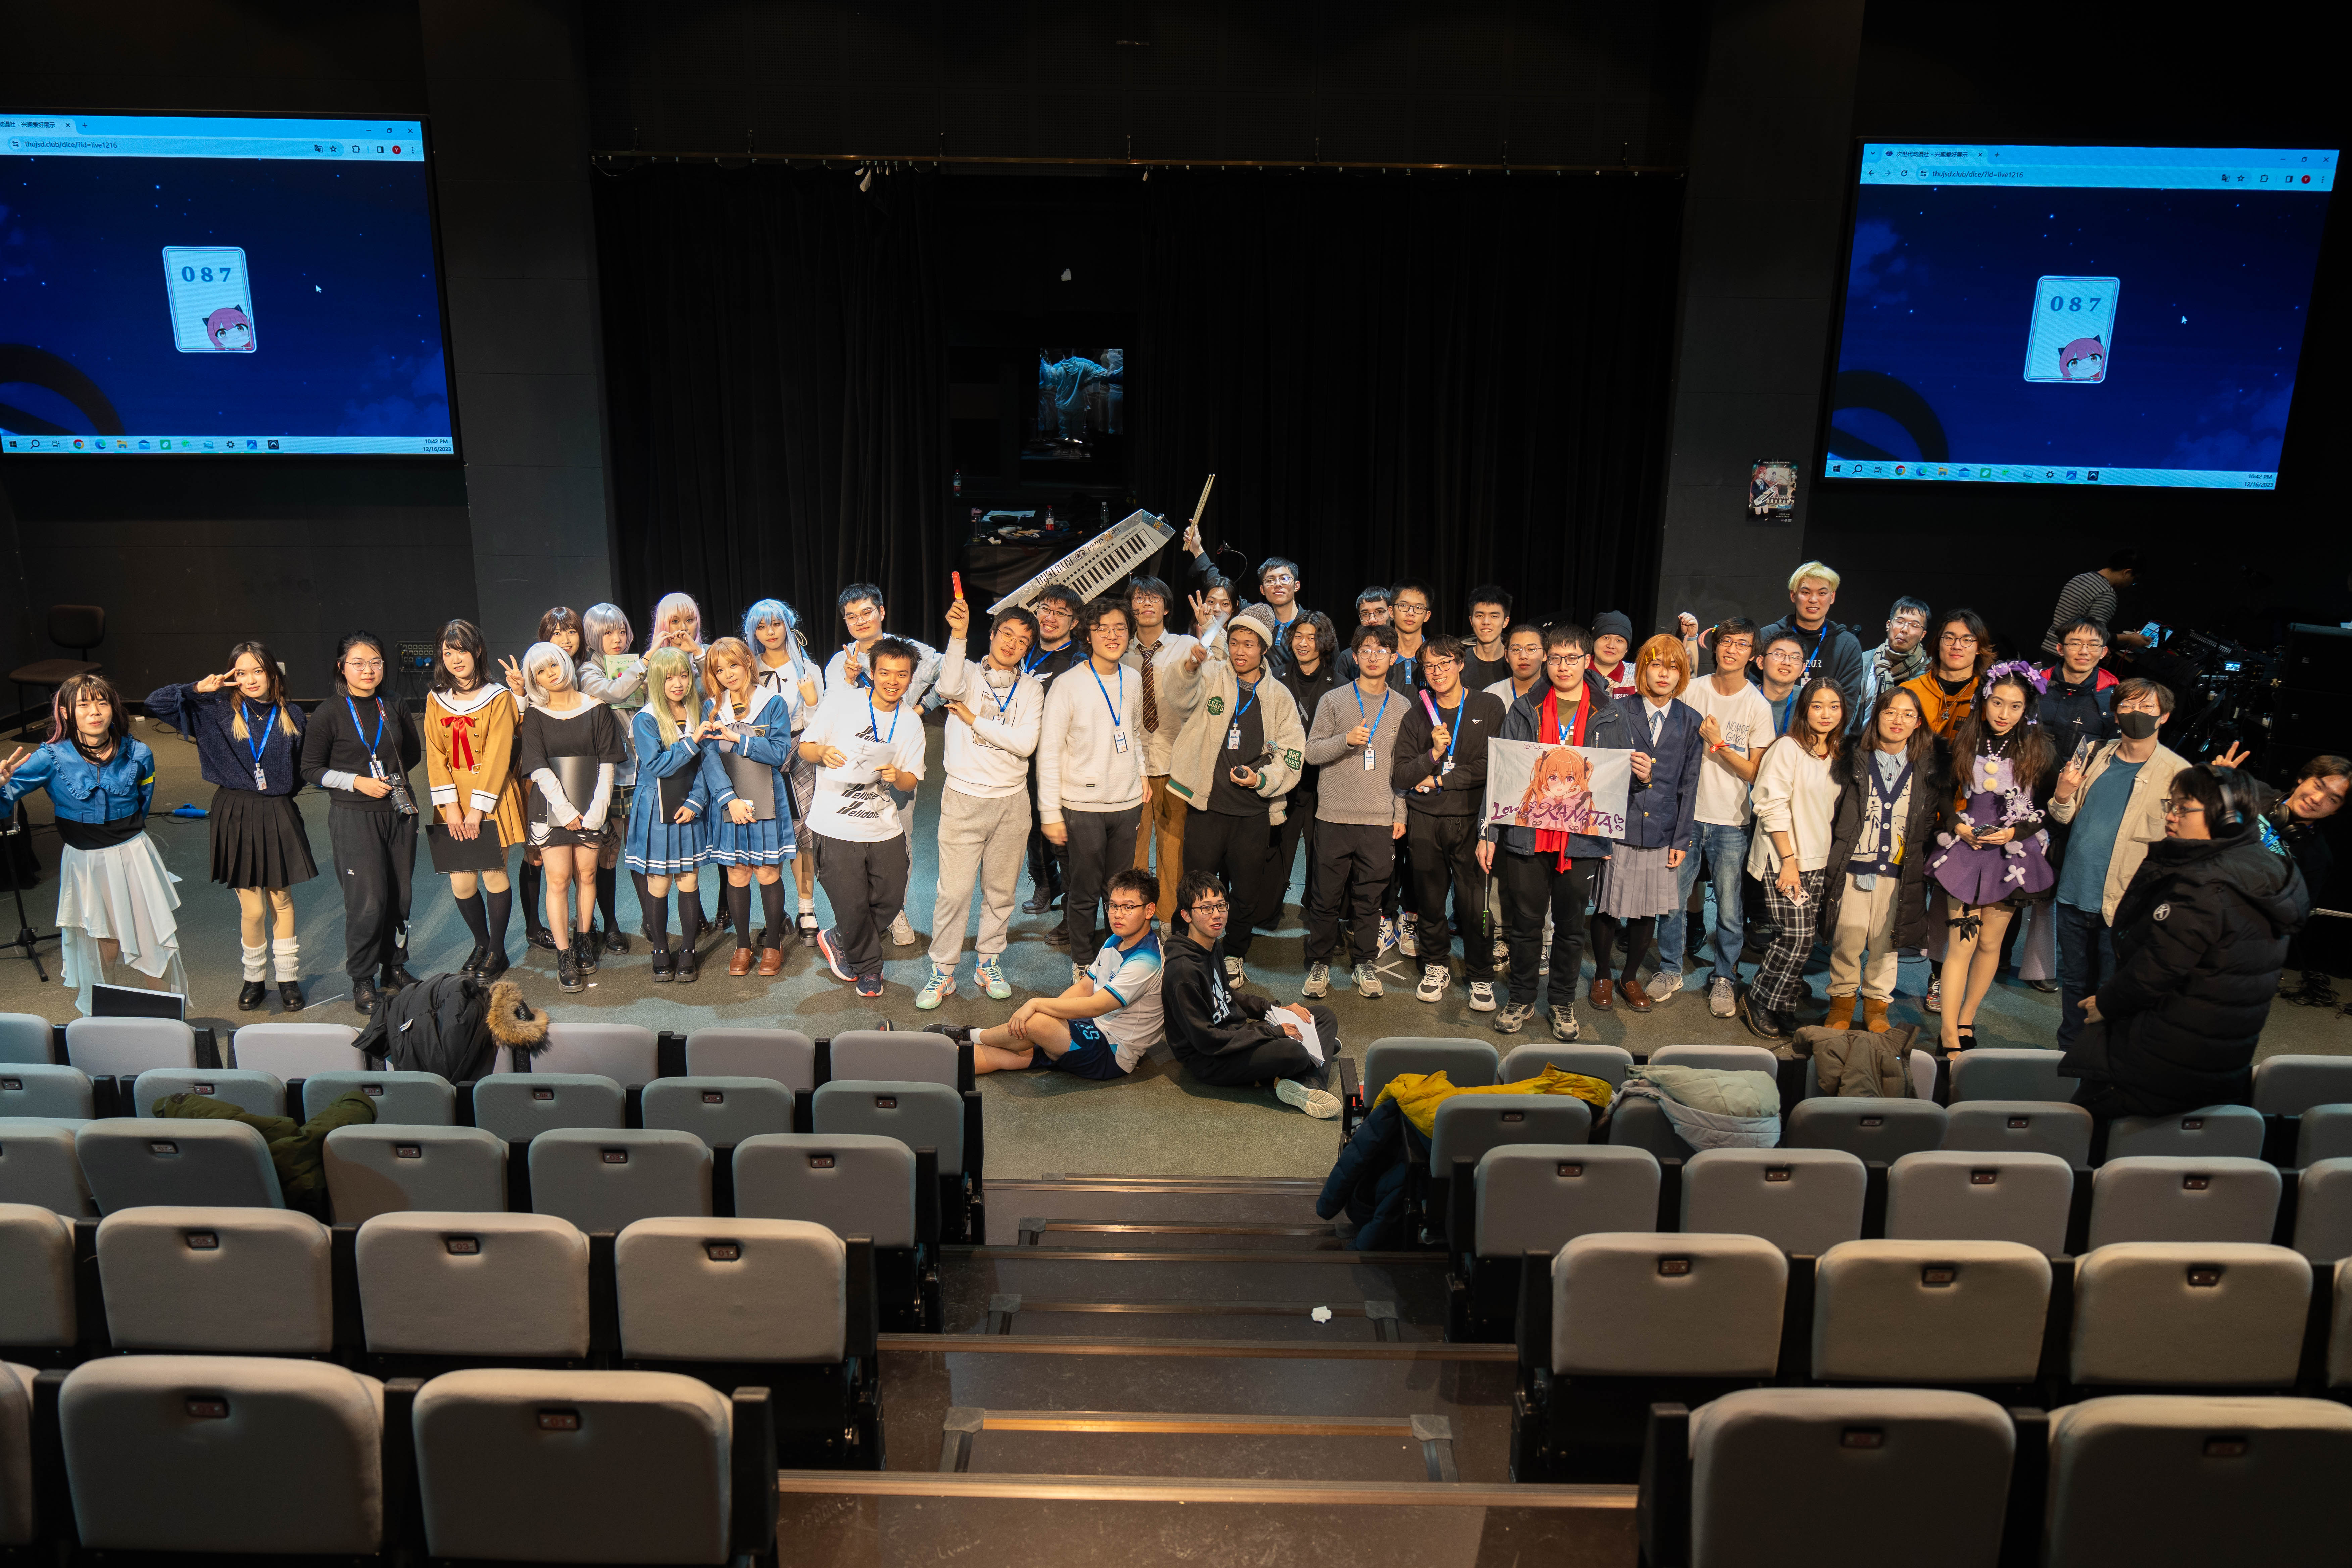
\includegraphics[width=\linewidth]{乐队1.jpg}}
		\par
		\vspace{0.5em}
		\raisebox{-\height}{
			\includegraphics[width=\linewidth]{乐队3.jpg}}
		\par
		\vspace{0.5em}
		\raisebox{-\height}{
			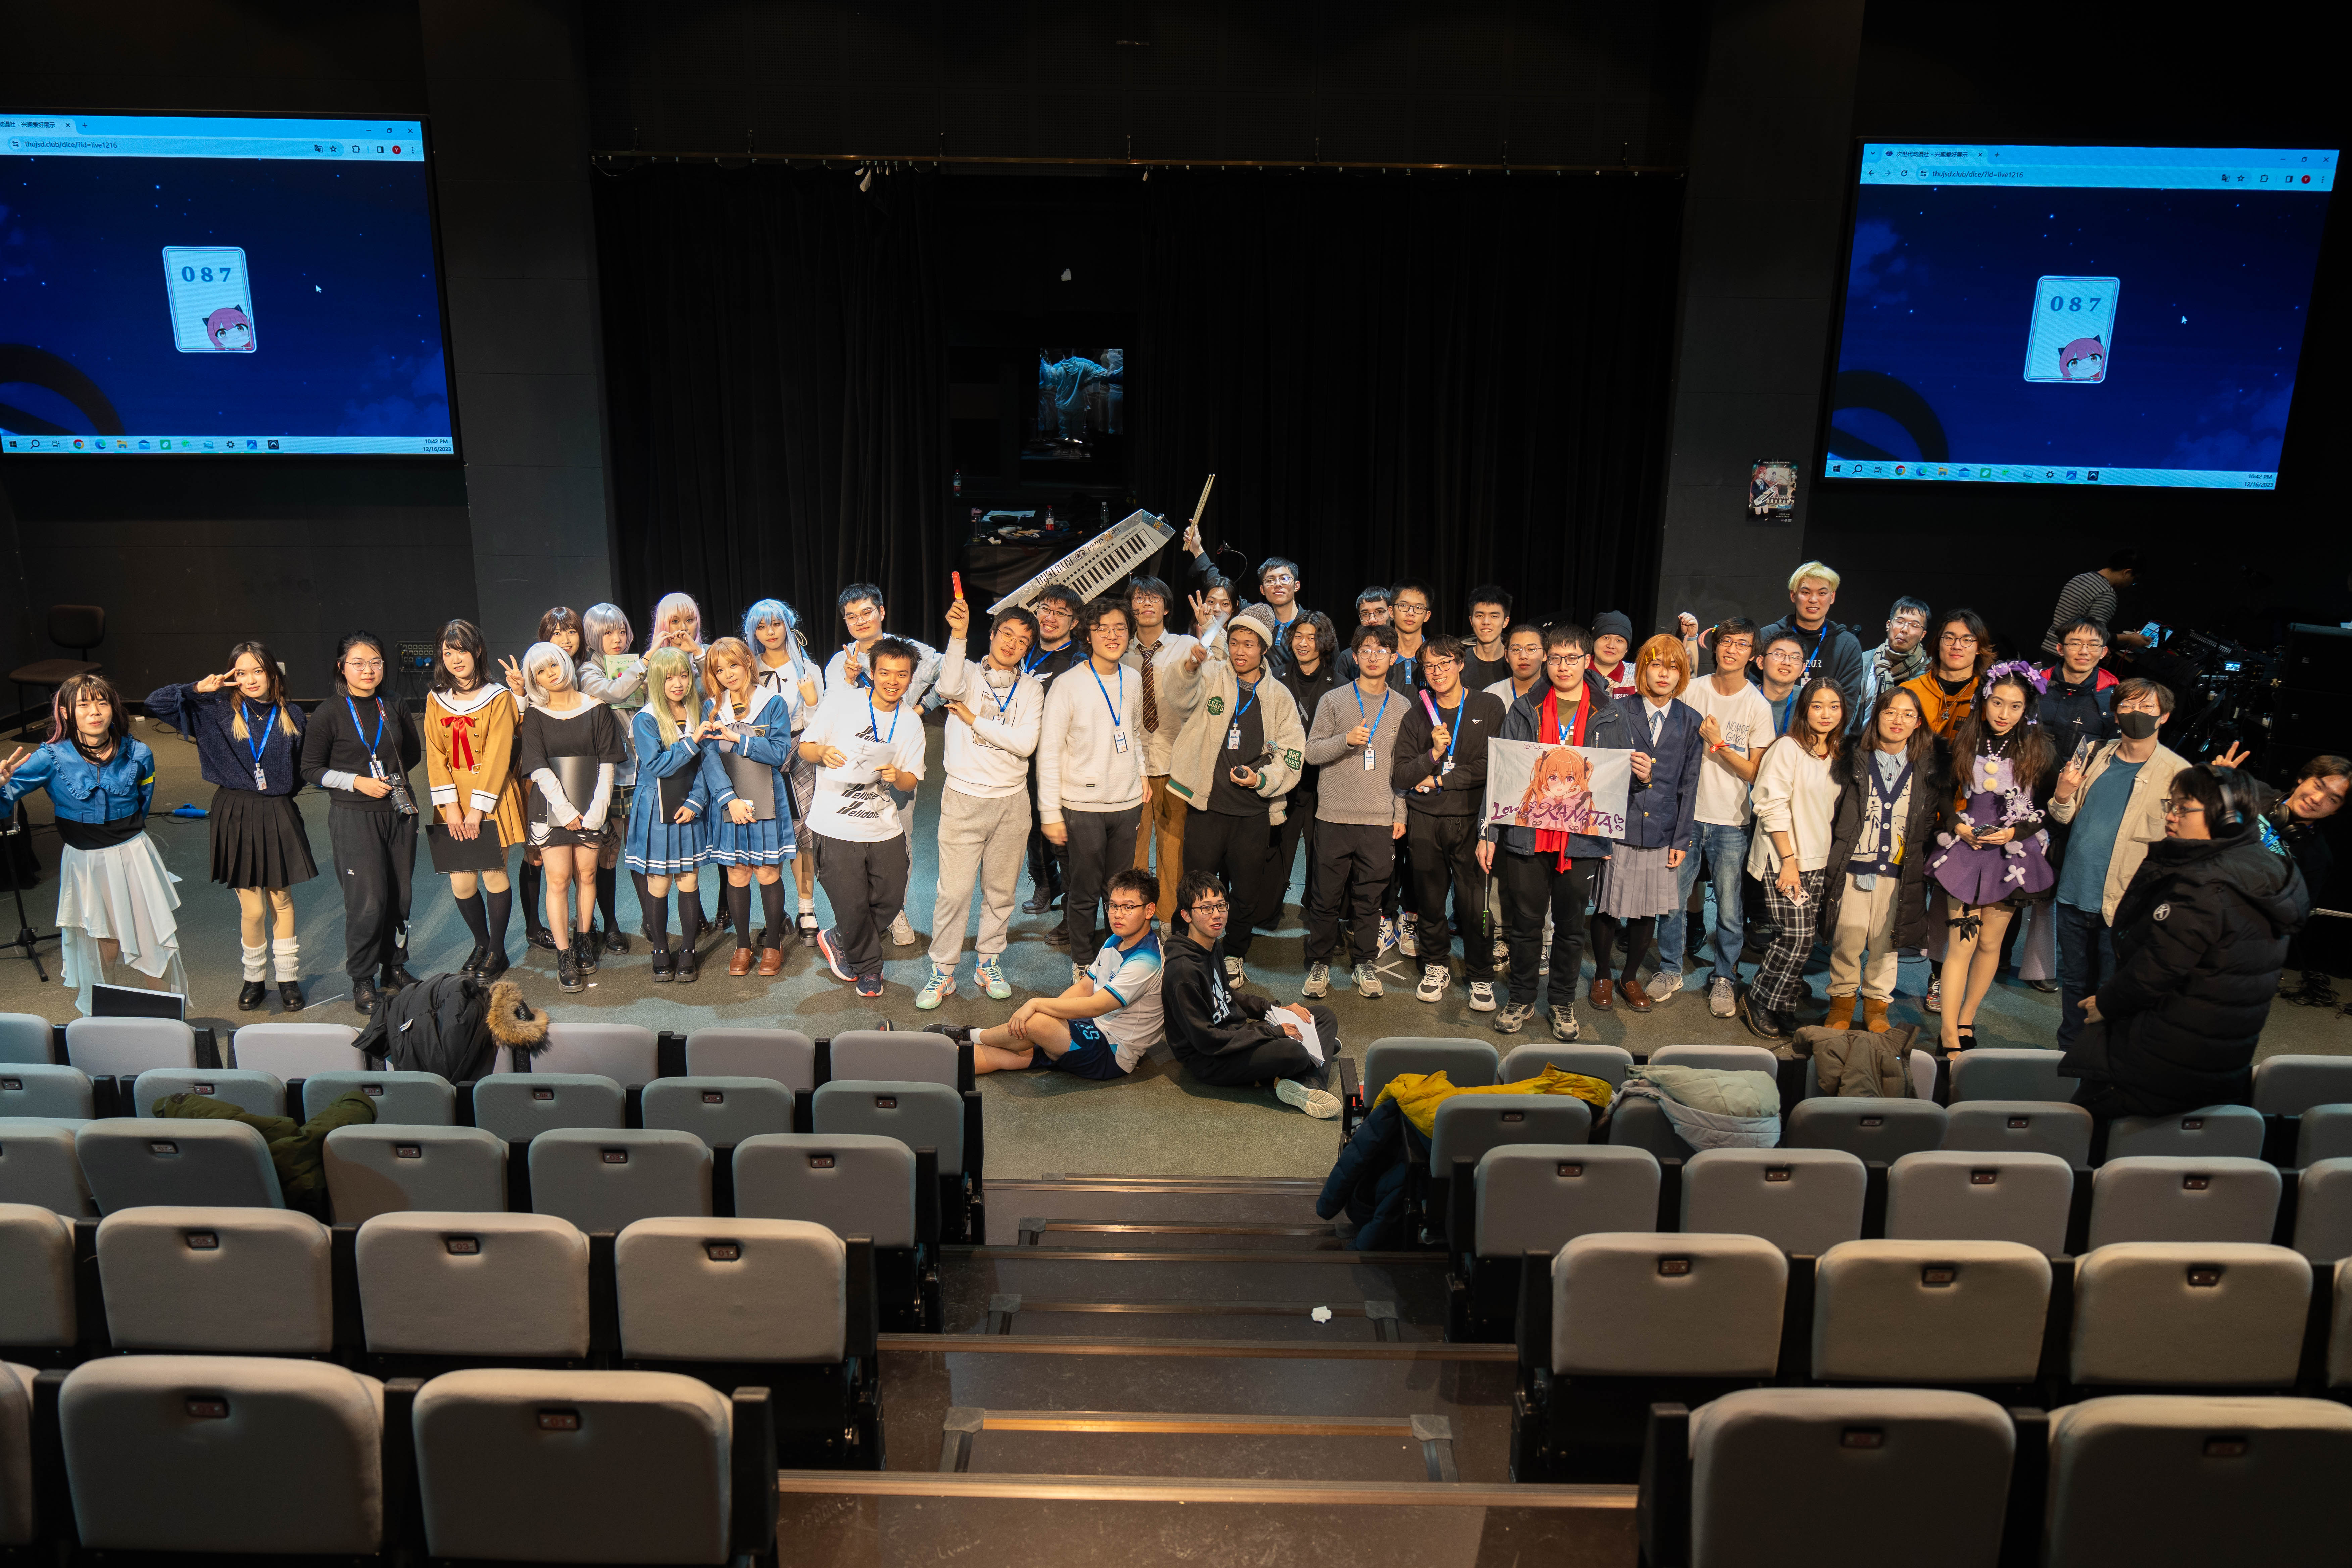
\includegraphics[width=\linewidth]{乐队2.jpg}}

	\end{minipage}%
}
\begin{textblock*}{\paperwidth}(0mm, \dimexpr\paperheight-78.5mm\relax) % 距顶部 = 纸高 - 30mm
  \noindent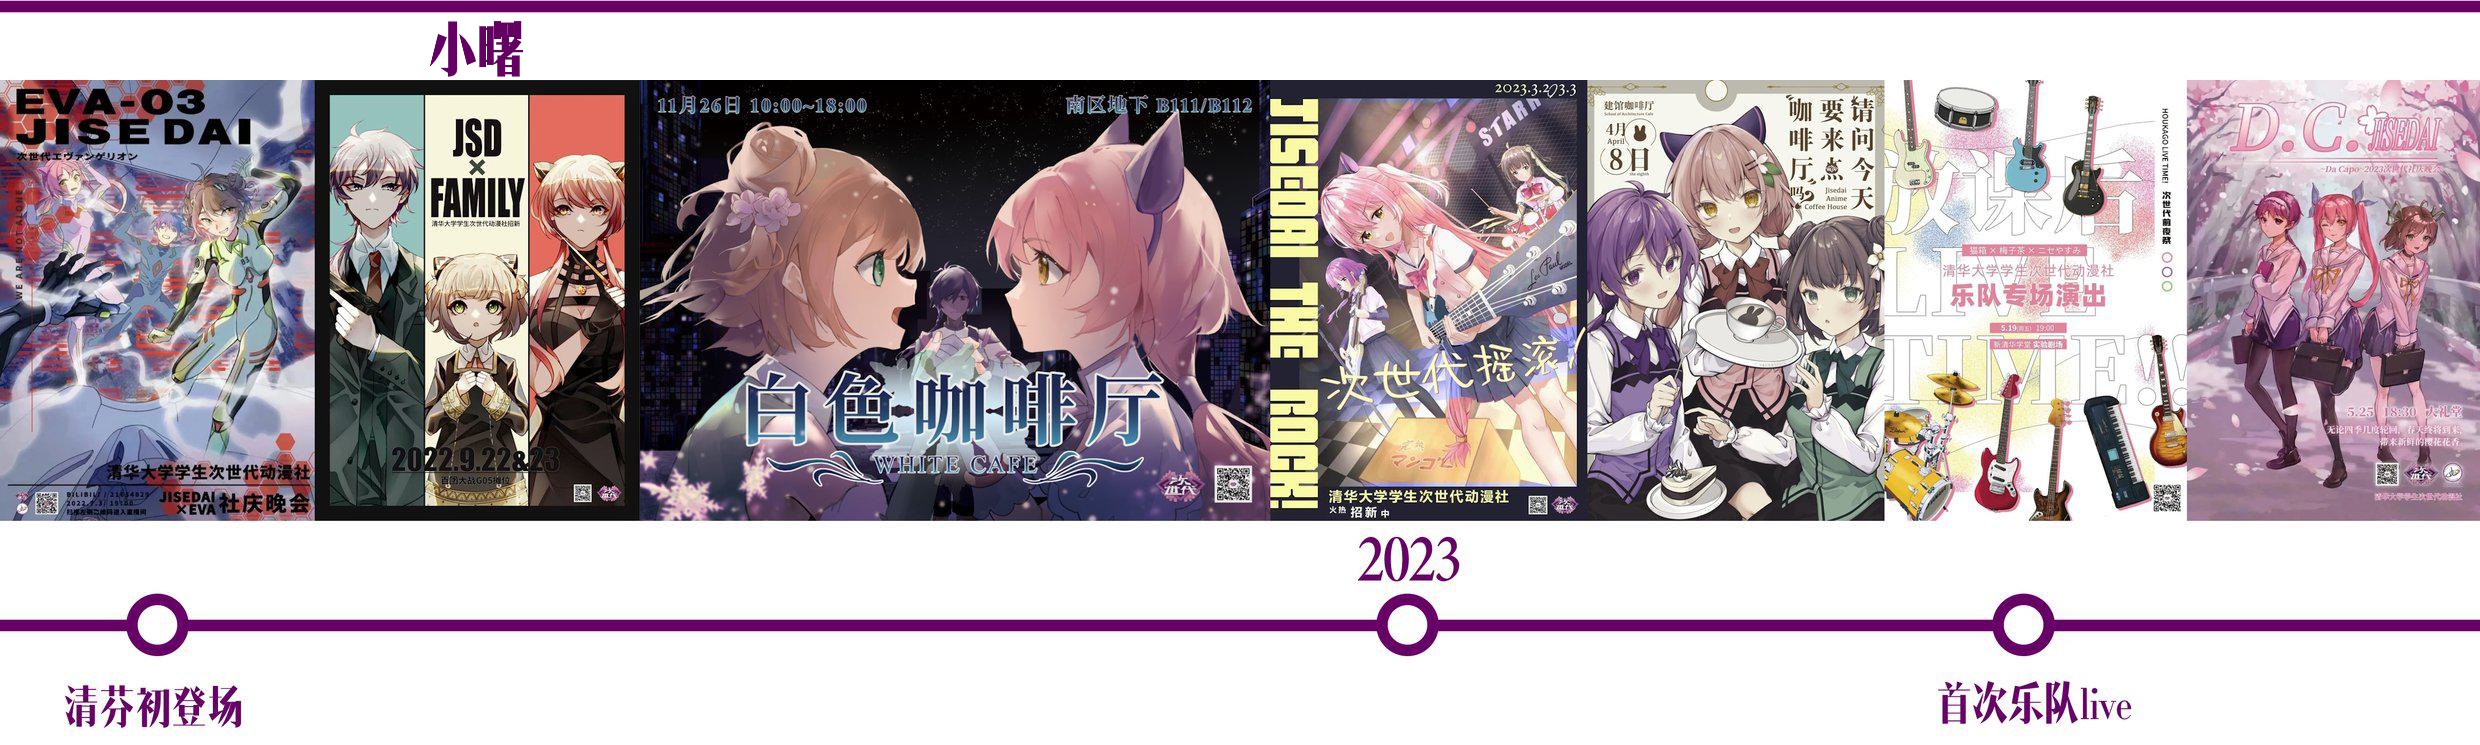
\includegraphics[width=\paperwidth]{tl5.jpg}
\end{textblock*}



\newpage
\fontsize{23pt}{24pt}\selectfont
\begin{center}
    \textbf{\textcolor{truepurple}{Idolive系列宅舞专场}}\\
\end{center}
\vspace{-0.5em}
\adjustbox{valign=t}{
	\begin{minipage}[t]{0.45\textwidth}
		\vspace{0.5em}
		\raisebox{-\height}{
			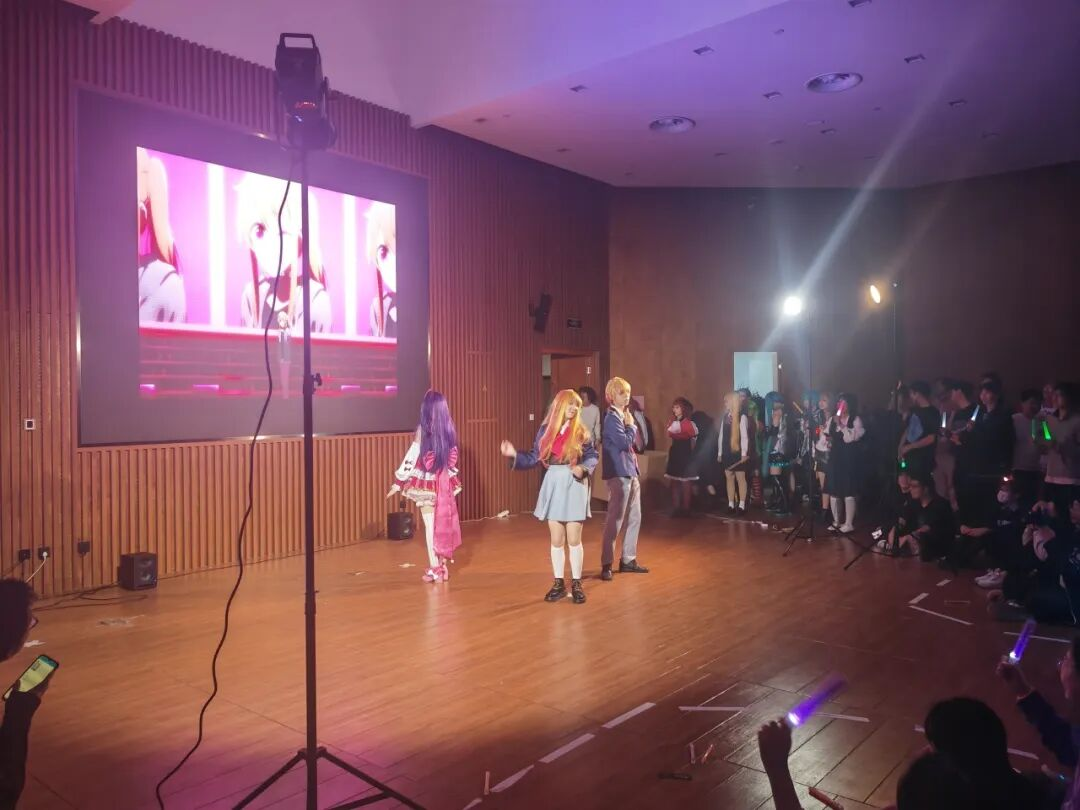
\includegraphics[width=\linewidth]{宅舞1.jpg}}
    \par
		\vspace{0.5em}
		\raisebox{-\height}{
			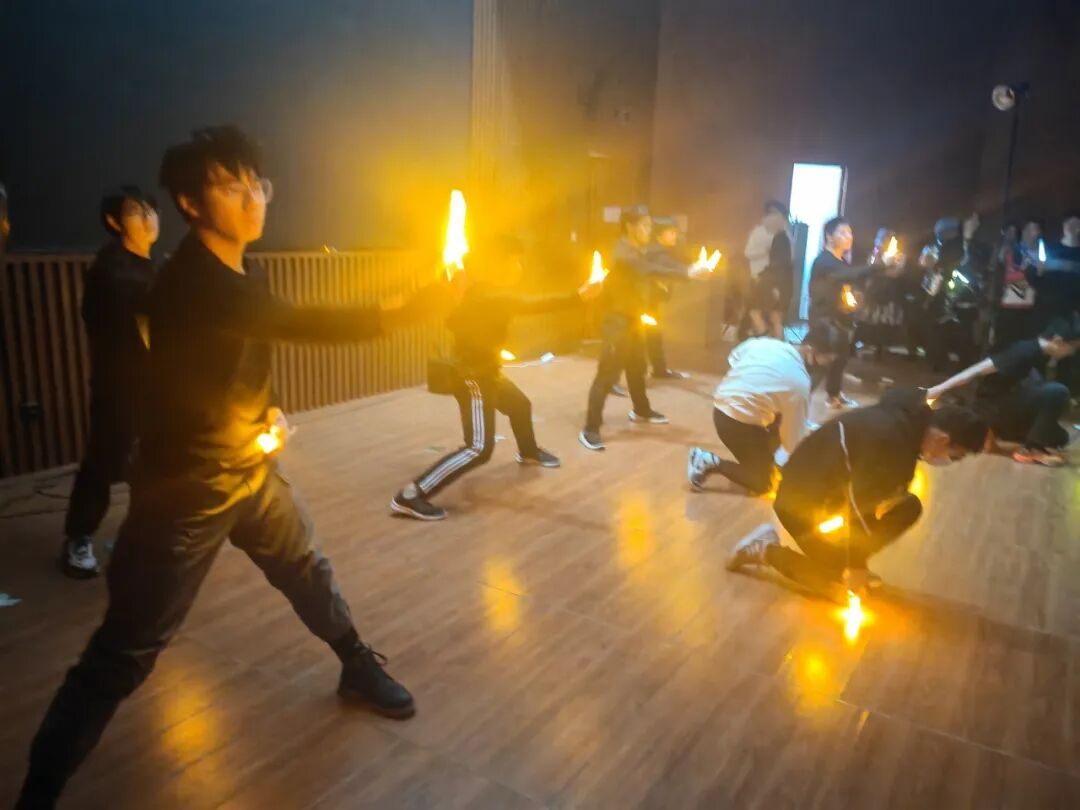
\includegraphics[width=\linewidth]{宅舞7.jpg}}
		\par
		\vspace{0.5em}
		\raisebox{-\height}{
			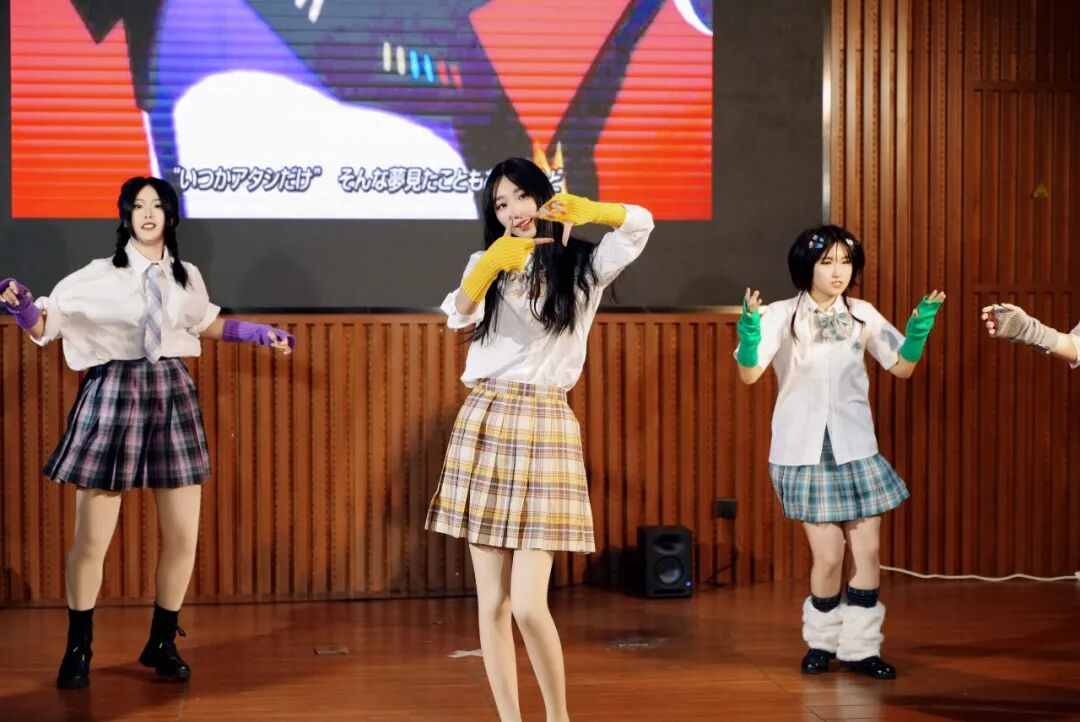
\includegraphics[width=\linewidth]{宅舞6.jpg}}

	\end{minipage}}
\hfill
\vspace{-0.5em}
\adjustbox{valign=t}{
	\begin{minipage}[t]{0.45\textwidth}
		\normalsize
    \par
		\chind Idolive系列是由次世代动漫社宅舞部自主研发的一款宅舞专场活动。专场发生在一个被称作B226的南区地下活动室,在这里,你将扮演超级元气小偶像,在自由的舞蹈中邂逅性格各异、能力独特的朋友们,逐步发掘宅舞的真相。清芬和桃子都曾经当过c位!\\
    \chind 宅舞专场分多段进行,中间设置了随机宅舞环节,随机串烧播放征集的配乐,可以自由登台下台,主打一个「想跳你就来」!\\
    \chind 此外, WOTA 艺部也会献上热血沸腾的光棒节目和应援。\\
		\par
    \vspace{-2em}
		\raisebox{-\height}{
			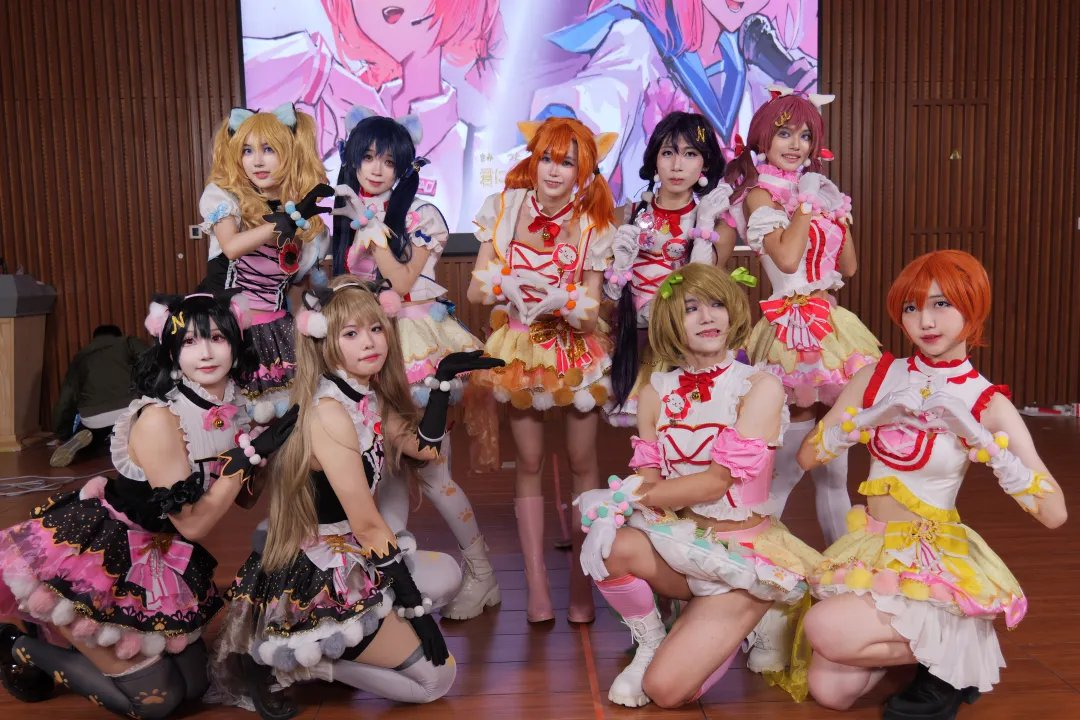
\includegraphics[width=\linewidth]{宅舞2.jpg}}

		\par
		\vspace{0.5em}
		\raisebox{-\height}{
			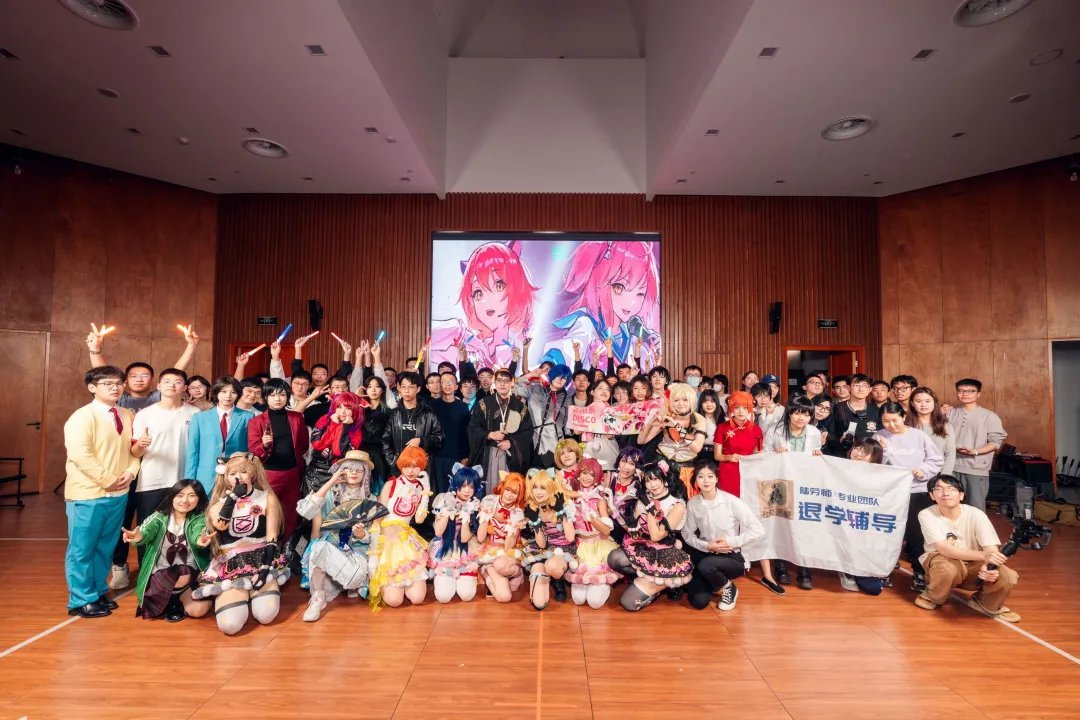
\includegraphics[width=\linewidth]{宅舞4.jpg}}

	\end{minipage}%
}
\begin{textblock*}{\paperwidth}(0mm, \dimexpr\paperheight-78.5mm\relax) % 距顶部 = 纸高 - 30mm
  \noindent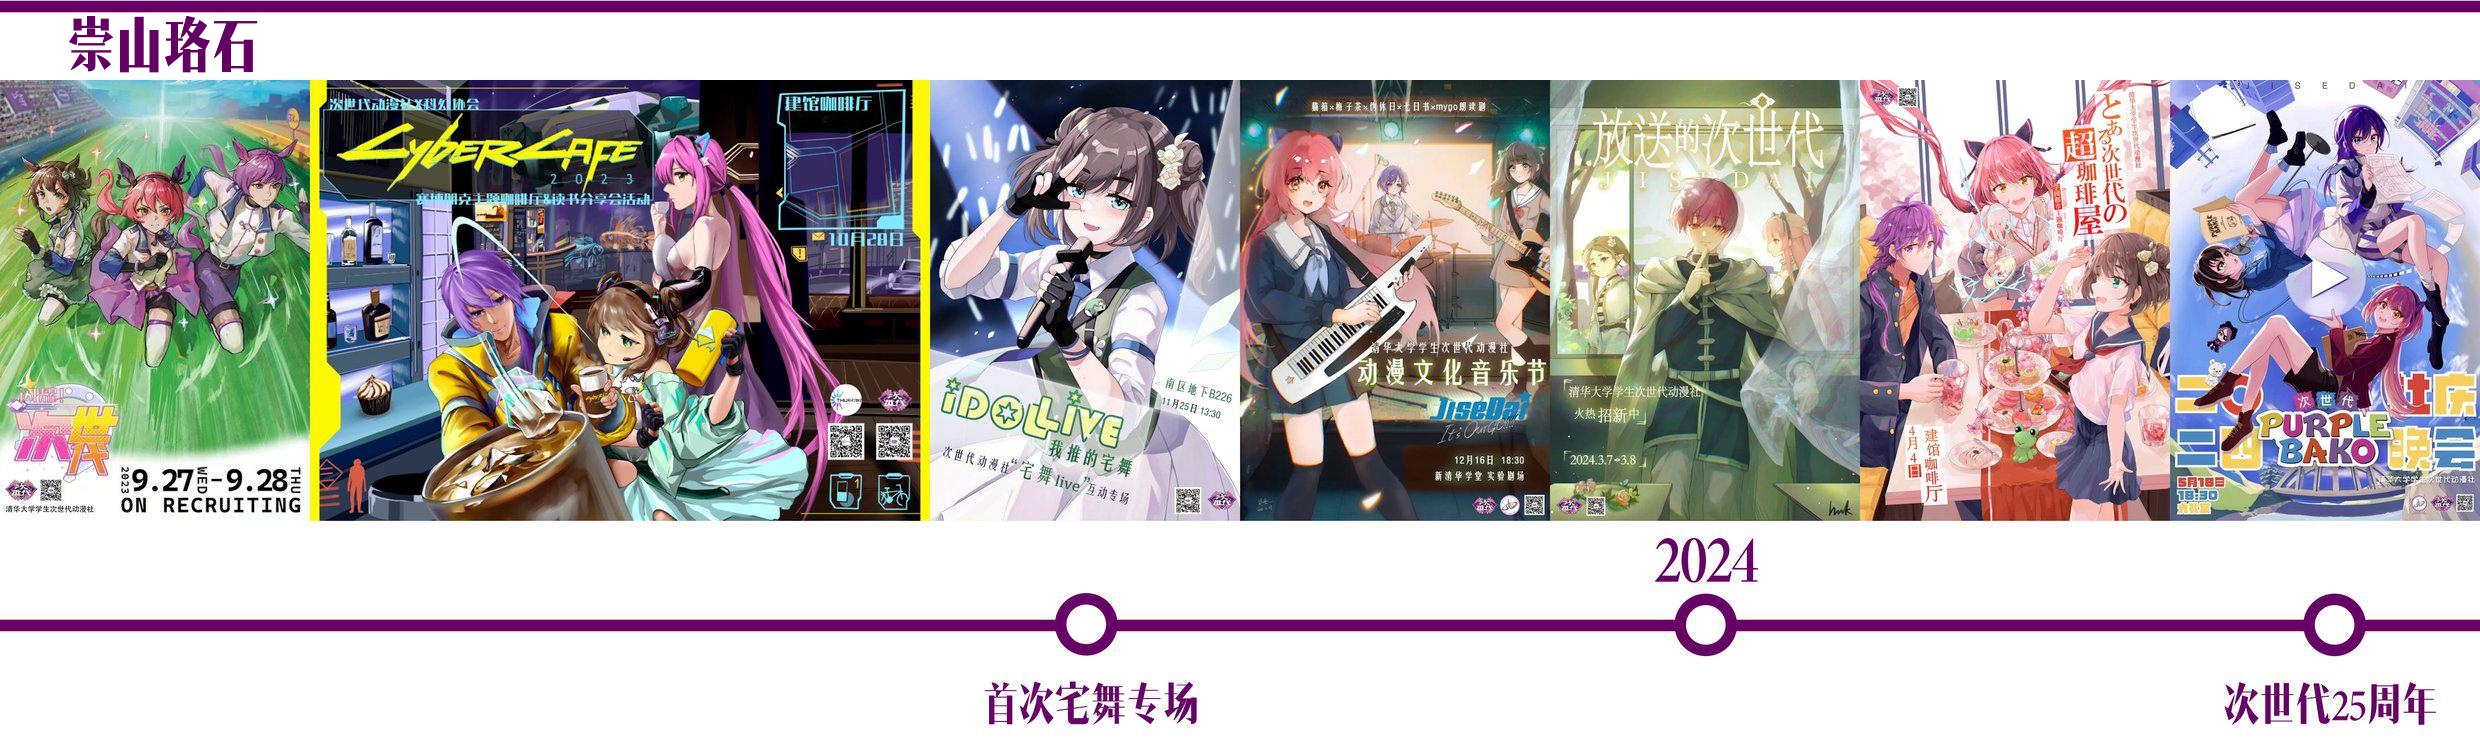
\includegraphics[width=\paperwidth]{tl6.jpg}
\end{textblock*}
\newpage
\par
\vspace{2em}

\adjustbox{valign=t}{
	\begin{minipage}[t]{0.4\textwidth}
		\vspace{-0.2em}
		\raisebox{-\height}{
			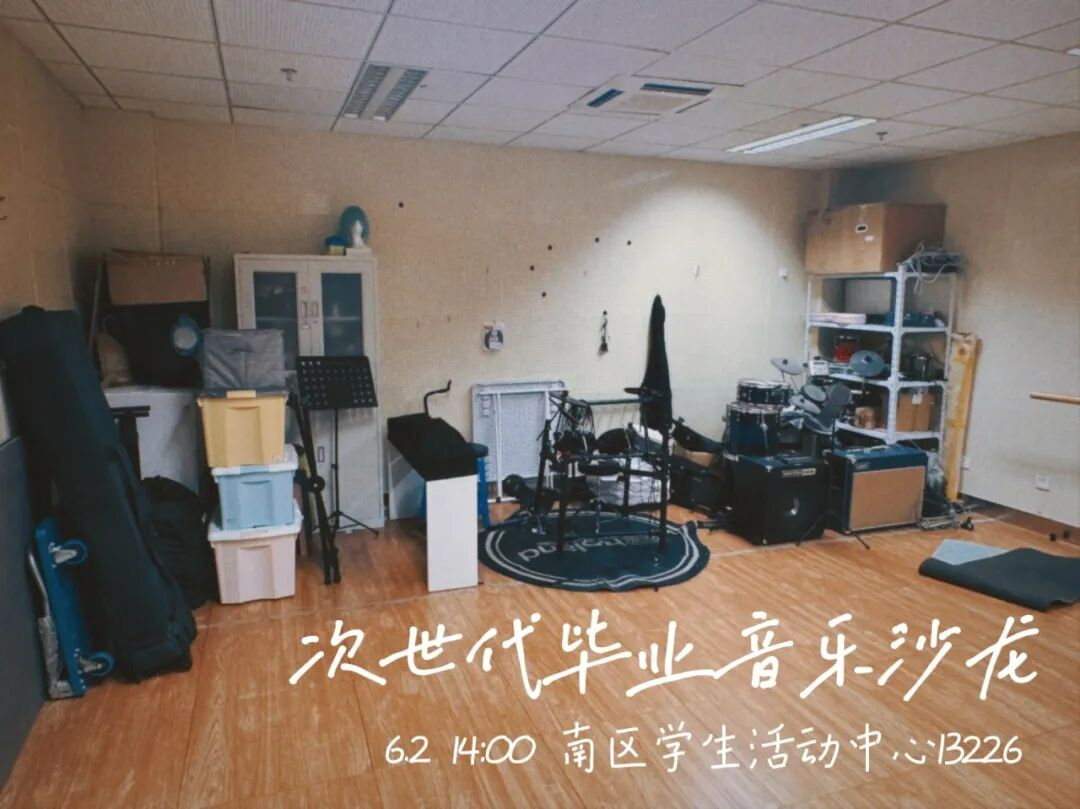
\includegraphics[width=1.1\linewidth]{沙龙.jpg}}
      \par
		\vspace{0.6em}
		\raisebox{-\height}{
			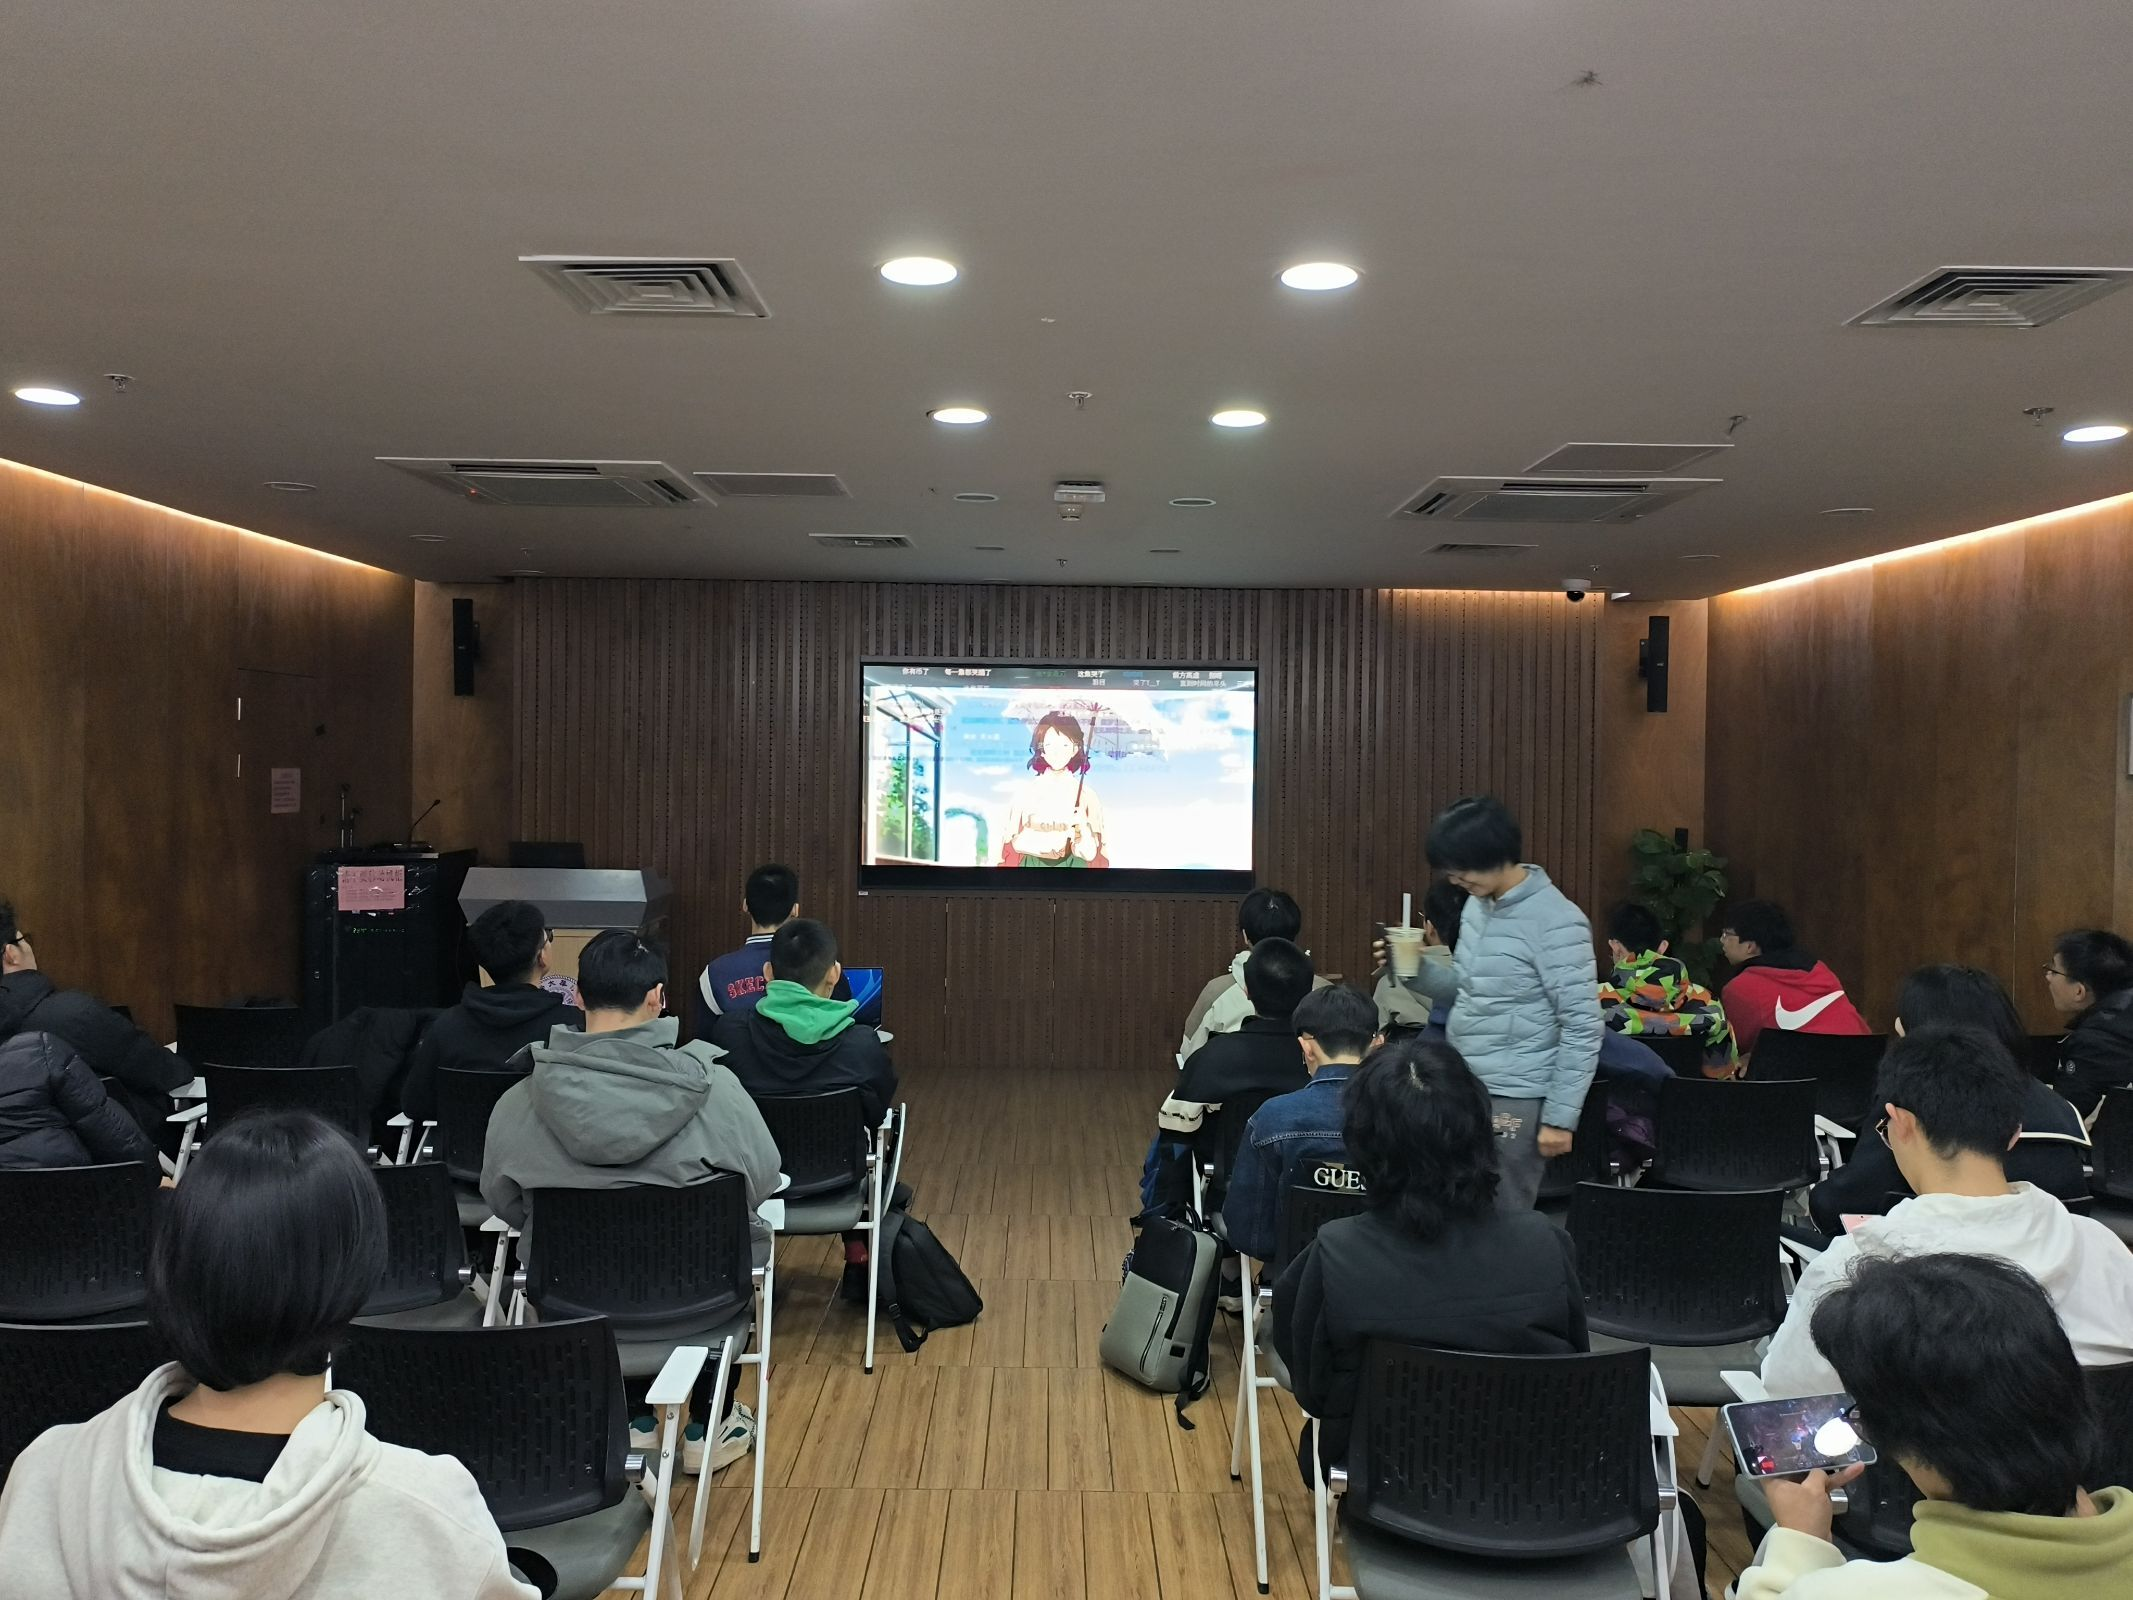
\includegraphics[width=1.1\linewidth]{放映会.jpg}}
      \par
		\vspace{0.6em}
		\raisebox{-\height}{
			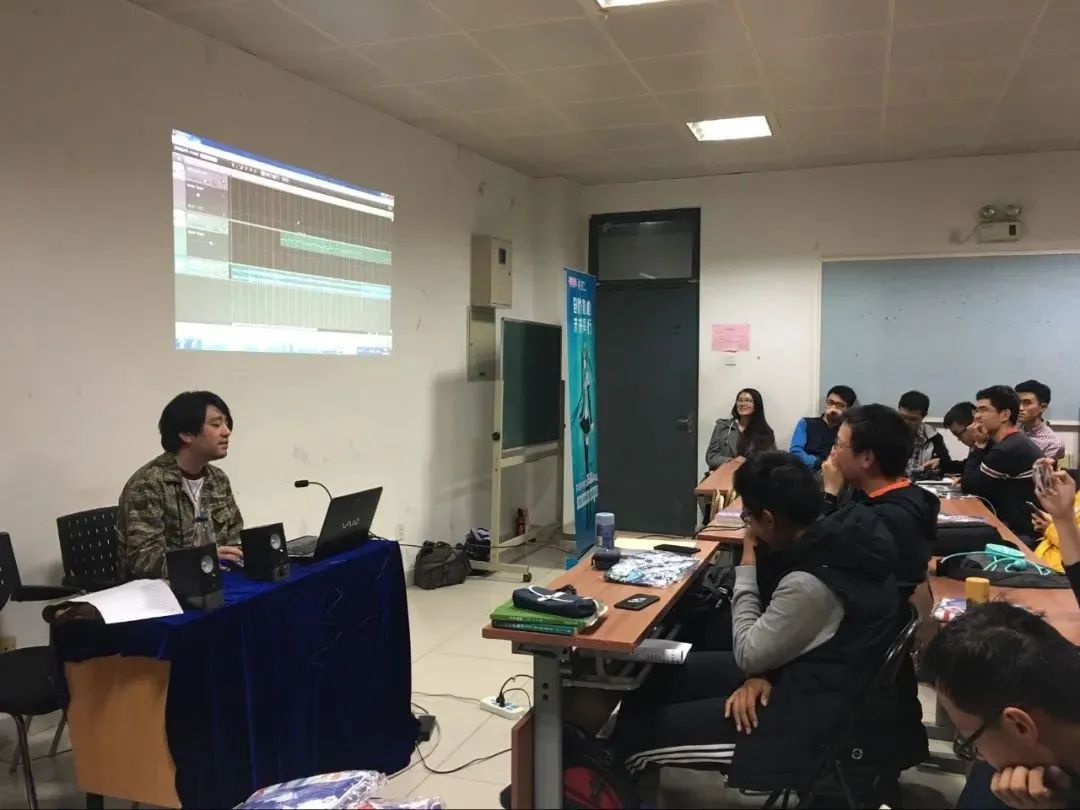
\includegraphics[width=1.1\linewidth]{讲座.jpg}}
	\end{minipage}%
}
\hfill
\adjustbox{valign=t}{
	\begin{minipage}[t]{0.5\textwidth}
    \fontsize{23pt}{24pt}\selectfont
    \begin{center}
\textbf{\textcolor{truepurple}{B226乐队部沙龙}}\\
    \end{center}
\par
		\vspace{-0.5em}
		\normalsize
		\chind 首次乐队部沙龙于上学期期末举办,主题为毕业季纪念,后续乐队部计划将该活动转化为常规活动。\\
    \chind 乐队部沙龙将以更轻松的氛围接纳更多的音乐元素,届时部内的临时企划和新手乐队将与大家见面,还会有anikura、现场点唱等活动等你到来。\\
   \par
    \fontsize{23pt}{24pt}\selectfont
    \vspace{-0.5em}
    \begin{center}
\textbf{\textcolor{truepurple}{周常放映会}}\\
    \end{center}
\par
		\vspace{-0.5em}
		\normalsize
		\chind 我们会在学期内每周开展经典动画电影,新剧场版动画或演唱会的放映活动,并建立了次世代放映组,为大家带来更好的观影体验。\\
    \chind 许多部门也会合作开展自己的放映。如果想要向同学安利你的品味\sout{公屏私用},欢迎加入放映组!\\
    \par
    \fontsize{23pt}{24pt}\selectfont
    \begin{center}
\textbf{\textcolor{truepurple}{例会/讲座}}\\
    \end{center}
\par
		\vspace{-0.5em}
		\normalsize
		\chind 例会是次世代\sout{除水群之外}的主要日常活动,其中分部例会更是重要的组成部分。虽然大家的兴趣各不相同,但总有一款能让你与同好们交流,结识更多同道中人。\\
    \chind 我们也经常邀请业界大佬来举办零距离讲座。先前邀请了知名Vocaloid~~P主匹诺曹P和知名插画师丁丁框老师,都获得了热烈反响,日后也敬请期待!\\
	\end{minipage}
}
\begin{textblock*}{\paperwidth}(0mm, \dimexpr\paperheight-78.5mm\relax) % 距顶部 = 纸高 - 30mm
  \noindent\includegraphics[width=\paperwidth]{tl7.jpg}
\end{textblock*}
\newpage
    \fontsize{23pt}{24pt}\selectfont
    \begin{center}
\textbf{\textcolor{truepurple}{往期活动}}\\
    \end{center}
    \par
\adjustbox{valign=t}{
	\begin{minipage}[t]{0.45\textwidth}
		
		\raisebox{-\height}{
			\includegraphics[width=\linewidth]{新年联欢晚会.jpg}}
		\vspace{-0.5em}
		\picbox{\small \ding{115} 出演新年联欢晚会}
  		\par
		\vspace{-0.5em}
		\raisebox{-\height}{
			\includegraphics[width=\linewidth]{舞萌.jpg}}
		\vspace{-0.5em}
		\picbox{\small ~\ding{115} ~ 舞萌DX比赛~}
	\end{minipage}}
\hfill
\vspace{1em}
\adjustbox{valign=t}{
	\begin{minipage}[t]{0.45\textwidth}
		\par
    
		\raisebox{-\height}{
			\includegraphics[width=\linewidth]{合宿.jpg}}
		\vspace{-0.5em}
		\picbox{\small ~\ding{115} ~ 合宿(会复刻的!)~}
		\normalsize
    \par
		\vspace{0em}
		\raisebox{-\height}{
			\includegraphics[width=0.8\linewidth]{BHCC.jpg}}
		\vspace{-0.5em}
		\picbox{\small ~\ding{115} ~ 参与BHCC北京高校联盟漫展~}

	\end{minipage}%
}
\normalsize
\chatbubble[right]{zijing.jpg}{紫荆}{
\textbf{甚至是,你想要举办的全新活动……?}
}{zi}
\begin{textblock*}{\paperwidth}(0mm, \dimexpr\paperheight-78.5mm\relax) % 距顶部 = 纸高 - 30mm
  \noindent\includegraphics[width=\paperwidth]{tl8.jpg}
\end{textblock*}  % 第二章:主要活动介绍
%\clearpage
\newpage % 开始新的一页
    \thispagestyle{empty} % 移除本页的页眉和页脚[8,9](@ref)
    \newgeometry{margin=0pt} % 临时将本页的页边距全部设置为0[1](@ref)
    \noindent % 防止缩进
    \includegraphics[width=0.9999\paperwidth, height=0.9999\paperheight]{ch3.png} % 插入图片,使其尺寸与纸张大小一致并保持宽高比[1](@ref)
    \restoregeometry % 恢复原来的页边距设置

\chatbubble[left]{qiya.jpg}{奇犽}{
 次世代有哪些活动?
}{default}

\chatbubble[right]{taozi.png}{桃子}{
 次世代的活动真的超级多!常驻活动有每年一次的社庆晚会,每学期一次主题咖啡厅、
 乐队live、宅舞专场演出,以及各分部自发组织的活动,如绘画部的茶绘、动研部的新番研讨会、
 地下live部的应援例会、东方部的东方例会、Lolita部的茶话会、各个二游部的集体赌博
 (给赌博来个划掉的效果)抽卡等等;此外还会不定期掉落一些大牛的讲座分享
 (已经建设过丁丁框大大和匹诺曹大大了!)、圣诞例会、配音演员见面会等等。
 未来还会有更多的活动需要由你们来建设,快来和桃子一起搞波大的吧!
}{tao}

\chatbubble[left]{guitarhero.png}{吉他英雄}{
  加入动漫社……是不是意味着要参加好多好多线下活动?要自我介绍?要上舞台?
  这个绝对做做做做做做做做不到!
}{default}

% 右侧聊天(用户B)
\chatbubble[right]{qingfen.png}{清芬}{
 绝对没这回事~我们所有的活动都是自愿参加的!当然,我们欢
 迎每一位社员的热情。但是就算只是来咖啡厅买一杯特调,来社庆做
 一枚静静的观众,或在群聊里默
 默收集好看的图片也都没问题!我们的宗旨就是玩得开心~
}{qing}

\chatbubble[left]{zijing.png}{紫荆(四肢驯服中)}{
 不会跳舞可以加入宅舞部吗。?
}{zi}

\chatbubble[right]{taozi.png}{桃子}{
 当然可以!宅舞部很多都是0基础的朋友噢~只要热爱就可以加入,
 大家会一起学舞一起练习的(抱大腿)喜欢您来!
}{tao}

\chatbubble[left]{mortis.png}{若叶睦(Mortis 版)}{
 想加入创作部门,但无论乐队还是绘画、cosplay、宅舞,全~都不会!
}{default}

\chatbubble[right]{qingfen.png}{清芬}{
 没关系,大部分人都和你一样!正是因此,几乎每个创作部门招新时都会强调:
 我们部门从不拒绝零基础选手,我们有热心太太组成的资深团队,帮助每个虚心求教的萌新快速入门!
}{qing}

\newpage

\chatbubble[left]{konami.png}{(该用户未填写昵称)}{
 我的品味小众又独特,该如何在次世代找到同好呢?
}{default}

\chatbubble[right]{taozi.png}{桃子}{
 次世代最不缺的就是小众作品爱好者(此处应有一张部门全表),只要多水群,找不到同好比找到同好还难呢!
 此外,我们秉承“三人成部”传统,只要再有两位同好,就可以申请成立一个新部门~如果你有感兴趣的领域
 还没有部门,欢迎来找我们哦!
}{tao}

\chatbubble[left]{shishangyou.png}{冻鳗领域大神}{
 如何向大家推荐我喜欢的作品?
}{default}

\chatbubble[right]{zijing.png}{紫荆}{
 有很多种方式。次世代动画研究会(简称动研部)会定期举办新番研讨会,这是安利作品、分享见解的最好机会。
 此外,次世代放映组每周都会组织放映会,现在加入放映部,完成登记和教室预约后,就可以申请放映自己喜欢的作品了。
}{zi}

\chatbubble[left]{wohenhaoqi.png}{好奇宝宝}{
 我也想为次世代的活动出一份力,我该如何成为帕鲁?
}{default}

\chatbubble[right]{qingfen.png}{清芬}{
 次世代组织部欢迎你的加入!组织部每周都会举办例会,分配下一周的工作任务。
 值得一提的是,所有任务都是自愿接受的,例会只来旁听也完全没问题~
 在主题咖啡厅、社庆等大型活动前,组织部群里还会发布志愿者招募公告,填写问卷后就可以成为帕鲁啦!
 大型活动的帕鲁可能还会有神秘福利哦~
}{qing}

\chatbubble[left]{rika.png}{极东魔术昼寝结社の夏社长}{
 次世代会和其他社团合作举办活动吗?
}{default}

\chatbubble[right]{zijing.png}{紫荆}{
 时常会有。次世代放映部不时会和学生科幻协会合作举办科幻电影放映会;主题咖啡厅也是外社
 联动的常客,荷月玩偶社、学生科幻协会等都曾是我们的联动对象。此外,学生电子音乐协会、学生推理协会
 也曾和我们有过合作。如果有任何想要进行外社联动的想法,欢迎联络组织部。
}{zi}  % 第三章:社团Q&A
%\clearpage
\newpage % 开始新的一页
    \thispagestyle{empty} % 移除本页的页眉和页脚[8,9](@ref)
    \newgeometry{margin=0pt} % 临时将本页的页边距全部设置为0[1](@ref)
    \noindent % 防止缩进
    \includegraphics[width=0.9999\paperwidth, height=0.9999\paperheight]{ch4.png} % 插入图片,使其尺寸与纸张大小一致并保持宽高比[1](@ref)
    \restoregeometry % 恢复原来的页边距设置
\arial
\newpage
\fontsize{23pt}{24pt}\selectfont
\textbf{\textcolor{truepurple}{次世代组织部}}\\
\vspace{0.7em}
\adjustbox{valign=t}{
	\begin{minipage}[t]{0.37\textwidth}
		\vspace{-0.5em}
		\raisebox{-\height}{
			\includegraphics[width=\linewidth]{组织部.png}}
		\picbox{\small ~~\ding{115} ~ 组织部酱~}
	\end{minipage}%
}
\hfill
\adjustbox{valign=t}{
	\begin{minipage}[t]{0.53\textwidth}
		\normalsize
		\chind 组织部是次世代唯一的管理部门,是由自愿处理次世代部门事务、
		为次世代而发光发热的社友组织而成的。\\
        \chind 组织部基本会在每周末择时择地开一次线下例会,例会向全体社员开放,
		用于讨论近期需要组织部参与组织工作的次世代活动事宜。参与例会是加入组织部工作的直接方式,
		例会的氛围轻松、节奏快,非常适合新人快速熟悉次世代内部情况、并快速交到新朋友,\sout{从而走对大学第一条路并走上人生巅峰}。\\
		\chind 财务、宣传、外联、舞监是组织部主要下属职务,
		并各自有一个工作组来处理相关事务。财务负责提供活动资金和统计收入支出,
		宣传主要是运营社内公众号和b站账号等,负责同步社内信息和对外打造社团形象,
		外联负责同其他社团(尤其是其他学校动漫社)、赞助方等进行对接,
		舞监负责舞台节目的审核、推进。
		工作组的分工和准入比较自由,每个人都能从中找到适合自己的位置。\\
	\end{minipage}
}
\adjustbox{valign=t}{
	\begin{minipage}[t]{0.45\textwidth}
		\normalsize
		\vspace{-0.7em}
		\chind 在举办社内活动时,组织部成员通常充当活动staff的角色,
		此外也会面向整个社团招募staff。成为活动staff是熟悉组织部工作方式的好途径\sout{还能品尝到工作餐五道双马。}\\
		\chind 组织部的初衷是服务社内同好人群,如果你有新颖又务实的想法,欢迎向组织部提出,组织部会尽可能帮你实现梦想。同时欢迎来到组织部助力他人的梦想\sout{当帕鲁},共同打造一个繁荣的次世代!\\


	\end{minipage}
}
\hfill
\adjustbox{valign=t}{
	\begin{minipage}[t]{0.45\textwidth}
		\vspace{-0.5em}
		\raisebox{-\height}{
			\includegraphics[width=\linewidth]{组织部3.png}}
		\vspace{-0.7em}
		\picbox{\small ~\ding{115} ~~ 组织部例会为友校动漫社录制祝福}
	\end{minipage}%
}

\adjustbox{valign=t}{
	\begin{minipage}[t]{0.45\textwidth}
		\vspace{-0.5em}
		\raisebox{-\height}{
			\includegraphics[width=\linewidth]{组织部1.png}}
		\vspace{-0.7em}
		\picbox{\small \ding{115} ~ 2025社庆staff合影~}
	\end{minipage}%
}\adjustbox{valign=t}{
	\begin{minipage}[t]{0.45\textwidth}
		
		\raisebox{-\height}{
			\includegraphics[width=1.1\linewidth]{组织部2.png}}
		\vspace{-0.7em}
		\picbox{\small ~~\ding{115} ~ 次世代x幻协~“次元穿越”社会实践~}
	\end{minipage}%
}
%——————————————创作类——————————————%
% 绘画部
%
%

\newpage
\fontsize{23pt}{24pt}\selectfont
\textbf{\textcolor{truepurple}{次世代绘画部}}
\hfill
\fontsize{19pt}{20pt}\selectfont
\textbf{\textcolor{truepurple!70!white}{—————创作类}}\\
\vspace{0.7em}
\adjustbox{valign=t}{
	\begin{minipage}[t]{0.22\textwidth}
		\vspace{-0.5em}
		\raisebox{-\height}{
			\includegraphics[width=\linewidth]{部酱/绘画部.png}}
		\vspace{-0.5em}
		\picbox{\small ~~\ding{115} ~ 绘画部酱~}
	\end{minipage}%
}
\hfill
\adjustbox{valign=t}{
	\begin{minipage}[t]{0.68\textwidth}
		\normalsize
		\chind 你想在大学时光里尽情挥洒自己的绘画创造力吗,来绘画部就对了!这里不仅有画技点满的太太,也有刚开始接触绘画的小白,不管你是想提高画技还是画同人还是造oc,抑或绘制海报和参加原创本,在这里都有属于你的一片天地。\\
		\chind 绘画部的活动包括但不限于线上活动:画图发图传相册、复读水群、夸夸或者被夸夸、不同形式的绘画接龙、出同人本,不过这些都是线上活动,说到线下活动当然少不了茶绘!大家可以带上自己的设备和工具,来线下面基聊天画画,还可以玩
		桌游,总之是十分欢乐的活动!\\
	\end{minipage}
}
\par
\vspace{0.5em}
\adjustbox{valign=t}{
	\begin{minipage}[t]{0.6\textwidth}
		\normalsize
		\chind 如果你想要在群内展示自己的作品,可以自行创建属于自己的群相册~方便大家夸夸!\\
		\chind 绘画部在社团主视觉的绘制上也有十分悠久的历史了,就连大家熟知的rella蘑菇太太也在绘画部为动漫社画过活动海报,机会多多,大家可以毛遂自荐!

	\end{minipage}
}
\hfill
\adjustbox{valign=t}{
	\begin{minipage}[t]{0.35\textwidth}
		\vspace{-2.5em}
		\raisebox{-\height}{
			\includegraphics[width=\linewidth]{绘画部1.png}}
		\vspace{-0.8em}
		\picbox{\small ~~\ding{115} ~ 某次茶绘现场~}
	\end{minipage}%
}
\adjustbox{valign=t}{
	\begin{minipage}[t]{0.3\textwidth}

		\raisebox{-\height}{
			\includegraphics[width=\linewidth]{绘画部2.png}}
		\vspace{-0.5em}
		\picbox{\small \ding{115} ~ Vocaloid展摆摊~}
	\end{minipage}%
}  \adjustbox{valign=t}{
	\begin{minipage}[t]{0.65\textwidth}
		\vspace{1em}
		\normalsize
		\chind 总而言之,在绘画部这个温暖的集体里,大家可以尽情交流有关绘画的问题,
		群内也有着十分珍贵的学习资料(正经)供大家学习,也可以在这里寻找同担,
		共同交流互绘oc同人,时不时吃吃群里其他太太做出香香的饭,请感兴趣的同学加入吧!\\
		\chind(ps:群内禁发涩图和ai图,讨论ai绘画请移步别处)

		\raisebox{-\height}{
			\includegraphics[width=0.9\linewidth]{绘画部3.png}}
		\picbox{\small ~~\ding{115} ~ 某次茶绘产出~}
	\end{minipage}%
}
%
%
% cosplay舞台剧部
%
%
\newpage
\fontsize{23pt}{24pt}\selectfont
\textbf{\textcolor{truepurple}{次世代cosplay舞台剧部}}
\\
\vspace{0.7em}
\adjustbox{valign=t}{
	\begin{minipage}[t]{0.25\textwidth}
		\vspace{-0.5em}
		\raisebox{-\height}{
			\includegraphics[width=\linewidth]{部酱/cosplay舞台剧.png}}
		\picbox{\small ~~\ding{115} ~ cosplay舞台剧部酱~}
	\end{minipage}%
}
\hfill
\adjustbox{valign=t}{
	\begin{minipage}[t]{0.65\textwidth}
		\normalsize
		\chind 大家好啊,这里是cosplay舞台剧部!\\
		\chind 顾名思义,这里既有cosplay,又有舞台剧———是并集而不是交集。\\
		\chind 部门的活动有许多,包括最盛大的社庆舞台剧节目、百团大战出cos、在动漫咖啡厅活动出cos、约漫展、约团片、约计划、约饭……\\
		\chind 社庆的舞台剧节目上,我们有19年的命运石之门,21年的方舟走秀,24年的逆转裁判和25年的“苹果默示录”。\\
		\chind 在百团大战中,社团会约好c楼的活动室方便大家化妆,一起在摊位上出cos也不社恐。在动漫主题咖啡厅中,我们还会设置符合主题的布景,让大家拍照使用。\\
		\chind 大家可以组团去方舟ONLY、V家ONLY等漫展。\\
	\end{minipage}
}
\adjustbox{valign=t}{
	\begin{minipage}[t]{0.65\textwidth}
		\normalsize
		\chind 约团片约计划什么的,只需要在群里说一声。万一成功了呢!这组JOJO黄金之风团片仅仅起源于一句话。并且结束以后一起去吃了披萨。\\
		\chind 没出过cos,怎么办?尽管在群里提出问题吧!群内也有技术高超的妆娘、毛娘老师。试着在部门活动中迈出cosplay的第一步。\\
		\chind 总之,欢迎所有对此有兴趣的同学加入!
		\\
	\end{minipage}
}
\hfill
\adjustbox{valign=t}{
	\begin{minipage}[t]{0.25\textwidth}
		\vspace{-0.5em}
		\raisebox{-\height}{
			\includegraphics[width=\linewidth]{cos部3.png}}
		\vspace{-0.7em}
		\picbox{\small ~~\ding{115} ~ JOJO黄金之风团片~}
	\end{minipage}%
}
\adjustbox{valign=t}{
	\begin{minipage}[t]{0.45\textwidth}
		\vspace{-2.5em}
		\raisebox{-\height}{
			\includegraphics[width=\linewidth]{cos部1.png}}
		\vspace{-0.7em}
		\picbox{\small \ding{115} ~ 2024咖啡厅coser合影~}
	\end{minipage}%
}  \adjustbox{valign=t}{
	\begin{minipage}[t]{0.45\textwidth}
		\vspace{0.5em}
		\raisebox{-\height}{
			\includegraphics[width=1.1\linewidth]{cos部2.png}}
		\vspace{-0.7em}
		\picbox{\small ~~\ding{115} ~ 2024社庆舞台剧《逆转裁判》~}
	\end{minipage}%
}
%——————————————歌舞艺术类————————————%
%
%
% 宅舞部
%
%
\newpage
\fontsize{23pt}{24pt}\selectfont
\textbf{\textcolor{truepurple}{次世代宅舞部}}
\hfill
\fontsize{19pt}{20pt}\selectfont
\textbf{\textcolor{truepurple!70!white}{—————歌舞艺术类}}\\
\vspace{2em}
\adjustbox{valign=t}{
	\begin{minipage}[t]{0.65\textwidth}
		\normalsize
		\chind 嗨嗨!这里是次世代宅舞部! \\
		\chind 在这里,你可以找到手把手教学的同学、一起练习表演的同伴、吃喝玩乐的朋友…… 
		我们为大家提供各样的平台:宅舞专场、社庆、BDF……还有清社派对、百团大战等学校舞台,
		还会随机掉落学生节、跨年晚会、外校联动等机会。\\
	\end{minipage}
}
\hfill
\adjustbox{valign=t}{
	\begin{minipage}[t]{0.3\textwidth}
		\vspace{-1em}
		\raisebox{-\height}{
			\includegraphics[width=0.9\linewidth]{宅舞部.png}}\hspace*{\fill}
		\picbox{\small ~~\ding{115} ~ 宅舞部酱~}
	\end{minipage}%
}
\adjustbox{valign=t}{
	\begin{minipage}[t]{0.45\textwidth}
		\vspace{-4.05em}
		\raisebox{-\height}{
			\includegraphics[width=\linewidth]{宅舞部1.png}}
		\vspace{-0.8em}
		\picbox{\small ~~\ding{115} ~ 宅舞专场精彩舞台~}
		\par
		\vspace{-1em}
		\raisebox{-\height}{
			\includegraphics[width=\linewidth]{宅舞部2.png}}
		\vspace{-0.8em}
		\picbox{\small \ding{115}  Lovelive $\mu 's$舞团}
		\par
		\vspace{-1em}
		\raisebox{-\height}{
			\includegraphics[width=\linewidth]{宅舞部3.png}}
		\vspace{-0.8em}
		\picbox{\small \ding{115}  如此幸福初代专场}
	\end{minipage}%
}
\hfill
\adjustbox{valign=t}{
	\begin{minipage}[t]{0.45\textwidth}
		\normalsize
		\vspace{0.8em}
		\chind 日常也会有排练室提供!录制视频和外出爬台也更加便利! 除了跳舞之外,我们还有丰富多彩的团建活动!海底捞、萨莉亚……(还会有神秘二创活动x) \\
		\chind 选择您的音乐,组建您的舞团,次世代大舞台,欢迎您来! 和宅舞部酱一起kirakira吧!
		\raisebox{-\height}{
			\includegraphics[width=\linewidth]{宅舞部4.png}}
		\vspace{-0.8em}
		\picbox{\small ~~\ding{115} ~ 2024 Bilibili Dancing Festival~}
		\par
		\vspace{-1em}
		\raisebox{-\height}{
			\includegraphics[width=\linewidth]{宅舞部5.png}}
		\vspace{-0.8em}
		\picbox{\small \ding{115}  2024社庆宅舞部合照}
	\end{minipage}
}

%
%
% 乐队部
%
%
\newpage
\fontsize{23pt}{24pt}\selectfont
\textbf{\textcolor{truepurple}{次世代乐队部}}\\
\vspace{0.7em}
\adjustbox{valign=t}{
	\begin{minipage}[t]{0.65\textwidth}
		\normalsize
		\vspace{-1em}
		\chind 乐队动画千万次,亲自组队第一次!\\
		\chind 次世代乐队部建群于2014年,其前身为翻奏ACGN曲目的鸡排饭乐队,
		在次世代社庆上留下过大量精彩瞬间。自2022年开始,该部门转型为集乐队组建与演出、
		技术交流、活动筹备等在内的综合型产出部门。现有乐队数目近10支,部内乐手储备超150人。\\
	\end{minipage}
}
\hfill
\adjustbox{valign=t}{
	\begin{minipage}[t]{0.3\textwidth}
		\vspace{-1.5em}
		\raisebox{-\height}{
			\includegraphics[width=1.1\linewidth]{乐队部.png}}\hspace*{\fill}
		\vspace{-0.5em}
		\picbox{\small ~~\ding{115} ~ 乐队部酱~}
	\end{minipage}%
}
\adjustbox{valign=t}{
	\begin{minipage}[t]{0.45\textwidth}
		\vspace{-5em}
		\raisebox{-\height}{
			\includegraphics[width=\linewidth]{乐队部2.png}}
		\vspace{-0.8em}
		\picbox{\small ~~\ding{115} ~ 2021年社庆乐队部视频节目~}
		\par
		\vspace{-1em}
		\raisebox{-\height}{
			\includegraphics[width=\linewidth]{乐队部1.png}}
		\vspace{-0.8em}
		\picbox{\small \ding{115}  参与《BanG Dream!》手游国服高校乐队联动活动}
	\end{minipage}%
}
\hfill
\adjustbox{valign=t}{
	\begin{minipage}[t]{0.45\textwidth}
		\normalsize
		\vspace{0.8em}
		\chind 部门的最大规模活动是每学期一次的乐队专场live,
		由部内各乐队为大家带来量大管饱的精彩现场。每学年的部门迎新会是新成员们结识彼此、
		寻找未来搭档的良好机会。此外,部门还会不定期掉落沙龙、路演等演出活动。\\
		\chind 在乐队部,你不仅能够得到一个研究演奏演唱、鉴赏各流派音乐、
		把玩乐器装备、交流组队心得的空间,更能让你成为自己的乐队故事主角。
	\end{minipage}
}
\includegraphics[width=\linewidth]{乐队部3.png}
\vspace{-2em}
\picbox{\small ~~\ding{115} ~ 部门人才储备共享文档~}\\
\normalsize
从十余年前的鸡排饭出发,下一曲即将奏响,\\
让我们一起期待在名为乐队的盛行风中飞得更远!
%
%
%wota艺部
%
%
\newpage
\fontsize{23pt}{24pt}\selectfont
\textbf{\textcolor{truepurple}{次世代水木wota艺部}}\\
\vspace{0.7em}
\adjustbox{valign=t}{
	\begin{minipage}[t]{0.3\textwidth}
		\vspace{-0.5em}
		\raisebox{-\height}{
			\includegraphics[width=1.15\linewidth]{WOTA艺.png}}
		\vspace{-0.5em}
		\picbox{\small ~\ding{115} ~ WOTA艺部酱~}
	\end{minipage}%
}
\hfill
\adjustbox{valign=t}{
	\begin{minipage}[t]{0.6\textwidth}
		\small
		\chind wota艺,又称光棒艺,是一项发源于偶像应援文化,发展为独立表演性质的舞蹈形式。
		其主要特征为“双脚基本固定,上肢大幅度运动,双手持光棒”。表演形式既可以是视频创作,也可以是舞台表演。\\
		\chind wota艺的美感来源于双手所创造出的光弧,以及动作与歌曲节奏的契合度。
		只要是你所喜爱的歌曲,就可以由你亲手设计编排,联系部员,带上光棒,
		一同对歌曲进行演绎。如果你对舞蹈,MV向视频创作,剪辑与后期感兴趣,
		我们欢迎你来探索wota艺这个全新的艺术创作领域。\\
		\chind 次世代水木wota艺部最早于2018年创立,自此每年社庆都有节目登台,
		从未缺席。同时,还参与了诸如社团嘉年华,学生节等多次全校范围的表演活动。
		与北大元火水月wota艺部常有合作,产出了大量舞台企划和视频企划。此外,
		与北交,北航,北外,中传等多校均有合作交流。
	\end{minipage}
}
\par
\vspace{0.5em}
\adjustbox{valign=t}{
	\begin{minipage}[t]{0.5\textwidth}
		\small
		\chind wota艺部具有丰富的每周常规活动:每周均有2~3次“光棒聚会”,一般在北体二层平台进行,会有手把手的光棒技术教学环节以及视频企划的录制。来时记得带上你最喜欢的歌单,我们会与你共同用光弧演绎!此外还有聚餐,KTV,合宿等项目不定时掉落!\\
		\chind 除了社庆以外,wota艺部在次世代宅舞专场和学生节都会有爬台企划,只要每周坚持参加周常,最终都能参与到企划中,登台表演,在聚光灯下展示自我。\\
		\chind 如果你对wota艺产生了浓厚的兴趣,想要进一步精进技术,每周末在中关村首钢大平台都有全北京范围的光棒聚会可供参加,可以与领域内最强大的wota艺打师交流学习。北京每年都有2到3次光棒比赛,欢迎参加,证明你的实力!\\
		\chind wota艺不仅是表演形式,同时也是一种健康的有氧运动,在锻炼肢体协调能力的同时,提高心肺功能,上肢与核心力量,治疗圆肩驼背,延年益寿,妙处无穷。\\
		\chind wota艺更是一种社交方式。在这里,你能找到动漫同好,游戏同好,拓宽交际圈,认识天南海北的朋友,共同享受创作的快乐。\\
		\chind 次世代水木wota艺部,欢迎您来!
	\end{minipage}}
\hfill
\vspace{1em}
\adjustbox{valign=t}{
	\begin{minipage}[t]{0.45\textwidth}
		\vspace{-0.5em}
		\raisebox{-\height}{
			\includegraphics[width=\linewidth]{wota艺部1.png}}
		\vspace{-0.5em}
		\picbox{\small ~\ding{115} ~ 软院学生节场照~}
		\begin{minipage}[t]{0.5\textwidth}
			\vspace{-0.5em}
			\raisebox{-\height}{
				\includegraphics[width=\linewidth]{wota艺部2.png}}
		\end{minipage}%
		\begin{minipage}[t]{0.5\textwidth}
			\vspace{-0.5em}
			\raisebox{-\height}{
				\includegraphics[width=\linewidth]{wota艺部3.png}}
		\end{minipage}%
		\vspace{-0.5em}
		\picbox{\small ~\ding{115} ~ 与北大水月合作的视频企划\&高考应援企划~}
		\par
		\vspace{-1em}
		\raisebox{-\height}{
			\includegraphics[width=\linewidth]{wota艺部4.png}}
		\vspace{-0.5em}
		\picbox{\small ~\ding{115} ~ 神秘合照~}
	\end{minipage}%
}
\newpage
\vspace{-1em}
\begin{figure}[htbp]
  \centering
  \includegraphics[
    page=1,          % 选择 PDF 的第 2 页(默认为第 1 页)
    width=\textwidth, % 按宽度缩放
    trim=10 20 10 20,    % 裁剪边距(左 下 右 上,单位 pt)
    clip                % 启用裁剪
  ]{V+部.pdf}
  \label{fig:pdfpage}
\end{figure}
%
%
%地下live部
%
%
\newpage
\fontsize{23pt}{24pt}\selectfont
\textbf{\textcolor{truepurple}{次世代地下live部}}\\
\vspace{0.7em}
\adjustbox{valign=t}{
	\begin{minipage}[t]{0.35\textwidth}
		\normalsize
		\chind 地下偶像是未与电视台、唱片大公司签约,活跃在小型livehouse偶像团体,会定期出现在livehouse演出中。地下live部以地下偶像和live文化为核心,部活主要是交流和体验偶像文化,融合了日式应援的各种玩法。\\
		\chind 地下live部部活主要是定期的anikura、应援例会、跑live活。\\
		\chind Anikura(即anisong club)是由DJ播放动漫歌曲,听众喝酒、舞蹈的活动。这里的舞蹈通常指地下艺,一种简单易学的应援舞蹈。\\
		\chind 应援例会是每年在招新后举办的例会活动,旨为新人宣传和普及应援文化,教学内容从基本的打call到喊mix,再到地下艺(厄介?)不等,最后会有实操环节。
	\end{minipage}}
\hfill
\vspace{1em}
\adjustbox{valign=t}{
	\begin{minipage}[t]{0.55\textwidth}
		\vspace{-0.5em}
		\raisebox{-\height}{
			\includegraphics[width=\linewidth]{地下live部1.png}}
		\par
		\vspace{1em}
		\raisebox{-\height}{
			\includegraphics[width=\linewidth]{地下live部2.png}}
		\vspace{-0.5em}
		\picbox{\small ~\ding{115} ~ 应援例会~}

	\end{minipage}%
}
\par
\vspace{0.5em}
\adjustbox{valign=t}{
	\begin{minipage}[t]{0.5\textwidth}
		\vspace{-0.5em}
		\raisebox{-\height}{
			\includegraphics[width=\linewidth]{地下live部3.png}}
		\vspace{-0.5em}
		\picbox{\small ~\ding{115} ~ Anikura~}
	\end{minipage}%
}
\hfill
\adjustbox{valign=t}{
	\begin{minipage}[t]{0.45\textwidth}
		\normalsize
		\chind 地下live通常每周举办,可以同部内老登一同前往,展开激烈的偶像应援实践。\\
		\chind 地下live部同wota艺部等偶像应援相关部门有密切联系,许多部员同时在多个相关部门活跃,共同营造了良好的偶像应援氛围。
		也欢迎非偶像宅加入,我们会随时进行最新的应援玩法教学,来当偶像宅吧,\\
		\chind \textbf{イエタイガー!!}
	\end{minipage}
}

%——————————————作品类————————————%
%
%
% 东方部
%
%
\newpage
\fontsize{23pt}{24pt}\selectfont
\textbf{\textcolor{truepurple}{次世代东方部}}
\hfill
\fontsize{19pt}{20pt}\selectfont
\textbf{\textcolor{truepurple!70!white}{—————作品类}}\\
\par
\vspace{1.2em}
\adjustbox{valign=t}{
	\begin{minipage}[t]{0.22\textwidth}
		\vspace{-0.5em}
		\raisebox{-\height}{
			\includegraphics[width=\linewidth]{东方部1.png}}
		\vspace{-0.5em}
		\picbox{\small ~~\ding{115} ~ 本社团出品的魔爱同人本~}
	\end{minipage}%
}
\hfill
\adjustbox{valign=t}{
	\begin{minipage}[t]{0.7\textwidth}
		\vspace{-0.8em}
		\normalsize
		\chind 同志们好,欢迎来到次世代迷途之家~\\
		\par
		\vspace{-0.8em}
		\Large{\textbf{我们是谁?}}\\
		\small
		\chind 次世代东方部(次世代迷途之家,群号:883666206)
		是次世代专注于东方Project的交流社群。本社群面向校内东方爱好者,
		将全校的东方爱好者连结起来,是大家讨论东方作品和设定、分享学习生活、
		讨论思辨、交流创作的场所。作为次世代旗下活跃度很高的作品类分部之一,
		我们不仅提供线上即时交流渠道,还定期举办或组织参加丰富多样的线下活动,
		例如校内日常例会、“东方熙月华”主题例会、“北京百校天则”高校东方同人展等。
		我们也是全国高校最早定期开展东方例会的组织。

	\end{minipage}
}
\par
\vspace{0.5em}
\adjustbox{valign=t}{
	\begin{minipage}[t]{0.7\textwidth}
		\small
		\chind 我们的传承超过14年,早在2012年便与绘画部、音声部的成员合作产出了同人本、
		同人专辑等作品,并在Comic Up等大型展会上出摊。
		在ZUN北大讲座期间,次世代东方部曾联合次世代管弦乐团奉上了团员自编曲的预热演奏视频,
		在bilibili上已有23万播放量。\\

	\end{minipage}
}
\hfill
\adjustbox{valign=t}{
	\begin{minipage}[t]{0.25\textwidth}
		\vspace{-0.5em}
		\raisebox{-\height}{
			\includegraphics[width=1.1\linewidth]{东方部2.png}}
		\vspace{-0.8em}
		\picbox{\small ~~\ding{115} ~ 社团成员的合奏视频~}
	\end{minipage}%
}
\par

\adjustbox{valign=t}{
	\begin{minipage}[t]{0.6\textwidth}
		\Large{\textbf{东方 煕月华}}\\
		\small
		\chind 作为次世代东方部的招牌活动,东方熙月华是我们独立策划组织的、
		主要面向北京东方爱好者的大型主题交流活动。我们在此通力合作,发挥创意与才能,
		设计有趣的节目与小游戏,制作创意小周边,尽全力让远道而来的同好玩得开心!\\
		\chind 熙月华迄今已成功举办8届,推出过冷笑话版幻存神签、歌牌对战、则赛、
		STG接力、东方一站到底、幻想乡舞台剧等诸多富有创意的活动形式,
		并与其他高校社团及“东方医学”等校外组织展开合作,
		已发展成具有一定规模和影响力的同好交流品牌活动。


	\end{minipage}
}
\hfill
\adjustbox{valign=t}{
	\begin{minipage}[t]{0.35\textwidth}
		\vspace{0.5em}
		\raisebox{-\height}{
			\includegraphics[width=\linewidth]{东方部3.png}}
		\vspace{-0.8em}
		\picbox{\small ~~\ding{115} ~ 8th东方熙月华 大合影~}
	\end{minipage}%
}
\par
\vspace{0.2em}
\adjustbox{valign=t}{
	\begin{minipage}[t]{0.23\textwidth}
		\raisebox{-\height}{
			\includegraphics[width=\linewidth]{东方部4.png}}
		\picbox{\small \ding{115} ~ 4th东方熙月华 封面~}
	\end{minipage}%
}
\hfill
\adjustbox{valign=t}{
	\begin{minipage}[t]{0.7\textwidth}
		\Large{\textbf{在这里你可以......}}\\
		\small
		\chind 我们欢迎任何热爱东方的同好们加入,无论你是钻研设定的考据党、
		追求极致操作的游戏大佬、出cos的行动党、专精音乐绘画的创作者,
		亦或是聊天吹水讲冷笑话的一般路过群友,你都能在这个社群寻找到共鸣,
		和群友们一起愉快地讨论和创作,共同进步。即使目前只是对东方有一定兴趣,
		不甚了解,但想要入坑的新人,我们也欢迎你的加入,并通过群内答疑、迎新例会等带你走进东方。\\
		\chind 丰富的活动需要大家的建设与帮扶。
		我们欢迎任何愿意为我们的活动贡献力量的同志们参与其中,
		和我们一同发挥创意与才干,构建这片幻想的舞台!\\
		\chind 这里是次世代迷途之家,和无数个热爱幻想的你。

	\end{minipage}%
}
\newpage
\fontsize{23pt}{24pt}\selectfont
\textbf{\textcolor{truepurple}{次世代逆转裁判部}}\\
\vspace{0.3em}
\adjustbox{valign=t}{
	\begin{minipage}[t]{0.2\textwidth}
		\vspace{-0.2em}
		\raisebox{-\height}[0pt][0pt]{
			\includegraphics[width=1.1\linewidth]{逆转裁判部.jpg}}
	\end{minipage}%
}
\hfill
\adjustbox{valign=t}{
	\begin{minipage}[t]{0.7\textwidth}
		\normalsize
		\chind 一斤鸭梨!这里是次世代逆转裁判部,群内分享群友刷到的梗图、新周边和ONLY展相关信息,可以约着去展子,总之欢迎加入一起打官司(不是)
\\
	\end{minipage}
}
\par
\vspace*{1em}
\fontsize{23pt}{24pt}\selectfont
\textbf{\textcolor{truepurple}{次世代京都动画部(京阿尼部)}}\\
\vspace{0.3em}
\adjustbox{valign=t}{
	\begin{minipage}[t]{0.46\textwidth}
		\normalsize
		\chind \textbf{培育梦想、描绘梦想、传递梦想、实现梦想的会社。}\\
		\chind 欢迎来到京阿尼部!京都动画(昵称“京阿尼”)是一家以其深刻的情感表达、独特的日常系叙事、
		标志性的细腻表演与作画、品味永远在线的音乐……闻名于世的日本动画公司。
		在这二十余年的发展历程中,京阿尼给世界带来了数不清的精彩。\\
		\chind 既有《冰菓》《紫罗兰永恒花园》
		这样脍炙人口的大众作品,也有《Kanon》《全金属》这样的小\scriptsize{中(?)}\normalsize 众精品;既有《幸运星》《
		轻音少女》《Clannad》这样的永恒经典,也有《小城日常》的全新感动……由此,形成了
		京阿尼在动画公司中独有的一份高粘度的粉丝群体,与活跃和谐的讨论二创氛围。
		\vspace{-0.5em}
		\raisebox{-\height}{
			\includegraphics[width=\linewidth]{京阿尼部2.jpg}}
	\end{minipage}}
\hfill
\adjustbox{valign=t}{
	\begin{minipage}[t]{0.46\textwidth}
		\vspace{-0.5em}
		\hspace{-1em}
		\raisebox{-\height}{
		\includegraphics[width=\linewidth]{京阿尼部1.png}}
		\par
		\vspace*{0.5em}
		\hspace{-1em}
		\normalsize
		\chind 线上当然是水群啦,动画讨论、角色庆生、\sout{吹学}都是常见的话题。大
		家的厨力让群聊乐趣多多,我们建设了每个作品的群相册,不时上传好看的二创,
		活动,周边,圣地巡礼照片…以及当然有新动画的实时讨论~\\
		\chind 没错,我们有线下活动,还不少!我们经常性地和放映组合作,
		放映京阿尼的经典剧场版动画,2025年暑假更是进行了《小城日常》的每周放映聚众追番;
		鉴赏帝玖、星玖乐团的二次元交响乐,京阿尼专场纯k唱歌,《你的颜色》院线观影……\\
		\end{minipage}%
}
\par
\normalsize
或许你对京阿尼的认知仅限于“京都脸”,又或许你已经是老京蜜了,\\
无论如何我们都欢迎你的加入,京アニの世界へようこそ!
\raisebox{-\height}{
\includegraphics[width=\linewidth]{京阿尼部3.png}}
%——————————————游戏类————————————%
%
%
%mc部
%
%
\newpage
\vspace{2em}
\adjustbox{valign=t}{
	\begin{minipage}[t]{0.2\textwidth}
		\hspace{-1em}
		\raisebox{-\height}{
			\includegraphics[width=\linewidth]{mc部1.png}}
	\end{minipage}%
}
\hfill
\adjustbox{valign=t}{
	\begin{minipage}[t]{0.75\textwidth}
		\fontsize{23pt}{24pt}\selectfont
		\textbf{\textcolor{truepurple}{清华联盟工坊(次世代Minecraft部)}}\\
		\fontsize{19pt}{20pt}\selectfont
		\textbf{\textcolor{truepurple!70!white}{\hfill —————游戏类}}\\
		\par
		\vspace{-1em}
		\normalsize
		清华联盟工坊(THUnion)成立于2019年末,是一个面向清华师生的Minecraft同好会。
		THUnion现有成员近800人,目前部门开设有一个原版生存服和一个模组服,
		并不定期举办小游戏、建筑大赛、聚餐等丰富多彩的活动。
	\end{minipage}
}
\par
\vspace{1em}
\adjustbox{valign=t}{
	\hspace{-1.5em}
	\begin{minipage}[t]{0.47\textwidth}
		\raisebox{-\height}{
			\includegraphics[width=\linewidth]{mc部2.png}}
		\vspace{-0.5em}
		\picbox{\small ~\ding{115} ~ 大礼堂~}
	\end{minipage}%
}
\hfill
\hspace{-1.5em}
\adjustbox{valign=t}{
	\begin{minipage}[t]{0.47\textwidth}
		\raisebox{-\height}{
			\includegraphics[width=1.095\linewidth]{mc部3.png}}
		\vspace{-0.5em}
		\picbox{\small ~\ding{115} ~ 二校门~}
	\end{minipage}
}
\par
\vspace{1em}
\adjustbox{valign=t}{
	\begin{minipage}[t]{0.47\textwidth}
		\normalsize
		\chind 服务器在完善的规章指导下蓬勃发展,建成了矿车洪流凋零骷髅塔、边境恶魂塔、船吸刷怪塔等大型机器;黑石镇、月镇等或雄伟壮丽或精雕细琢的建筑群和上海国际赛车场、维度跑酷等娱乐设施,一片勃勃生机万物竞发的境界。同时部员在游戏机制探索、机器设计领域也取得了许多令人瞩目的成果。例如在部员通力合作下,THUnion成为了世界上首个在1.19+版本实现更新抑制的原版生存服务器。\\
		\chind 无论您喜欢玩生存还是生电,建筑还是模组都欢迎加入THUnion和我们一起愉快玩耍!\\
		\hspace{-1em}
		\adjustbox{valign=t}{
			\begin{minipage}[t]{0.45\textwidth}
				{\raggedright
					\scriptsize 即刻扫码加入我们↓ \\[-0.5em](注:为mc部单独审核群)\\[-1em]
				}
				\raisebox{-\height}{
					\includegraphics[width=\linewidth]{mc部6.png}}
			\end{minipage}%
		}
		\hfill
		\hspace{-1.5em}
		\adjustbox{valign=t}{
			\begin{minipage}[t]{0.4\textwidth}
				\hspace{1em}
				\raisebox{-\height}{
					\includegraphics[width=1.095\linewidth]{mc部7.png}}
				\scriptsize B站扫码关注我们↑
			\end{minipage}
		}
	\end{minipage}
}
\hfill
\adjustbox{valign=t}{
	\begin{minipage}[t]{0.42\textwidth}
		\raisebox{-\height}{
			\includegraphics[width=\linewidth]{mc部4.png}}
		\vspace{-0.5em}
		\picbox{\small ~\ding{115} ~ 北海交通枢纽 与 72k泥土机~}
		\raisebox{-\height}{
			\includegraphics[width=\linewidth]{mc部5.png}}
		\vspace{-0.5em}
		\picbox{\small ~\ding{115} ~ 主城金合欢市一角~}
	\end{minipage}
}
\newpage
\par
\vspace{2em}
\fontsize{23pt}{24pt}\selectfont
\textbf{\textcolor{truepurple}{次世代TRPG跑团部}}\\
\vspace{0.5em}
\normalsize
\adjustbox{valign=t}{
	\begin{minipage}[t]{0.45\textwidth}
		\vspace{-0.2em}
		\raisebox{-\height}[0pt][0pt]{
			\includegraphics[width=\linewidth]{TRPG跑团部.png}}

	\end{minipage}
}
\adjustbox{valign=t}{
	\begin{minipage}[t]{0.5\textwidth}
		\normalsize
		\vspace{-2em}
		\chind TRPG,全称为“桌上角色扮演游戏”(Tabletop Role-Playing Game),是一类以骰子、
		卡牌或其他随机生成机制来驱动的角色扮演游戏,在中文玩家社群中也被广泛称为“跑团”。
		在这个游戏中,每位参与者都将塑造一个独一无二的虚拟角色,通过填写角色卡定义其能力、
		背景与性格,在主持人的指引与调度之下,借由角色互动推进剧情,共同编织跌宕起伏的故事,
		沉浸于想象与演绎的无穷乐趣。\\
	\end{minipage}%
}
\normalsize
\par
\vspace{-0.6em}
\chind 与桌游和电脑RPG相比,TRPG的主持人拥有对场景更丰富的裁定权,从而为游戏带来了几乎无限的故事开放度和自由度。而与语C不同的是,TRPG依托一套明确且成文的规则系统,无论是战斗、侦查还是社交,每一项行动都可在规则中找到逻辑依据,保障了游戏协调性与叙事一致性。\\
\chind 次世代TRPG跑团部近年来不仅坚持组织《克苏鲁的呼唤》、《龙与地下城》等历久弥香的经典规则,也在尝试体验《回环物语》、《妄想症》、《开拓者2版》等更具实验性与叙事多样性的小众规则。无论你是偏好恐怖解谜、奇幻冒险,或是科幻史诗,这里总有一方舞台等你登场。\\
\chind 欢迎各位访问纯美苹果园论坛,浏览我们过往的跑团记录——那里储存了无数难忘的冒险、欢笑与逆转瞬间。我们诚挚邀请热爱故事、渴望表演、愿与他人共同创作的新玩家,以及有意尝试主持、构建世界的新一代GM加入我们,一起书写下一章永不落幕的传奇!\\
\par
\vspace{2em}
\fontsize{23pt}{24pt}\selectfont
\textbf{\textcolor{truepurple}{次世代蔚蓝档案部}}\\
\vspace{0.2em}

\normalsize
\chind 欢迎新老sensei加入蔚蓝档案部!我们蔚蓝档案是一款青春阳光,积极向上的游戏。
这里有卷狗,有美图分享,当然更有热心大佬无门槛帮助入坑。你可以在线上与sensei们交流游戏心得,
也可以在线下例会中与朋友们一起抽卡,分享蔚蓝档案游玩体验~\\
\hspace*{-1.8em}
\includegraphics[width=1.1\linewidth]{ba部2.png}

\newpage
\par
\fontsize{23pt}{24pt}\selectfont
\textbf{\textcolor{truepurple}{次世代Project Sekai部}}\\
\vspace{0.7em}
\adjustbox{valign=t}{
	\begin{minipage}[t]{0.6\textwidth}
		\normalsize
		\chind 你是生活在涩谷的一位高中生,怀揣着强烈的「思い」(心愿);你想要与几位重要的伙伴在音乐上追求些什么,却似乎总有什么障碍横亘在你们中间。某天你的手机播放器里出现了一首「untitled」(未命名),你出于好奇播放了它,立时进入了名为「sekai」(世界)的异空间。一位你早已熟知的,名为「初音未来」的歌姬,站在你面前,她想要让你和你的伙伴们找到真正的「思い」……\\
	\end{minipage}
}
\adjustbox{valign=t}{
	\begin{minipage}[t]{0.3\textwidth}
		\vspace{-1em}
		\raisebox{-\height}{
			\includegraphics[width=1.1\linewidth]{pjsk部1.png}}
		\vspace{-0.5em}
		\picbox{\small ~\ding{115} ~ 放映会活动的公告推送~}
	\end{minipage}%
}
\adjustbox{valign=t}{
	\begin{minipage}[t]{0.3\textwidth}
		\vspace{-0.2em}
		\raisebox{-\height}{
			\includegraphics[width=\linewidth]{pjsk部2.png}}
		\vspace{-0.5em}
		\picbox{\small ~\ding{115} ~ 往届音游比赛的通知~}
	\end{minipage}%
}
\adjustbox{valign=t}{
	\begin{minipage}[t]{0.6\textwidth}
		\normalsize
		\chind 但是这个sekai跟你想的好像不太一样。你玩过《初音未来:缤纷舞台》
		这款游戏并且读完了里面所有的剧情,知道有sekai是天天有流星雨看的学校,
		知道有sekai是一望无际的明明没有观众却诡异地有应援呼喊和应援棒的舞台,
		知道有sekai坐落在充满涂鸦艺术的可以享受热咖啡的街道,
		知道有sekai是充满了歌唱花朵和会飞的玩偶的主题公园,
		也知道有sekai是一片只有散落的钢筋的白色荒原,
		而不是眼前这个……键的大小会变化的12轨下落式音游、
		氪金养成抽卡系统和活动分数榜单和一群天天发えへへ表情包的群友。\\
	\end{minipage}
}
\normalsize
\chind「这不是根本没到sekai,这不就是现实世界嘛!」\\
\chind	「次世代project sekai部也是sekai!」\\
\chind	那么,欢迎来到次世代project sekai部!在这里除了发烤oc们的えへへ表情包卖萌之外当然还会有定期举行的project sekai的live放映和音游比赛活动,在这里也可以交流吐槽音游技巧、冲榜体验、抽卡规划、游戏剧情、书下曲赏析、oc美图等任何和pjsk相关(或者没那么相关)的人事物。欢迎想要友好交流的群友来到这片小小sekai小憩一番!

\par
\vspace{2em}
\fontsize{23pt}{24pt}\selectfont
\textbf{\textcolor{truepurple}{次世代IDOLiSH7部}}\\
\vspace{0.2em}
\adjustbox{valign=t}{
	\begin{minipage}[t]{0.2\textwidth}
		\vspace{-0.2em}
		\raisebox{-\height}[0pt][0pt]{
			\includegraphics[width=\linewidth]{i7部.png}}

	\end{minipage}
}
\adjustbox{valign=t}{
	\begin{minipage}[t]{0.7\textwidth}
		\normalsize
		\chind 欢迎喜欢IDOLiSH7的朋友们加入!欢迎还不了解IDOLiSH7的朋友们了解一下然后加入!目前群状态是平和养老躺尸偶尔聊聊娜哈哈哈,知道有同好的存在就会安心嗯嗯。祝愿大家都和能娜一起长命百岁!RTIZ就是最好的!

	\end{minipage}%
}


\newpage
\fontsize{23pt}{24pt}\selectfont
\textbf{\textcolor{truepurple}{次世代米游杂食铺}}\\
\vspace{0.7em}
\adjustbox{valign=t}{
	\begin{minipage}[t]{0.25\textwidth}
		\vspace{-0.2em}
		\raisebox{-\height}[0pt][0pt]{
			\includegraphics[width=\linewidth]{米游铺1.png}}
	\end{minipage}%
}
\adjustbox{valign=t}{
	\begin{minipage}[t]{0.65\textwidth}
		\normalsize
		\chind 喵喵喵\verb|~~~(^▽^)ゞ| 各位舰长旅行者律师开拓者寻梦者绳匠大家好呀,这里是米家杂食铺!\\
		\chind 本部定位为米游社区分层中偏向享受游戏本身而远离焦虑和纷争的部分,所以将对引战/内鬼/拉踩行为做出更加严苛的限制,让我们一起营造出一个mmr友好的小圈吧~\\
		\chind 目前群里已有大佬们制作了赛飞儿等AI聊天bot可供大家免费使用,让我们来赛博撸猫吧~\\
	\end{minipage}
}
\normalsize
\adjustbox{valign=t}{
	\begin{minipage}[t]{0.7\textwidth}
		\normalsize
		\chind 此外,本部设立两红包奖项,一为安慰奖,一般在每月所有卡池更新后为群最非颁发约等于一张小月卡的小红包,不要因为抽卡而坏了游戏的性质喔;二为群活跃增值奖,一般在积极参与相关活动并带动群内积极讨论活跃时候颁发。\\
		\chind 欢迎大家来建设部活、分享二创和cos以及各种群帮帮等,让这个小部门热闹起来吧。\\
		\chind 所以赶快来加入我们吧~\\
	\end{minipage}
}
\adjustbox{valign=t}{
	\begin{minipage}[t]{0.2\textwidth}
		\vspace{-0.2em}
		\raisebox{-\height}[0pt][0pt]{
			\includegraphics[width=1.1\linewidth]{米游铺2.png}}
	\end{minipage}%
}
\par

\vspace{2em}
\fontsize{23pt}{24pt}\selectfont
\textbf{\textcolor{truepurple}{次世代魂游部}}\\
\par
\vspace{0.2em}
\adjustbox{valign=t}{
	\begin{minipage}[t]{0.45\textwidth}
\normalsize
\chind 欢迎加入次世代魂游部!\\
\chind 登上柏雷塔尼亚王城,飘向北方不死院;走遍多兰古雷格大陆,深入亚楠的噩梦;踏上洛斯里克高墙,眺望苇名国的落日;修复艾尔登的黄金律法,在宁姆韦德的黑夜中厮杀……在From Software创造的世界中冒险,体验魂类游戏独特的惊险与惊艳,Long may the sunshine!\\

	\end{minipage}
}
\adjustbox{valign=t}{
	\begin{minipage}[t]{0.45\textwidth}
		\vspace{-0.2em}
		\raisebox{-\height}[0pt][0pt]{
			\includegraphics[width=\linewidth]{魂游部.png}}
	\end{minipage}%
}
\normalsize
\chind P.S.二次元魂游《无限机兵》是次世代社友的优秀作品,欢迎游玩desuwa!
\par
\vspace{2em}
\fontsize{23pt}{24pt}\selectfont
\textbf{\textcolor{truepurple}{次世代原神部}}\\
\vspace{0.7em}
\adjustbox{valign=t}{
	\begin{minipage}[t]{0.17\textwidth}
		\vspace{-0.2em}
		\raisebox{-\height}[0pt][0pt]{
			\includegraphics[width=\linewidth]{原神部.png}}
	\end{minipage}%
}
\adjustbox{valign=t}{
	\begin{minipage}[t]{0.73\textwidth}
		\normalsize
		\chind 本分部qq群历经多次重建,目前刚存活一周年。
		然群友突然集体退坑原神并加入空月之歌,急需月反应高手,高难群帮帮,晒欧红包人等新老旅行者的加入。\\
		\chind「向着星辰与深渊」
	\end{minipage}
}
%——————————————综合&生活类————————————%
%
%
%谷子部
%
%
\newpage
\fontsize{23pt}{24pt}\selectfont
\textbf{\textcolor{truepurple}{次世代周边交易部(谷子部)}}
\hfill
\fontsize{19pt}{20pt}\selectfont
\textbf{\textcolor{truepurple!70!white}{—————综合\&生活类}}
\\
\par
\vspace{0.3em}
\adjustbox{valign=t}{
	\begin{minipage}[t]{0.25\textwidth}
		\raisebox{-\height}{
			\includegraphics[width=\linewidth]{谷子部1.png}}
	\end{minipage}%
}
\hfill
\adjustbox{valign=t}{
	\begin{minipage}[t]{0.7\textwidth}
		\normalsize
		\vspace{0.5em}
		\chind “终于上大学了,入坑这么多年,终于能支配财力买点喜欢的周边啦,
		让我看看——”“诶这个好贵,诶那个怎么像假的,诶这个预定是怎么回事啊”
		“问题好多不敢下手了o(╥﹏╥)o\ldots”\\
		\chind 别急别怕!这里是次世代周边交易部,资深玩家专业团队在线答疑解惑,
		无论是吧唧爱好者,还是手办收藏家,无论是想打探情报,
		还是想挥手爆米,都能在这里找到所需所寻☆( ̄▽ ̄)/\$
	\end{minipage}
}
\normalsize
\par
\vspace{0.5em}
\chind 次世代周边交易部,成立于2025.03.10,别名谷子部,顾名思义,
我们是一个和\textbf{ACG周边制品}相关、和¥相关的分部,在活跃中展现了极具特色的功能性。
\adjustbox{valign=t}{
	\begin{minipage}[t]{0.6\textwidth}
		\normalsize
		\chind 本部成立的初心,也是本部第一部活,即构建一个和谐实在的\textbf{小二手市场}。
		在这里,大家可以按需挂出或收入周边,包括徽章吧唧、立牌、色纸、书籍、
		钥匙扣、手办、挂画等现货或预售转单。这里都是自己人,\textbf{可信度高};当面交易,
		\textbf{优惠免邮,即时便捷};交流友善,和谐舒心。作为本模块的延伸,
		谷子部还会在\textbf{百团展出}各种周边,并在\textbf{咖啡厅同步设置摊位}。
	\end{minipage}
}
\hfill
\adjustbox{valign=t}{
	\begin{minipage}[t]{0.35\textwidth}
		\raisebox{-\height}{
			\includegraphics[width=\linewidth]{谷子部2.png}}
	\end{minipage}%
}
\par
\vspace{0.5em}
\chind 随着部门参与人数增多,依大家所需,谷子部更新出第二部活——\textbf{情报模块}。以资深玩家为中心,谷子部可以为大家提供丰富的\textbf{信息渠道以及购买渠道},为大家\textbf{比价选价,辨别真伪},省钱省心。如各类手办如何购买,如何闲鱼收中古手办,IP限时联动信息,以及BW漫展抢票等等。\\
\chind 在情报模块中,\textbf{线下探店(“开图”)}得到极大的兴趣投入,也自然成为了谷子部第三部活。这一部活中,社友或独行或结伴,去探索城市内各种\textbf{手办店、漫画轻小说店、IP谷子店},足迹遍布京、津、沪、成都、广州、哈尔滨等,最下方为京汇总图及实拍例(上海龙之梦-桐叶pop up,悦荟-深睡羊-异世界情绪展柜)。\\
\chind 周边交易、情报分享、线下开图……谷部活动绝赞上新中,希望大家来一同建设。欢迎各位新老社友加入谷子部,获取更多即时情报~
\par
\adjustbox{valign=t}{
	\begin{minipage}[t]{0.6\textwidth}
		\vspace{0.6em}
		\raisebox{-\height}[0pt][0pt]{
			\includegraphics[width=\linewidth]{谷子部3.png}}
	\end{minipage}%
}
\hfill
\adjustbox{valign=t}{
	\begin{minipage}[t]{0.35\textwidth}
		\vspace{-0.5em}
		\raisebox{-\height}{
			\includegraphics[width=\linewidth]{谷子部4.png}}
		\vspace{1em}
		\raisebox{-\height}[0pt][0pt]{
			\includegraphics[width=\linewidth]{谷子部5.png}}
	\end{minipage}%
}
\newpage
\fontsize{23pt}{24pt}\selectfont
\textbf{\textcolor{truepurple}{次世代猫猫部}}\\
\vspace{0.7em}


\adjustbox{valign=t}{
	\begin{minipage}[t]{0.65\textwidth}
		\normalsize
		\chind \textbf{前提:}没有人可以拒绝猫猫!\\
		\chind \textbf{推论:}没有人应该拒绝次世代爱猫社友们共同打造的猫猫天堂:次世代猫猫部喵!\\
		\chind \textbf{证明:}从英俊的狸花,到诡谲的黑猫;从娇艳欲滴的三花,到憨态可掬的大橘;
		从园子里风餐露宿的小流浪,到社友家调皮捣蛋的品种猫。起步于某位小动保驻次世代大使(自封)的无心插柳,
		受益于社团的人类们对这些小生灵的热情,猫猫部已成为放眼整个次世代都热闹非凡的部门之一喵!\\
		\chind 有猫的社友在这里尽情释放猫猫魅力,让自家毛孩子成为大家心中的人气偶像(如下图所示),
		或发挥先养带动后养的精神,分享把猫猫大胆绑回家、喂得毛色锃亮的先进经验!
		没有猫的社友自然更需要猫猫部注入猫猫 Power,或让大家授人以渔,领取一份和园子里的小野猫偷情的教程
		(绝密资料,需要刷内部人员好感度解锁),或在大家的见证下找到梦中情猫,一步到位加入有猫阶级喵!\\

	\end{minipage}
}
\hfill
\adjustbox{valign=t}{
	\begin{minipage}[t]{0.3\textwidth}
		\vspace{-0.2em}
		\raisebox{-\height}{
			\includegraphics[width=\linewidth]{猫猫部.png}}
		\vspace{-0.5em}
		\picbox{\small ~~\ding{115} ~ 猫猫部酱~}
	\end{minipage}%
}
\normalsize
\chind 综上所述,猫猫部欢迎一切有孩无孩、
有猫无猫的社友加入喵 —— 尤其是有猫的社友们,你们一定不会拒绝一个推销家猫的机会喵!\\
\chind \textbf{关键词:}猫好人坏,人坏猫好,绑架代替购买,猫条,猫抓板,猫罐头,猫薄荷
\\
\vspace{2em}
\adjustbox{valign=t}{
	\begin{minipage}[t]{0.27\textwidth}
		\vspace{-0.2em}
		\raisebox{-\height}{
			\includegraphics[width=\linewidth]{猫猫部1.png}}
		\vspace{-0.5em}
		\picbox{\small ~~\ding{115} ~ 人气王Mimo!~}
	\end{minipage}%
}
\hfill
\adjustbox{valign=t}{
	\begin{minipage}[t]{0.27\textwidth}
		\vspace{-0.2em}
		\raisebox{-\height}{
			\includegraphics[width=\linewidth]{猫猫部2.png}}
		\vspace{-0.5em}
		\picbox{\small ~~\ding{115} ~ 明星小猫果果(坐牢版)~}
	\end{minipage}%
}
\hfill
\adjustbox{valign=t}{
	\begin{minipage}[t]{0.36\textwidth}
		\vspace{2em}
		\raisebox{-\height}{
			\includegraphics[width=\linewidth]{猫猫部3.png}}
		\vspace{-0.5em}
		\picbox{\small ~~\ding{115} ~ 明星小猫伏地(箱)魔~}
	\end{minipage}%
}
\newpage
\fontsize{23pt}{24pt}\selectfont
\textbf{\textcolor{truepurple}{次世代动画研究部}}\\
\vspace{0.7em}
\adjustbox{valign=t}{
	\begin{minipage}[t]{0.43\textwidth}
		\vspace{-0.2em}
		\raisebox{-\height}[0pt][0pt]{
			\includegraphics[width=1.1\linewidth]{动研部.png}}
	\end{minipage}%
}
\hfill
\adjustbox{valign=t}{
	\begin{minipage}[t]{0.47\textwidth}
		\normalsize
		\chind 大家好啊!这里是次世代动画研究部,简称动研部。\\
     \chind 既然都来到了次世代动漫社,怎么能没有动画讨论相关的部门。本部门的主要活动是番剧研讨(水群),每个季度都会有一场新番研讨会用于总结(拷打)上季度动画以及对当季度动画的前瞻(毒奶),如图所示。另外,本部门也会不定期于次世代动漫社的公众号发表新番点评。\\
	\end{minipage}
}
\adjustbox{valign=t}{
	\begin{minipage}[t]{0.47\textwidth}
		\normalsize
		\chind 在本部门,不论是新番的实时讨论,还是对老番的怀旧,抑或是对动画制作、剧情、演出的深入探讨,你都可以畅所欲言。哪怕你没怎么看过动画,也会有热心群友向你安利,助你入门。\\
		\chind 总之,欢迎各位新同学加入动研部,我们欢迎你的到来!\\
	\end{minipage}
}
\hfill
\adjustbox{valign=t}{
	\begin{minipage}[t]{0.43\textwidth}
		\vspace{-0.2em}
		\hspace*{-1em}
		\raisebox{-\height}[0pt][0pt]{
			\includegraphics[width=1.1\linewidth]{动研部2.png}}
	\end{minipage}%
}

\fontsize{23pt}{24pt}\selectfont
\textbf{\textcolor{truepurple}{次世代同人文部}}\\
\vspace{0.7em}
\adjustbox{valign=t}{
	\begin{minipage}[t]{0.2\textwidth}
		\vspace{-0.2em}
		\raisebox{-\height}[0pt][0pt]{
			\includegraphics[width=1.1\linewidth]{同人文部.jpg}}
	\end{minipage}%
}
\hfill
\adjustbox{valign=t}{
	\begin{minipage}[t]{0.7\textwidth}
		\normalsize
		\chind 虽然是小小的新群,但还是欢迎各位同人爱好者的加入!无论是写原作向还是if线,短篇段子还是长篇连载,喜欢发糖还是写刀子,都欢迎加入同人文部~
\\
	\end{minipage}
}
\par
\vspace{1em}
\fontsize{23pt}{24pt}\selectfont
\textbf{\textcolor{truepurple}{次世代Kigurumi部}}\\
\vspace{0.7em}
\adjustbox{valign=t}{
	\begin{minipage}[t]{0.3\textwidth}
		\vspace{-0.2em}
		\raisebox{-\height}[0pt][0pt]{
			\includegraphics[width=1.1\linewidth]{kig部.jpg}}
	\end{minipage}%
}
\hfill
\adjustbox{valign=t}{
	\begin{minipage}[t]{0.6\textwidth}
		\normalsize
		\chind 本群欢迎一切新老师生、教工、校友加入,畅聊Kigurumi文化,玩一辈子塑料大头x\\
	\end{minipage}
}
\newpage
\fontsize{23pt}{24pt}\selectfont
\textbf{\textcolor{truepurple}{次世代心憩部}}\\
\vspace{0.7em}
\adjustbox{valign=t}{
	\begin{minipage}[t]{0.2\textwidth}
		\vspace{-0.2em}
		\raisebox{-\height}[0pt][0pt]{
			\includegraphics[width=1.1\linewidth]{心憩部.png}}
	\end{minipage}%
}
\hfill
\adjustbox{valign=t}{
	\begin{minipage}[t]{0.7\textwidth}
		\normalsize
		\chind 欢迎加入心憩部/心理支援部捏!\\
		\chind 本部建立的初衷是:互帮互助,让自己的生活更好一些——我们讨论如何改善身心问题与精神困扰,
		也欢迎遇到困境的同学群友一起分享心理调节资源的各种知识,以及日常生活的体验与感想~\\
		\chind 为什么会想在次世代动漫社里,建立一个以心理健康为主题的,听上去像抱团取暖(但其实并不是x)的社群呢?\\
		\chind 加入次世代一段时间后,我始终忘不了一些社友在一些分部里面,倾诉自己遇到的学习生活困境
		,回应他们的却或是无视或是委婉劝止(这里不是讨论沉重话题的地方),或是更多负面悲观的螺旋中。
		这样做并不能让现实生活中的问题消失,并且就算有人提出了有价值的信息,也会旋即被水群的日常活动淹没乃至遗忘。\\
	\end{minipage}
}
\normalsize
\chind 我希望能真正帮助到大家,我也不认为逃避或者愤世嫉俗才是二次元的主基调,
成长和互帮互助一样是,因此有了这个试图分享心理健康资源,以及提供人文关怀和相互启发的心憩部,
或者也可以叫心理支援部(只是后者可能看起来像是走投无路的同学才会加入的样子,所以改成了前者)\\
\chind \textbf{爱是永不止息,无论在什么地方,以什么方式。}
\\
\par
\vspace{2em}
\fontsize{23pt}{24pt}\selectfont
\textbf{\textcolor{truepurple}{次世代美图部}}\\
\vspace{0.7em}
\adjustbox{valign=t}{
	\begin{minipage}[t]{0.3\textwidth}
		\vspace{-0.2em}
		\raisebox{-\height}[0pt][0pt]{
			\includegraphics[width=1.1\linewidth]{美图部.png}}
	\end{minipage}%
}
\hfill
\adjustbox{valign=t}{
	\begin{minipage}[t]{0.6\textwidth}
		\normalsize
		\chind 分享和欣赏各种二次元美图(类型不限,只要好看,人物画、风景画、立绘、海报等均可,彩色和黑白都行,动画或游戏的截图/二创不限只要能带来视觉美感),推荐自己喜欢的画师,但尽量不要发自己原创的(原创的可以发到绘画部),本群对图片的原创性无贡献,仅用于欣赏和交流。\\
	\end{minipage}
}

\newpage

\par
\vspace{2em}
\fontsize{23pt}{24pt}\selectfont
\textbf{\textcolor{truepurple}{次世代声乐学习部(学唱歌部)}}\\
\vspace{0.2em}
\adjustbox{valign=t}{
	\begin{minipage}[t]{0.65\textwidth}
		\normalsize
		\chind 次世代学唱歌部是大家一起学习唱歌,一起相约唱歌的地方。所有的歌曲在这里都受大家的欢迎,无论是二次元歌曲、华语金曲、日韩流行或者网络神人歌曲……只要你喜欢,大家都可以一起唱!\\
		\chind 次世代学唱歌部可以包括一切声乐相关知识的交流讨论以及声乐教程和相关工具的分享,群内的群友也会分享自己的练习和进步,也会有部分群友分享录歌和发送语音。当然这里也有群友分享各种类型的歌曲,最重要的当然是约K!和各位歌神群友一展歌喉~\\
		\chind 欢迎大家加入学唱歌部!大家一起快乐的唱歌吧!
	\end{minipage}%
}
\adjustbox{valign=t}{
	\begin{minipage}[t]{0.25\textwidth}
		\vspace{-0.2em}
		\raisebox{-\height}[0pt][0pt]{
			\includegraphics[width=\linewidth]{学唱歌部.png}}

	\end{minipage}
}

\par
\vspace{2em}
\fontsize{23pt}{24pt}\selectfont
\textbf{\textcolor{truepurple}{次世代日语学习部}}\\
\vspace{0.2em}
\adjustbox{valign=t}{
	\begin{minipage}[t]{0.67\textwidth}
		\normalsize
		\chind 欢迎来到次世代日语学习交流群!本群含有包括但不限于以下成分:\\
		\chind 日语学习交流、词汇语法答疑、期末复习互助\\
		\chind 二外选课指导、外教老师八卦、各种学习资料\\
		\chind 原版小说资源、汉化翻译笑话、古文与语言学、群友日常水群\\
		\chind 不论您的兴趣是番剧、漫画、术力口、日剧日影、日gal、日乙、轻小说、类型文学、经典文学,不论您是日语零基础的爱好者还是N1满分大神,欢迎各位群友加入,祝愿大家的日语学习之路顺利wwww

	\end{minipage}%
}
\adjustbox{valign=t}{
	\begin{minipage}[t]{0.23\textwidth}
		\vspace{-0.2em}
		\raisebox{-\height}[0pt][0pt]{
			\includegraphics[width=\linewidth]{日语学习部.png}}
	\end{minipage}
}








  % 第四章:分部介绍
%\newpage
\normalsize

\chatbubble[right]{Koyou.png}{22-Koyou 深度砖工}{
没有加入你社的话我大学生活估计会少大半乐趣。
}{zi}

\chatbubble[left]{阿茗.png}{22-阿茗不吃鱼~~25届副社长、宅舞部部长+组织部重度依赖\emoji{💜}}{%
跳舞很开心!搞cos很开心!拍照很开心!\\办活动很开心!大自习很开心!一起玩很开心!\\
欢迎加入宅舞部一起跳舞(幻想n年后宅舞部什么样子)\\
顺便祝大家早日脱单(抓走组织部长x)
}{default}

\chatbubble[right]{展颜.png}{22-展颜 \emoji{🐳}}{
\emoji{💜👍💃👍👏👏🙌👏👏🎉🎉🎉💃💃💃👍👍👍}
}{zi}

\chatbubble[left]{江枫.png}{14-江枫~~18届社长}{%
我的本科四年也是在次世代的四年,感觉每天做的事见的人度过的时光都和次世代紧紧相连着。
可以说次世代在某种程度上塑造了我,也深深地影响着离开校园的我。\\
希望次世代的家人们都能在这里获得属于自己丰满的美好的回忆~
}{default}

\chatbubble[right]{雨绫.png}{21-雨绫~~虽然喜欢的很多但既然是东方部管理所以大家来搞东方(?}{
次世代仿佛一个坚实的锚点,在每个人不一定一帆风顺的大学生活中,或许平时很难意识到,
事后回想才会发现原来平日的悲欢里都有它的影子。要相信在这个形形色色的人交织而成的团体中,
一定可以寻找到值得你珍视的线哦。
对了,在校期间一定要参与一次社庆吧,把你的热爱告诉所有人,留下独属于自己的痕迹!
}{zi}

\chatbubble[left]{寒月.png}{19-寒月}{%
开学的时候从百团大战加入的次世代,这里个个都是人才,说话又好听!找到了很多游戏、动漫同好,水群花了很多时间!
}{default}

\chatbubble[right]{沙包.png}{10-沙包}{
好怀念紫荆的麻辣香锅。
}{zi}

\chatbubble[left]{天海兰.png}{17-天海兰~~无限想念华子的毕业社畜学长}{%
感谢次世代,尤其是次世代东方部的伙伴们,曾经一起开例会,与全市车万人相聚,一起出发听幻奏盛宴,去玩东方only,这些记忆闪耀了我的大学时光。
}{default}

\chatbubble[left]{梧桐明夜.png}{20-梧桐明夜~~绘画部退休部长}{%
\chind 次世代是一个实现梦想的故事。从最早到这里了寻找一起搞彩虹小马的人,到在绘画部学画画,
再到进组织部干活、上台讲相声,我在次世代的每一步都走得出乎意料却充满获得感。
最早的时候,在次世代参加的每一次活动都会有新的悸动。总会产生我想在次世代完成这个,参与那个的期待。
顺着这些期待走去,在快乐的时光中,它们也一个个变成了现实。画了海报、上了社庆、当了部长,
总能看到一个个悸动开花结果。

\chind 曾记得一位社友说过:“次世代不是给人分发任务的地方,而是发现有谁想要做什么,
然后利用社团资源帮他实现想法的地方。”在次世代,只要敢想就能敢做。
在这里你能看到关于动漫和大学社团的所有幻想变成三次元的真实。

\chind 次世代也是一个找到自己价值的地方。丰富多彩的活动背后是每位社友的鼎力支持和倾情付出。只要你愿意成为其中的一部分,
总会有适合你的岗位,让你在社团活动中留下独属于自己的烙印。每次办完大型活动,
我都有一种身处热血番末尾的感觉。看着身为Staff的大家在散场音乐中合影,互道一声辛苦,
收拾自己的东西奔向聚餐。

\chind 你的每个闪光点都是次世代急需的宝藏,哪怕你自己都不曾意识到。
部门拟人的部酱企划本来是我一时兴起自娱自乐的产物,用于表达我入社四年来在各个部门的所见所感。
没想到能得到社友们的厚爱,甚至变成了DV剧搬上社庆。只要献出你独特的爱,在次世代,总会有用你的钥匙才能打开的门锁。

\chind 次世代绘画部是一个家一样的地方。大家在里面各自发画,相互夸夸,一问一答,相约线下。
最近的每次茶绘都能挤满C楼的教室。大家说说笑笑,交换无料,在同一张画布上描绘自己的心迹。绘画部的人都很温柔,
绘画部的空气都很清新。无论你是大触还是新手,都能在这里找到归属。
}{default}

\chatbubble[right]{撒旦.png}{18-撒旦~~被迫隐身虾饺传说}{
Helden sterben nicht!祝次世代的大家永远不死~
}{zi}

\chatbubble[left]{TerryWScheler.png}{23-TerryWScheler~~加入原神部谢谢喵}{%
希望能像玛拉妮一样每天都很乐观
}{default}

\chatbubble[right]{砂53.png}{25-砂$5^3$~~究极百合骑士}{
出勤时受到博士老登感化加入次世代\\
应该是你社为数不多百团前就加入的小登\\
(是的 主播开学第四天就穿着系服出勤了喵)\\
诸君,请玩音游吧!
}{zi}

\chatbubble[left]{四号线.png}{21-四号线~~关注星瞳official谢谢}{%
路过的观众,请容我向您介绍一位出色的虚拟偶像-星瞳,关注星瞳喵,关注星瞳谢谢喵。星瞳是 FPS 游戏高手、全民 k 歌黄金段位拥有者、舞者、歌手、小说家、相声演员、画师。
}{default}

\chatbubble[right]{无解.png}{20-无解~~加入东方部/轻小说部/日语学习部谢谢喵}{
在你社留下了很多回忆,也认识了很多朋友,是和大家一起玩的回忆支撑我走过了在校的时光。
次世代这种纯粹地在“玩”而没有什么内卷和功利心的地方是非常珍贵的,
欢迎大家在这里走错(啊不)迈出自己的大学第一步
}{zi}

\chatbubble[left]{疾风.png}{20-疾风}{%
其实一开始没打算加学校动漫社这种现充俱乐部(刻板印象)的,
不过被社友朋友介绍的三人成部吸引于是还是速速入社摇人成立了IDOLiSH7部哈哈哈。
因为自由宽松的建部和入部制度,次世代有着多种多样的兴趣部门且可以同时参加,
得益于此,即便是我这样的社恐老废宅,只需要一点勇气,也能在次世代体验了第一次参本、
参与社庆舞台灯光工作、组织JSD48×IDOLiSH7舞蹈节目、参演舞台剧(虽然因为疫情变DV剧了)和配音节目、
和社友出去唱K……感谢次世代,给予了我很宝贵的回忆。
}{default}

\chatbubble[right]{恒斌.png}{18-恒斌~~(曾)ktn单推人}{
加入次世代,走错人生第一步(bushi\\
然后加入galgame部,走错人生第二步(bushi\\
我很庆幸我加入了次世代,加入了galgame部,在这里我收获了非常快乐的时光,也结识了很多朋友,十年后的我,会更加感谢当初的决定吧\\
欢迎新来的朋友们,galgame部这边请
}{zi}

\chatbubble[left]{晓雾.png}{18-晓雾~~我要看一辈子动画片}{%
\chind 本科的时候因为太沉迷学习(没有时间)和愧于自己二次元浓度不足(沉淀不够)而一直没想过动漫社的事情,
直到一年半前的百团突然心血来潮走错了大学的第不知道多少步!
遇到了很多有意思的社友,也参加了一些有意思的活动。在动研部邂逅一众冻鳗高手;
在放映部从社恐观众进化为可以塞私货的放映员;在京阿尼部和粳米们一起听音乐会、一起K歌,
并以此为契机下定决心开始学霓虹语和学歌,也在放映会狠狠加入京阿尼的动画片!\\
\chind 最死而无憾的是尽心尽力办了最最豪华的京紫剧场版放映会,
最残念的是精心准备的京紫放映推送因为不可抗力没能留在你社公众号上QAQ。
立个flag,明年春天一定要放四谎口牙,我永远喜欢薇尔莉特和宫园薰(不要问为什么包括头像都是金毛我也不知道)!
总之下辈子也要加入次世代,这辈子就先组一辈子动漫社吧!
}{default}

\chatbubble[right]{shiro.png}{22-shiro~~福圆美里痴一枚}{
\chind 大家好,我是shiro,我已经是一个入社三年的老东西了。刚入社的时候我还是一个什么都不懂的小毛孩,现在已经变成了…好像也没什么变化(。这几年我真的收获了很多快乐,结交了很多朋友。在社友的安利下我成功地入坑galgame,并成功地变成了福圆美里吃,总感觉我这辈子有了(?\\
\chind 让我印象最深刻的,是我参加的第一次新番研讨会。当时的讨论很热烈,大家也都很热情(现在的线下新番研讨会更热情了),我第一次由衷地感觉到,原来我的同类也不少。\\
\chind 也希望你也能在次世代动漫社收获一份快乐。
}{zi}

\chatbubble[left]{谭秀.png}{25-谭秀}{%
我是五字班的新生,虽然看的番不多,也不玩二游,但一直对二次元很感兴趣。
我特别喜欢东方project,无论是stg新作,还是优秀的同人创作,都会努力去品味,
体会大家的创作热情。希望在来到大学后,能结识很多同好,徜徉于二次元的海洋!
}{default}

\chatbubble[right]{崇山珞石.png}{20-崇山珞石~~2023-2024社长}{
非常感谢次世代这个温暖的大家庭给了我一个快乐的港湾,希望大家可以珍惜、享受、建设这个大家庭。
}{zi}
\chatbubble[left]{异步.png}{23-异步~~加入水木wota艺部来打光棒包教包会}{%
作为追随某神秘学长入社的小登,感激次世代良好的氛围给予了众多小众爱好发展的土壤。回想起我刚刚入社时四处打听有没有学长会打wota艺能不能教教我的往事,会觉得自己成为了曾经向往的那个存在。希望复活的wota艺部能给每一个憧憬舞台渴望闪耀的新人提供一个不错的方向。
}{default}

\chatbubble[right]{千枫.png}{24-千枫~~加入音游部wota艺部星铁部谢谢喵}{
这一年来蹭活动蹭的很开心,在组织部搬砖也搬的很开心!感谢次世代收留了这般内向而社恐的我,让我在大学重拾了高中同窗般的温暖!期待与次世代的第二年
}{zi}

\chatbubble[left]{Line.png}{24-Line}{%
或许以后我们会散落不同的城市,会在通勤地铁上疲倦地刷着新番,但永远会记得——曾有群中二病战友,陪我们把幻想浇铸成真。希望大家都能在次世代找到一种归属感,玩得开心。
}{default}

\chatbubble[right]{zijing.png}{紫荆}{
以下是社员寄语示例。
}{zi}
\chatbubble[left]{qingfen.png}{22-清芬}{%
紫哥桃子姐带我入社已经三年啦! 次世代的社友个个都是人才,说
话也好听,玩得很开心呢。要说印象最深刻的当然是第一次 idolive
宅舞专场我的舞台初体验啦,但是当然不仅限于此,每一天都很
欢乐呢! 最喜欢次世代的大家了!
}{qing}


\newpage  % 新的一页
\vspace{3em}
\begin{center}
    \fontsize{25pt}{27pt}\selectfont
    \textbf{\textcolor{truepurple}{白日梦}}  % 中文标题
    \\[0ex]  % 标题间距
    \fontsize{15pt}{17pt}\selectfont
    \textcolor{black}{2024年次世代动漫社社庆晚会 Opening Song}  % 英文标题
\end{center}
\flushleft  % 左对齐
\vspace{2em}
\begin{multicols}{2} 
总忍不住想抬头欣赏\\
洁白的鸟成群在天空飞翔\\
饮着树梢凝结了千年的琼浆\\
生出一切极致而纯粹的意象

\vspace{1em}
不甘于只从一旁观望\\
脆弱的心脏也想靠近光芒\\
东拼西凑的羽毛~都整理妥当\\
再加一点幻想~打造成别出心裁的形状

\vspace{1em}
总有一天伊卡洛斯将要飞翔\\
飞到千朵万朵白云之上\\
自由自在就像曾经仰望过的鸟一样\\
多想唱它们所唱的歌谣\\
多想同它们一起流浪\\
好像~这样灵魂才能够~开始生长 

\vspace{1em}
名为重力的先天顽疾\\
脱离人间烟火就无法站立\\
须埋头拾起沾了淤泥的谷粒\\
才会逐渐成长~才能有撑起羽翼的力量

\vspace{1em}
终于那天伊卡洛斯乘风飞翔\\
越过千米万米惊涛骇浪\\
指尖拂过温暖太阳 汗珠璀璨而透亮\\
即使只在一瞬灿烂绽放\\
即使只有一刻的美好\\
也是~这一生永不褪色的纪念章

\vspace{1em}
他们说~不过幻梦一场\\
梦醒后~只留遍体鳞伤\\
可是我~想着诗与远方\\
远方有~最灼热的信仰

\vspace{1em}
看那无数伊卡洛斯并肩飞翔\\
挥着千只万只美丽翅膀\\
化为白鸟~尽情舞蹈~也让世界更宽广\\
那天伊卡洛斯触碰梦想\\
仰头凝视炽热的骄阳\\
即使~最终跌落在黑暗~也不退场\\
就用~一生骄傲的故事~放声歌唱
\end{multicols}  % 第五章:社员寄语
\newpage

\end{document}